\chapter{Desarrollo}
\label{chap:desarrollo}

\lettrine{A} continuación se detallan las distintas fases que condujeron al desarrollo de este proyecto, además de los principales problemas surgidos durante el proceso y las medidas 
de mitigación empleadas para solventarlos.


La explicación se organiza en dos bloques fundamentales: el desarrollo en entorno de simulación y el desarrollo en el robot real. En cada uno de ellos se describen las tecnologías 
empleadas, sus configuraciones específicas y el procedimiento seguido, así como los resultados obtenidos hasta la finalización del proyecto.


\section{Desarrollo en simulación}
\label{sec:desarrollo_simulacion}

Esta fase consistió en implementar el sistema en un entorno simulado, como paso previo a trasladarlo al robot real. Esto siguiendo la planificación inicial, en la cual se contempló el 
uso de MuJoCo como motor de físicas y plataforma para entrenar y probar los modelos de mundo y de utilidad. Se tomó esta decisión para ejecutar estas pruebas en un entorno controlado, 
seguro y, sobre todo, fácilmente reproducible y con poco gasto de tiempo. 

El objetivo de esta fase era disponer de un entorno en el que validar la definición de las acciones posibles, la adquisición de datos de entrenamiento y la representación del 
estado, antes de trabajar en el entorno real, más complejo y costoso de operar en él.

A continuación se explicará el trabajo realizado en esta fase y se profundizará en los motivos que llevaron a la cancelación de esta parte.

\subsection{Configuración de MuJoCo}
\label{sec:desarrollo_conf_mujoco}

MuJoCo fue seleccionado como motor de simulación por su eficacia en la simulación de sistemas articulados con contacto (Go2), además de por su buen rendimiento e integración con 
Python, el lenguaje seleccionado para realizar este proyecto.

Estas herramientas permiten, en principio, crear un flujo de trabajo que se encargará de la simulación del robot, la recopilación de datos y el entrenamiento de los 
modelos. A mayores, Python permitía la integración de MuJoCo con las otras librerías empleadas a lo largo del proyecto, tales como TensorFlow para el entrenamiento de modelos 
o Numpy para trabajar con los datos.

En cuanto a la implementación, el trabajo se centró en desarrollar un primer \gls{script} destinado a generar los datos necesarios para el posterior entrenamiento del modelo de mundo. 
Para ello, se creó un \gls{script} en Python encargado de inicializar la simulación, cargar los modelos del robot Go2 y del objetivo, habilitar su visualización y avanzar la simulación 
iteración tras iteración.

En cada iteración se registraba el estado actual del entorno, se almacenaba la acción seleccionada y se ejecutaba dicha acción en la simulación. Después, se guardaba el nuevo estado 
resultante tras su aplicación. Con este procedimiento se construía el conjunto de datos requerido para entrenar el modelo de mundo, siguiendo la estructura [\( Obs_t \), acción, \( Obs_{t+1} \)], tal 
como se describió en apartados anteriores del proyecto.

El primer paso antes de iniciar la generación de datos fue obtener el archivo \Gls{xml} del robot Unitree Go2, utilizado por MuJoCo para describir su modelo mecánico y físico del mundo y sus 
objetos. Tal como se explicó en el apartado de Tecnologías empleadas, se partió del archivo \Gls{xml} proporcionado por Unitree en su repositorio de GitHub, el cual incluía un mundo plano 
y un modelo del Go2 listo para ejecutarse en simulación.

Sin embargo, para que este archivo pudiera utilizarse en el entrenamiento de los modelos, fue necesario modificarlo e incorporar el objetivo que el robot debía alcanzar. Dado que la tarea 
consistía en que el robot se desplazará hacia un objetivo concreto, se añadió un cubo suspendido a la altura de la cabeza del robot, cuya posición se podrá modificar desde el 
\gls{script} en cada iteración cuando sea necesario.

Dentro de este repositorio se incluyen los ficheros necesarios para representar el robot en simulación. Para realizar las modificaciones requeridas fue necesario centrarse en dos 
archivos concretos. El primero es \textit{go2.xml}, que describe el modelo del robot, detallando su morfología y especificando todas las articulaciones y colisiones necesarias para su 
funcionamiento en la simulación. El segundo es \textit{scene.xml}, encargado de definir el mundo o escena en la que se sitúa el robot, además de incluir el archivo anterior para que el 
modelo del Go2 aparezca correctamente en el entorno simulado.

La principal modificación realizada fue la incorporación de un nuevo fichero, \textit{model\_box.xml}, dentro de scene.xml. Este archivo define de manera sencilla un cubo que se utilizará 
como objetivo durante el entrenamiento. El cubo, de dimensiones reducidas (0.05m x 0.05m x 0.05m), se situó a la altura de la cabeza del robot para simplificar su 
detección e interacción.

En cuanto a su posición en los ejes X e Y, esta se actualizará desde el \gls{script} de recopilación de datos cuando sea necesario. Al incluir este fichero en scene.xml, el cubo pasa 
a formar parte de la escena junto con el robot, apareciendo en la ubicación indicada.

Esta incorporación permite extraer las observaciones necesarias para el entrenamiento del modelo de mundo, ya que el sistema puede aprender la relación entre las acciones ejecutadas 
y las variaciones en la posición de los objetos del entorno.

\begin{lstlisting}[language=XML, caption=Codigo Scene.xml, label=lst:scene_xml]
  <mujoco model="go2 scene">
    <include file="go2.xml"/>
    <include file="model_box.xml"/>


    <statistic center="0 0 0.1" extent="0.8"/>


    <visual>
      <headlight diffuse="0.6 0.6 0.6" ambient="0.3 0.3 0.3" specular="0 0 0"/>
      <rgba haze="0.15 0.25 0.35 1"/>
      <global azimuth="-130" elevation="-20"/>
    </visual>


    <asset>
      <texture type="skybox" builtin="gradient" rgb1="0.3 0.5 0.7" rgb2="0 0 0" width="512" height="3072"/>
      <texture type="2d" name="groundplane" builtin="checker" mark="edge" rgb1="0.2 0.3 0.4" rgb2="0.1 0.2 0.3"
      markrgb="0.8 0.8 0.8" width="300" height="300"/>
      <material name="groundplane" texture="groundplane" texuniform="true" texrepeat="5 5" reflectance="0.2"/>
    </asset>


    <worldbody>
      <light pos="0 0 1.5" dir="0 0 -1" directional="true"/>
      <geom name="floor" size="0 0 0.05" type="plane" material="groundplane"/>
    </worldbody>
  </mujoco>
\end{lstlisting}

\begin{lstlisting}[language=XML, caption=Codigo Model\_box.xml, label=lst:model_box_xml]
  <mujoco>
      <worldbody>
          <body name="box" pos="0.5 0 0.3">
              <geom name="box_geom" type="box" size="0.05 0.05 0.05" density="500" rgba="1 0 0 1" />
          </body>
      </worldbody>
  </mujoco>
\end{lstlisting}

Una vez preparado el archivo XML, el siguiente paso fue la creación del \gls{script} de generación de datos y la integración de este con el fichero \Gls{xml}. 

Antes de avanzar hacia el desarrollo del \gls{script} definitivo, se realizaron diversas pruebas destinadas a verificar el correcto funcionamiento del entorno. Estas comprobaciones 
incluían confirmar que la simulación cargaba sin errores, que tanto el robot como el objetivo aparecían en las posiciones esperadas (en el caso del robot, con una postura 
adecuada para comenzar a moverse), así como asegurar que la simulación avanzaba de forma correcta.

Para ello se inicializaron las variables destinadas a guardar la información del modelo y los datos procedentes de los objetos del \Gls{xml}, y posteriormente se ejecutó el launcher para iniciar 
la simulación (como se puede apreciar en la figura~\ref{fig:Sim_Go2}, páxina~\pageref{fig:Sim_Go2}).

\begin{lstlisting}[language=Python]
  model = mj.MjModel.from_xml_path(" /home/santilopez/Documentos/TFG_GO2/model_unitree_go2/scene.xml")
  data = mj.MjData(model)
\end{lstlisting}

\begin{lstlisting}[language=Python]
  mujoco.viewer.launch(model, data)
\end{lstlisting}

\begin{figure}[hp!]
  \centering
  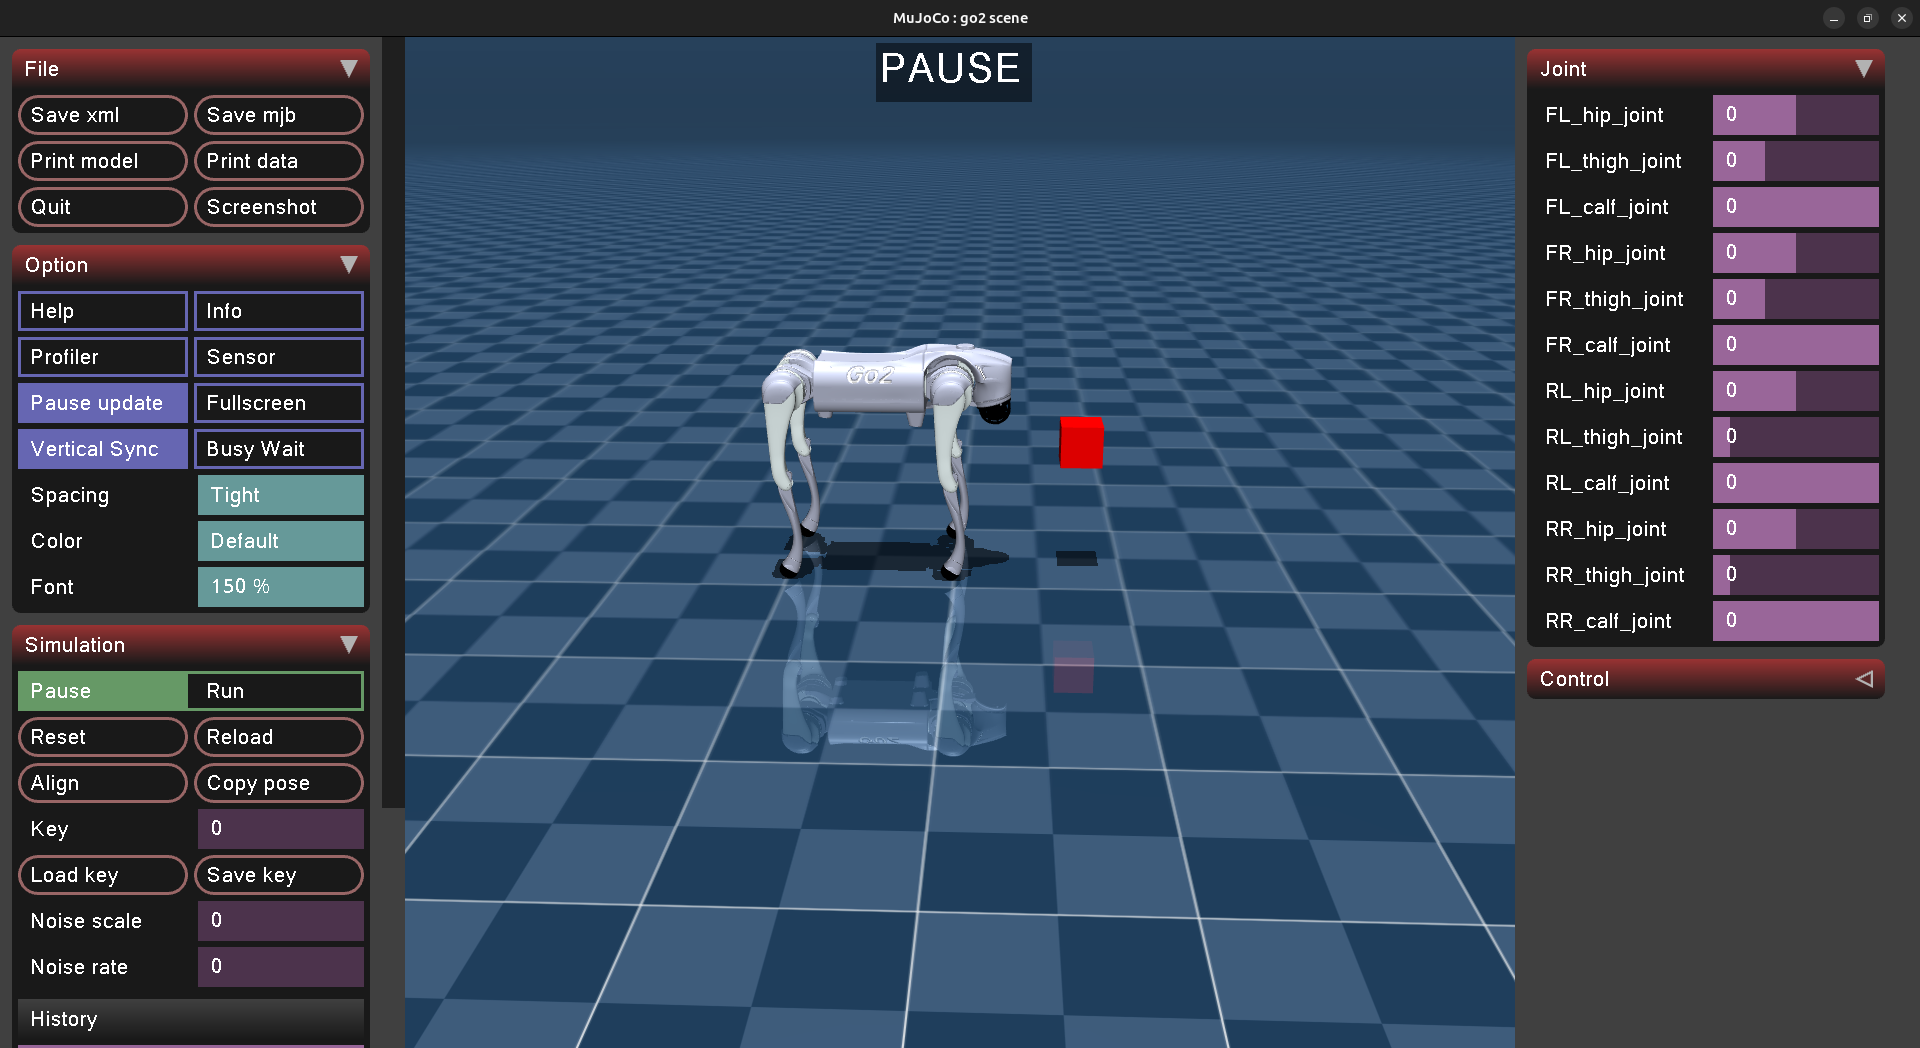
\includegraphics[width=0.75\textwidth]{imaxes/SimulacionGo2.png}
  \caption{Ventana de simulacion de MuJoCo.}
  \label{fig:Sim_Go2}
\end{figure}

Tras comprobar que esta simulación funcionaba correctamente se procedió con la creación del \gls{script}. A continuación, se muestra un pseudocódigo 
(figura \ref{lst:pseudocodigo_script_simulacion}) que refleja el funcionamiento general de este proceso.

\begin{lstlisting}[caption=Pseudocódigo del script de generación de datos para el modelo de mundo en simulación, label=lst:pseudocodigo_script_simulacion]
INICIO
  Cargar el modelo XML e inicializar las variables model y data
  Iniciar la simulación
  PARA cada episodio desde 1 hasta num_episodios HACER
    Reiniciar la posición del robot a la posición inicial
    Actualizar la simulación
    PARA cada iteración desde 1 hasta num_iteraciones HACER
      Obtener ObsT
      Seleccionar acción aleatoria
      Aplicar la acción seleccionada	
      Obtener ObsT+1
      Guardar los datos de la iteración
      Actualizar la simulación
    FIN PARA
  FIN PARA
  Guardar datos recopilados en un archivo para el posterior entrenamiento
FIN
\end{lstlisting}

Para comenzar, se definieron las variables de model y data como se ve anteriormente y se inicia la simulación de manera pasiva 
con \textit{“with mujoco.viewer.launch\_passive(model, data) as viewer:”} para que continúe mientras se ejecutan el resto de órdenes. 

Una vez iniciada, se procede a colocar el robot en posición erguida, preparado para comenzar a moverse. Los datos necesarios referentes a las posiciones de las articulaciones se 
obtienen del archivo \Gls{xml} “go2.xml” a través de \textit{“data.qpos[:] = model.key\_qpos”}. Después, se cargan estos datos en el robot para que se ejecuten con \textit{“mj.mj\_step(model, data)”} y se 
avanza la simulación con \textit{“viewer.sync()”}.

\begin{lstlisting}[language=Python]
  data.qpos[:] = model.key_qpos
  mj.mj_step(model, data)
  viewer.sync()
\end{lstlisting}

Una vez el robot se encuentra en la posición erguida, iniciamos el bucle principal, definido por la variable \textit{“num\_episodes”}. Dentro de este, anidamos otro bucle que avanzará 
las iteraciones de cada episodio. Al terminar cada uno de estos, se reinicia la configuración del robot a la posición por defecto para volver a comenzar a realizar movimientos. 

Los episodios terminarán bajo dos condiciones: que se alcance el número máximo de iteraciones especificado en el código o que el robot se caiga, es decir, que la simulación detecte 
que la altura del robot disminuye por debajo de un determinado valor. 

Esta última condición de parada se establece ya que, al considerar que el robot se caiga como una mala ejecución, se evita que se recopilen 
datos inútiles que entorpezcan el entrenamiento.

Durante una iteración se llevan a cabo los siguientes pasos:

 
\begin{itemize}
  \item Primero se guardan las observaciones del entorno en el instante actual (instante T), esto es, obtenemos los datos de posición y velocidad de las articulaciones del robot mediante 
        \textit{“data.qpos”} y \textit{“data.qvel”}, funciones que obtienen esta información del modelo del \Gls{xml}.

  \item Una vez guardado \( Obs_t \), seleccionamos una acción aleatoria mediante la función \textit{“get \_random\_action()”}. Esta recibe como parámetro el modelo del robot y devuelve un array de números aleatorios 
        comprendidos entre el límite inferior y superior de los actuadores. Destacar que esto se usó como primera aproximación para obtener acciones aleatorias y que, debido al problema que 
        comentaremos más adelante en esta sección, no se mejoró más el algoritmo en esta parte.

  \item Tras seleccionar la acción, ésta se aplica a los actuadores mediante \textit{“data.ctrl[:]”} y se hace avanzar la simulación con \textit{“mj.mj\_step(model, data)”}.

  \item Al realizar la acción, el robot se encuentra en el instante siguiente (es decir, en el instante T+1) por lo que repetimos el primer paso guardando las observaciones tras haber realizado 
        la acción.
  \item Después se procede a ordenar los datos de entrenamiento: se obtiene la posición del objetivo y se concatena tanto con las observaciones en T como en T+1, se concatena también las \( Obs_t \) con 
        la acción, formando así lo que llamaremos datos de entrada, y finalmente se añade a la lista de tuplas estos datos de entrada y los datos de salida (\( Obs_{t+1} \)) para el entrenamiento.
  \item Para terminar se actualiza la visualización de la simulación con \textit{“viewer.sync()”}.

\end{itemize}

\begin{lstlisting}[language=Python]
with mujoco.viewer.launch_passive(model, data) as viewer:


  # Colocar el robot en la posicion por defect
  data.qpos[:] = model.key_qpos
  mj.mj_step(model, data)
  viewer.sync()  


  for episode in range(num_episodes):
    
      n_iteration = 10000 # Numero maximo de iteraciones realizadas en cada episodio
      for iteration in range(n_iteration):
          obs_t = get_obs(data)  # Obtenemos las observaciones en T
          action = get_random_action(model)   #Obtenemos la accion aleatoria  
          data.ctrl[:] = action   # Aplica la accion
          mj.mj_step(model, data) # Avanza la simulacion
          obs_t1 = get_obs(data) # Obtenemos las observaciones en T+1


          # Guardar datos
          boxPos = np.copy(get_box_pos(data, box_id))
          datos_entrada = np.concat([np.concat([obs_t, boxPos]), action])
          trainnig_data.append((datos_entrada, np.concat([obs_t1, boxPos])))


          viewer.sync()   # Actualiza la visualizacion
        
          # Condicion de parada: si el robot se cae
          robot_height = data.qpos[2]  # Coordenada Z del cuerpo del robot
          if robot_height < 0.1:  # Si la altura es menor a un umbral, el robot esta caido
              print("Simulacion detenida por caida de robot en iteracion", iteration)
              break


      # Reiniciar la simulación al final de cada iteración
      data.qpos[:] = model.key_qpos
\end{lstlisting}


\subsection{Problemas durante la implementación}
\label{sec:desarrollo_problema_simulacion}

El principal problema de la implementación del entorno en simulación surgió durante el desarrollo del movimiento del robot, concretamente debido a la falta de las funciones 
de movimiento de alto nivel compatibles con este entorno.

Para conseguir que el robot realice acciones hay dos aproximaciones posibles: 

La primera es trabajando a alto nivel, utilizando el código y las funciones proporcionadas por el 
fabricante a través de su \Gls{sdk} en Github. Se trata de funciones cerradas, las cuales se desconoce los procesos internos que se realizan para devolver la solución.

La otra opción es trabajar a bajo nivel, indicando en el programa la fuerza que cada actuador debe realizar para obtener una acción específica.

Mientras que en el sistema real era posible emplear estas funciones de alto nivel para obtener el movimiento deseado, estas mismas funciones no estaban disponibles en el entorno de 
simulación. Esto implicaba que para conseguir desarrollar una locomoción útil, no bastaba con utilizar estas definiciones abstractas de las acciones, sino que era necesario aprender un 
controlador que transformara estas acciones a comandos a bajo nivel, capaces de producir una marcha funcional del robot. 

Este mismo riesgo ya se contempló en la planificación inicial, señalando que la falta de estas funciones o los problemas de implementación con MuJoCo podrían derivar en un retraso 
importante o incluso en eliminar esta parte del proyecto.

Para intentar solventar esta fase sin cancelar por completo el desarrollo en simulación, se intentó aprender un modelo simple de movimiento mediante aprendizaje automático con el fin de 
que realizara las acciones básicas requeridas, es decir, avanzar en línea recta una determinada distancia y girar sobre sí mismo en ambas direcciones. La intención de esta alternativa era disponer 
de un controlador sencillo que permitiera abstraer la complejidad del bajo nivel y continuar utilizando la simulación para entrenar los modelos de mundo y utilidad.

Sin embargo, los resultados obtenidos de este modelo no fueron satisfactorios. El movimiento del robot en estas pruebas era demasiado rudimentario, no conseguía desplazarse de manera 
correcta, por lo que se consideró que no proporcionaba una base adecuada para el aprendizaje de los modelos deliberativos y su posterior traslado al robot real.

Tras obtener estos resultados, se concluyó que, de continuar con el desarrollo de esta fase, implicaría consumir una parte excesiva del tiempo disponible para el proyecto en una tarea 
secundaria respecto al objetivo principal de este, poniendo en riesgo la finalización del trabajo. Aprender o diseñar un controlador para el Go2 en simulación requería un esfuerzo 
considerablemente mayor al previsto en un inicio. Además, centrarnos en este punto implicaría desviarse del objetivo de aprender modelos de mundo y de utilidad hacia la locomoción de bajo nivel. 

Por estos motivos, tras comentar la situación con los tutores, se llegó a la conclusión de cancelar esta parte y priorizar el desarrollo en el entorno real, donde sí existían funciones 
de alto nivel proporcionadas por el SDK del robot, siendo una solución más viable para completar el sistema deliberativo de manera satisfactoria. Esta decisión redujo el alcance del 
proyecto previsto inicialmente para la fase de simulación, sin embargo, permitió centrar los recursos  en las partes que se podían realizar dentro del plazo del proyecto, asegurando 
obtener resultados válidos en el entorno real.


\section{Desarrollo en robot cuadrúpedo}
\label{sec:desarrollo_robot_cuadrupedo}

Después de la cancelación de la fase de simulación, el desarrollo del proyecto pasó a centrarse en el entorno real con el robot cuadrupedo Unitree Go2. Esto permitió reorientar el trabajo hacia 
una alternativa más viable, gracias a disponer de funciones de control de alto nivel proporcionadas por el \Gls{sdk} del robot. Sumado a esto, se contaba con un sistema de captura de movimiento 
externo a través del sistema de cámaras Optitrack con el que se obtendrían las observaciones necesarias para el entrenamiento.

En esta fase se buscaba obtener los datos del entorno y del propio robot, almacenarlos de forma estructurada, entrenar modelos de mundo y de utilidad con dichos datos y, finalmente, validar el 
correcto funcionamiento de estos modelos con una demostración real.

Estos objetivos encajan con el alcance final asumido en el proyecto, que busca demostrar la viabilidad del aprendizaje de modelos en un entorno real, a pesar de no completar la parte 
de simulación.

En el siguiente enlace se puede acceder al repositorio de GitHub con el código del trabajo, así como el material audiovisual de las demostraciones del sistema:

\url{https://github.com/s-lopez5/TFG_GO2}

\subsection{Configuración del sistema Optitrack}
\label{sec:desarrollo_conf_optitrack}

El primer paso de esta configuración consistió en dejar completamente operativa la infraestructura de captura de movimiento. Como se explicó previamente en el apartado de Tecnologias 
Empleadas (sección \ref{sec:tecnologias_empleadas}, página \pageref{sec:tecnologias_empleadas}), dispondremos de un sistema Optitrack compuesto por 8 cámaras de Primex 13W distribuidas alrededor del espacio de trabajo, conectadas a un ordenador Intel NUC donde se 
ejecuta Motive. Este equipo fue el encargado de actuar a modo de servidor de streaming para transmitir los datos al ordenador del estudiante, en el que se ejecutaron los \gls{script}s de Python 
encargados del control del robot, la obtención de datos y del entrenamiento de los modelos. Para llevar a cabo esta puesta a punto del sistema se realizaron varias tareas de configuración 
que explicaremos a continuación.

En primer lugar, se procedió a la calibración del sistema de cámaras y del volumen de trabajo. Esta fase fue especialmente importante para asegurar que la posición obtenida del Motive fuese lo 
suficientemente precisa y estable para ser utilizada posteriormente para el entrenamiento de los modelos. El proceso a seguir para calibrar el sistema se encuentra explicado en el 
seccion \ref{sec:tecnologias_empleadas} (pagina \pageref{sec:tecnologias_empleadas}). 

Una vez completado este proceso, se verificó que el volumen de captura (ver figura \ref{fig:volumen_captura}, sección \ref{sec:entorno_optitrack}) se encontraba definido 
de manera correcta y que no se encontraban errores que pudiesen entorpecer la obtención de datos. Durante una de las calibraciones finales tras la instalación de las cuatro cámaras adicionales 
que llegaron a mediados del proyecto, se encontró que las cámaras nuevas presentaban unos puntos de ruido visual al captar la información. Al observar con detalle lo que registraba cada cámara, 
se comprobó que estas mostraban puntos (resaltados en rojo en la figura \ref{fig:captura_errores_camaras}) como si estuvieran detectando marcadores (o reflejos de ellos) en zonas donde en 
realidad no había nada.

\begin{figure}[hp!]
  \centering
  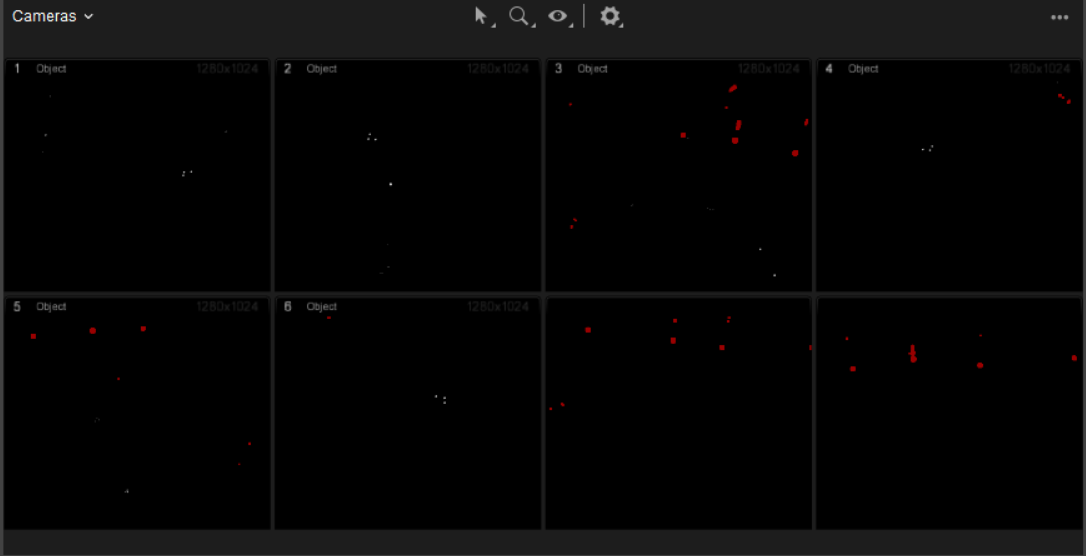
\includegraphics[width=\textwidth]{imaxes/CapturaErroresCamaras.png}
  \caption{Captura del ruido en las cámaras Optitrack (resaltados en rojo).}
  \label{fig:captura_errores_camaras}
\end{figure}

Tras varias pruebas para conseguir eliminar este ruido, ajustando la iluminación, limpiando 
las ópticas y cambiando la posición de las cámaras, se encontró que enmascarar estos puntos era la solución más viable en este momento. Esta función de Motive consiste en seleccionar los puntos 
que detectan las cámaras e indicar al sistema que los ignore, permitiendo obtener solo los datos reales correspondientes a los marcadores. Esta solución resultó especialmente importante ya que el 
sistema dependía completamente de la calidad de las observaciones obtenidas para el aprendizaje.

El siguiente paso consistió en preparar los objetos que necesitaban ser identificados en el entorno, es decir, el robot y el objetivo. Para ello, se colocaron marcadores reflectantes en ambos 
objetos. Para cada uno, se utilizaron tres marcadores distribuidos de manera triangular (en el caso del robot, se colocaron en la cabeza de este al ser la parte que más se acercará al 
objetivo). 

La decisión de utilizar tres marcadores en lugar de uno se tomó para permitir que, durante la captura de datos, pudiera calcularse el ángulo formado entre dos de ellos y emplearlo como referencia 
para que el modelo estimará la orientación del robot. Para determinar la posición de cada objeto, se utilizó como referencia el punto medio obtenido a partir de sus tres marcadores.

Esta configuración también permitió crear dos \gls{markerset}s independientes en Motive, uno para cada objeto, y asignarles los nombres “Go2” y “Objetivo”. Los \gls{markerset}s son agrupaciones 
definidas en Motive que contienen tres o más marcadores, a los cuales se les asigna un nombre para trabajar con ellos de forma conjunta.

Trabajar con los marcadores mediante \gls{markerset}s resultó indispensable: permitió que los scripts desarrollados pudieran separar automáticamente la información de cada objeto, además de ofrecer 
una visualización más clara y organizada dentro del programa.

Una vez calibradas las cámaras y definidos los \gls{markerset}s, fue necesario configurar el streaming de datos desde Motive hacia el ordenador Linux. En esta fase se habilitó el envío 
(streaming) de datos por red y se seleccionó el modo Unicast. Se eligió este modo, y no el Multicast, porque al tratarse de una red con un único receptor no era necesario, además, al realizar 
pruebas con el modo Multicast no se consiguió establecer una conexión estable. 

También fue necesario establecer la configuración de red de manera que se pudiera entablar la conexión entre equipos sin errores. Para esto fue necesario verificar que la IP del servidor, el 
envío por UDP, los puertos de comunicación y la propia configuración de red tanto del Intel NUC como del ordenador Linux estuvieran configurados correctamente. Aunque en teoría esta parte parecía 
relativamente fácil de implementar, en la práctica se presentaron varios problemas en la configuración de la conexión que retrasaron brevemente la puesta en marcha del sistema. Destacar el 
ya mencionado problema con el modo Multicast, que se soluciono utilizando el modo Unicast, además de problemas con la configuración de las IPs y los puertos en los distintos equipos. El 
problema más destacable referente a la conexión surgió cuando se intentó conectar simultáneamente al ordenador principal el robot Go2 mediante cable ethernet y el NUC mediante WiFi. El 
equipo detectaba que dos dispositivos intentaban conectarse a la interfaz de red y le daba prioridad a uno de ellos (en este caso el robot Go2 al conectarse vía ethernet) dejando 
al otro sin conexión. Para solventarlo fue necesario crear interfaces de red distintas para cada una de las redes, así como asignarles IPs a cada una de ellas, a través de la terminal de Ubuntu.

Con el streaming de datos funcionando de manera correcta, se integró el \Gls{sdk} de NatNet en Python. Este se encargaba de recibir los paquetes \Gls{udp} enviados por Motive y traducir la información 
a los datos referentes a la posición de los objetos captados. Para esto fue necesario adaptar la recepción para filtrar los datos relevantes a través de los nombres de los \gls{markerset}s y separar la 
información adicional que transmite el programa. Esta modificación permitió obtener la posición de cada uno de los marcadores asignados a los \gls{markerset} para procesarla posteriormente en 
el \gls{script}.

El código de NatNet proporcionado en el repositorio se utilizó en su mayoría sin modificaciones. Los cambios se realizaron en el fichero “NatNetClient.py”, en el que se define la 
clase que le da nombre, “NatNetClient”, así como los atributos y métodos necesarios para su funcionamiento. Los cambios realizados fueron los siguientes: 

\begin{itemize}
  
  \item Por un lado, se añadieron a la clase los atributos de \textit{last\_pos}, un array en el que se guardará la última posición obtenida del robot para poder enviarla al \gls{script} principal 
  cuando sea necesaria, y \textit{obj\_pos}, array en el que se guarda la última posición del objetivo.
  \item Por otro lado, se añadieron los métodos getter para poder acceder a la informacion de estos atributos desde fuera de la clase.

\end{itemize}

\begin{lstlisting}[language=Python]
  #Getter para obtener la ultima posicion recibida
   def get_last_pos(self):
       return self.last_pos


   #Getter para obtener la posicion objetivo
   def get_objetive_pos(self):
       return self.obj_pos
\end{lstlisting}

Por último, en el método “\textit{\_\_process\_message}”, encargado de tratar los mensajes enviados con Motive, se añadió la función de filtrar la información enviada a través del nombre de los 
\gls{markerset}. De esta manera se permitía acceder a la posición de cada uno de los objetos por separado, con el fin de tratar cada una de manera independiente. En el caso del robot, la 
posición se guardó sin cambios para ser modificada en el \gls{script} principal. En cuanto a la posición del objetivo, se simplificó calculando el punto medio de los tres marcadores en lugar de 
guardar toda la información, ya que únicamente necesitamos un punto con el que trabajar.

\begin{lstlisting}[language=Python]
  if message_id == self.NAT_FRAMEOFDATA:
           trace("Message ID : %3.1d NAT_FRAMEOFDATA" % message_id)
           trace("Packet Size: ", packet_size)


           offset_tmp, mocap_data = self.__unpack_mocap_data(data[offset:], packet_size, major, minor) #type: ignore  # noqa E501
           offset += offset_tmp
          
           if print_level >= 1:
               self.last_pos = []


               #Obtener datos de los markers
               if mocap_data.marker_set_data:
                   for i, marker_data in enumerate(mocap_data.marker_set_data.marker_data_list):
                       if marker_data.model_name.decode('utf-8') == "Objetivo2":


                           x1, y1, z1 = marker_data.marker_pos_list[0]
                           x2, y2, z2 = marker_data.marker_pos_list[1]
                           x3, y3, z3 = marker_data.marker_pos_list[2]


                           self.obj_pos = [(x1 + x2 + x3) / 3, y1, (z1 + z2 + z3) / 3]




                       elif marker_data.model_name.decode('utf-8') == "Go2":
                           self.last_pos = marker_data.marker_pos_list
\end{lstlisting}

\subsection{Configuración del robot Unitree Go2}
\label{sec:desarrollo_conf_go2}

En paralelo a la configuración del sistema de Optitrack fue necesario preparar el robot Unitree Go2 para su funcionamiento e integración con los demás componentes del sistema. La primera 
tarea consistió en establecer la conexión entre el robot y el ordenador desde el que se ejecutaron los \gls{script}s de control. Para ello se utilizó una conexión Ethernet, ya que en el momento 
el \Gls{sdk} no soportaba vía WiFi y esta era la única manera de enviar instrucciones desde el código. Fue necesario utilizar un cable con la suficiente longitud (en nuestro caso se utilizó un 
cable de 15 metros) para permitir al robot moverse libremente dentro del volumen de captura sin comprometer su integridad.

Una vez establecida la conectividad, se realizaron pruebas básicas con el \Gls{sdk} en Python para comprobar que el ordenador era capaz de comunicarse de manera correcta con el robot y este 
recibiera los comandos. Estas comprobaciones buscaban asegurar que el sistema podía enviar órdenes y el robot era capaz de recibirlas y realizarlas. A partir de aquí se procedió a comprobar 
las distintas posibilidades de control que ofrece el \Gls{sdk} para seleccionar cuales se utilizarían. 

Aunque el \Gls{sdk} permite trabajar también a bajo nivel, ya se indicó en puntos anteriores que se optó por utilizar únicamente las funciones de control de movimiento de alto nivel del 
robot, con el fin de evitar la complejidad asociada a trabajar directamente con los actuadores, evitando de esta manera encontrarse con problemas como ocurrió con el entorno simulado. Esta 
decisión permitió mantener el foco en el aprendizaje de modelos deliberativos, siendo además coherente con el análisis de riesgos para evitar que el desarrollo quedase bloqueado por problemas 
con la locomoción.

Entre las funciones de control proporcionadas por Unitree, se utilizaron las necesarias para generar el movimiento básico del robot. Concretamente, se utilizó la función 
\textit{sport\_client.Move()} para transmitirle al robot el tipo de movimiento que debe realizar, así como \textit{sport\_client.StopMove()} para indicarle que se detenga. Para que el robot 
adoptase la posición de pie o se tumbase, se emplearon las funciones \textit{sport\_client.StandUp()} y \textit{sport\_client.StandDown()} respectivamente. Por último, la 
función \textit{sport\_client.ClassicWalk()} permitía configurar el robot en el modo de movimiento por defecto.

Con este enfoque, se definió un conjunto de acciones simples y discretas que el robot pudiera ejecutar de manera fiable y que permitieran moverse por el espacio de trabajo de manera 
controlada. El sistema no necesitaba explotar al máximo la complejidad motriz del robot, únicamente se necesitaba un conjunto de movimientos reducidos que permitiera generar experiencias 
significativas para el entrenamiento. Por lo tanto, las acciones que se plantearon fueron desplazamientos en línea recta y giros sobre sí mismo, ambos con distintas opciones de distancia 
y ángulo para que el sistema entrenado eligiera cual le convenía más. Se probaron varias configuraciones de estas acciones para ver cuál se adaptaba mejor al entorno, pero finalmente se 
optó por utilizar tres opciones de velocidad de desplazamiento (0.3m/s, 0.5m/s y 0.7m/s) y tres opciones de velocidad de giro para cada uno de los sentidos (0.524 rad/s, 0.785 rad/s y 
1.047 rad/s). Esta simplificación permitió relacionar de forma clara cada acción con el cambio en la posición del robot respecto al objetivo, siendo esto especialmente relevante para 
la creación del conjunto de datos para entrenar los modelos de mundo y de utilidad.

Estas acciones se realizaban a través del cliente del \Gls{sdk}, \textit{sport\_client}, utilizando la función \textit{sport\_client.Move(accion[0], accion[1], accion[2])}. El primer parámetro es 
el que indica la velocidad en línea recta que debe avanzar el robot, en la que se utilizan los valores antes mencionados. El segundo parámetro corresponde con la velocidad de desplazamiento 
lateral, que en este caso no se utilizará y tendrá siempre el valor 0. En cuanto al último parámetro, hace referencia a la velocidad de giro sobre el eje vertical en rad/s, tambien con los 
valores mencionados anteriormente.

Antes de comenzar con la obtención de datos, fue necesario realizar unas serie de pruebas de seguridad. En ellas se especificaron los límites del área de trabajo en la cual el robot iba a 
operar (figura \ref{fig:entorno_trabajo}). Estos límites se establecieron desde un punto de vista conservativo para garantizar la seguridad del robot, dado que el otro robot Go2 con el que contaba el centro estaba en reparaciones 
por haberse dañado. También se definieron teniendo en cuenta el espacio que captaban las cámaras sin perder el tracking del robot, además de la seguridad y el espacio que necesitaba este para 
maniobrar en caso de salirse de los límites. Estas precauciones responden a uno de los requisitos establecidos en la planificación, que exige mantener la seguridad del robot y del material 
durante las pruebas en entorno real.


\begin{figure}[hp!]
  \centering
  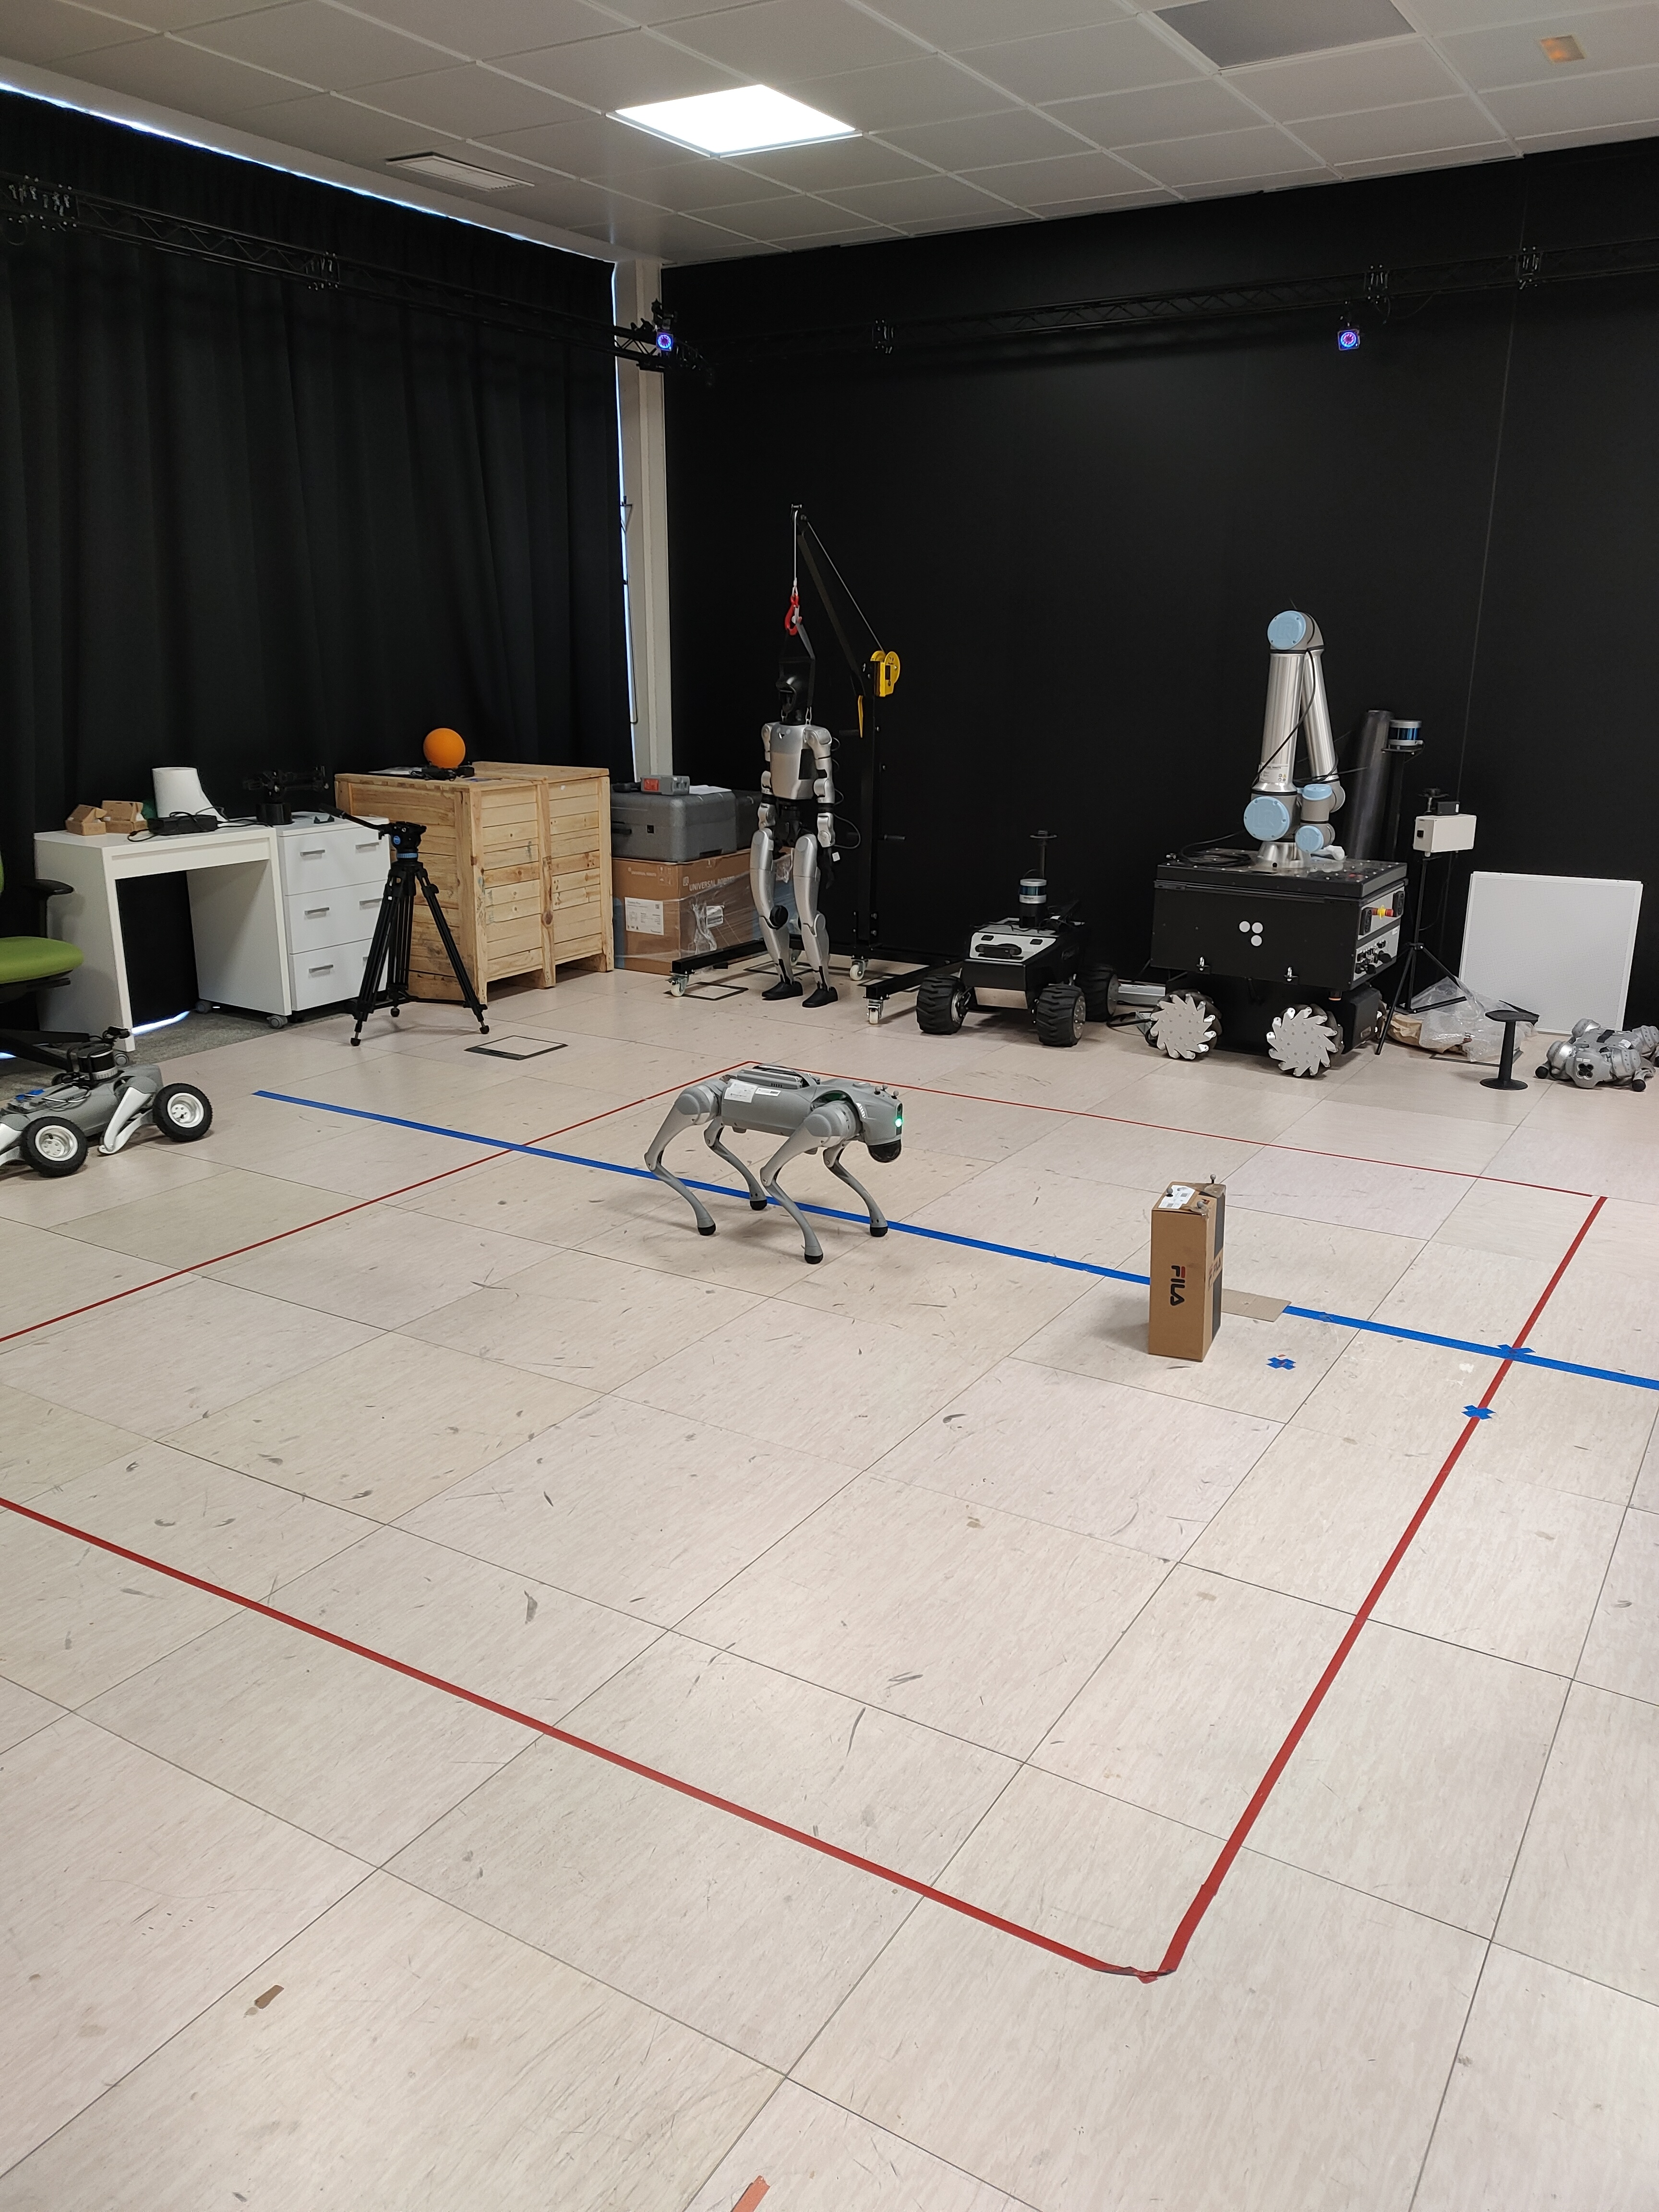
\includegraphics[width=0.5\textwidth]{imaxes/EntornoTrabajo.png}
  \caption{Limites del espacio de trabajo.}
  \label{fig:entorno_trabajo}
\end{figure}



\subsection{Modelo de mundo}
\label{sec:desarrollo_WM}

El primer resultado tangible del proyecto fue la obtención de un modelo de mundo funcional. El objetivo de este modelo, ya definido en los requisitos y en el desarrollo del sistema, era aprender 
la relación entre una observación actual del entorno, una acción realizada por el robot y la observación posterior a dicha acción.

\subsubsection{Obtención de datos para el modelo de mundo}

Una vez configurado tanto el sistema Optitrack como el robot, se procedió a desarrollar el \gls{script} que recopila los datos de entrenamiento para el modelo de mundo. Este programa será el 
encargado de producir un determinado número de episodios, en los cuales cada iteración genera la tupla de [\( Obs_t \), acción, \( Obs_{t+1} \)], donde cada observación incluye la información del 
estado del robot y del objetivo en un instante concreto, que se almacenará y se utilizará para el entrenamiento. Para lograr esto, el \gls{script} integra el \Gls{sdk} de NatNet para recibir las 
observaciones con el SDK encargado de controlar el robot y almacena de manera organizada los datos en listas utilizando la libreria Pickle para guardarlos en archivos .pkl que se utilizaran en el 
aprendizaje.

El funcionamiento general del \gls{script} consta de un bucle en el que se ejecutan las iteraciones y se guardan las tuplas de [\( Obs_t \), acción, \( Obs_{t+1} \)] en una lista para su posterior 
uso. 

Para comenzar, se inicializa el cliente de streaming para conectarse con Motive y el cliente del robot para enviarle órdenes a este, además se crean las variables necesarias y se configura el 
robot en el modo clásico de movimiento (modo de movimiento por defecto del robot).

Tras esto, lo primero es obtener las observaciones actuales del entorno a partir de la posición del robot y del objetivo captadas por Optitrack. Estas observaciones son una tupla formada por 
tres elementos:

\begin{itemize}
  \item La distancia entre el robot y el objetivo.
  \item El ángulo del robot con el objetivo respecto al origen (el punto [0,0,0]).
  \item El ángulo del propio robot respecto al origen (para esto se utiliza la posición de dos de los marcadores del robot).
\end{itemize} 

Para calcular la distancia utilizamos la fórmula 
\[
d = \sqrt{(x_{robot} - x_{objetivo})^2 + (y_{robot} - y_{objetivo})^2}
\]
y para calcular los ángulos se utiliza 
\[
\alpha = \arctan{(y_{robot} - y_{Z})^2 + (x_{robot} - x_{Z})^2}
\]
, siendo esta Z la posición del objetivo o del segundo marcador del robot en función del ángulo que se quiera calcular. 

Después de calcular las observaciones actuales, se selecciona aleatoriamente una de las acciones disponibles y se transmite esta orden al robot. En el caso del modelo de mundo, se elige, de 
entre las 9 opciones disponibles, una acción de manera aleatoria utilizando la librería Random. Tras esperar el tiempo necesario para que el robot complete la acción seleccionada, se comprueba 
que este no haya salido de los límites del entorno establecidos previamente. En caso de detectar que el robot se encuentra fuera de los límites, el programa ejecuta una rutina que devuelve el 
robot dentro de estos. Esta rutina se activa en el momento que, tras terminar de realizar una acción, las cámaras detectan que el robot se encuentra fuera de la zona preestablecida. Cuando esto 
sucede, el robot se detiene por completo, realiza un giro de 180º y avanza en línea recta hasta volver dentro de los límites. Tras esto, el robot retoma su rutina normal ejecutando acciones 
aleatorias. Esta iteración no queda registrada en los conjuntos de datos con el fin de evitar que entorpezca el futuro entrenamiento al considerar erróneo este comportamiento. En el caso 
contrario, el \gls{script} vuelve a consultar la posición del robot y calcula las nuevas observaciones.

Finalmente, se construye la tupla compuesta por el estado inicial, la acción seleccionada y el estado posterior y se añade a la lista de datos de entrenamiento. Este proceso se repite hasta 
construir un conjunto de datos suficiente.

Con el fin de lograr un modelo eficiente que fuese capaz de generalizar de manera adecuada, fue necesario obtener una cantidad suficiente de datos en los que se explore todo el espacio de 
trabajo. Además, para conseguir aumentar la cantidad de escenarios explorados, la posición del robot y del objetivo se modificaron en cada episodio.

Este proceso de recolección de datos llevó aproximadamente 2 semanas trabajando 4 horas diarias en los que finalmente se recolectaron un total de 1200 muestras que formaron el conjunto de 
datos con los que posteriormente se entrenaría el modelo de mundo.

Durante el desarrollo de este \gls{script} se prestó especial atención a la cohesión entre la ejecución de las acciones y la obtención de las observaciones. Siendo este uno de los puntos 
de riesgo identificados en la planificación, fue necesario introducir pausas manualmente para controlar que el estado posterior correspondiera a la acción ejecutada. Asimismo, también fue 
importante controlar las pérdidas de seguimiento, las cuales eran más frecuentes cuando solo había disponibles 4 cámaras en lugar de 8, y la salida de los límites del robot (proceso que 
se explicó previamente), evitando que datos incorrectos contaminaran el conjunto de entrenamiento.


\subsubsection{Entrenamiento del modelo de mundo}

Con los datos ya recopilados, la siguiente parte consistió en desarrollar el \gls{script} para entrenar el modelo de mundo. Este tiene como propósito aprender una función capaz de predecir la 
observación siguiente a partir de la observación actual y de la acción a ejecutar por el robot. Se implementó utilizando la librería Keras de TensorFlow.

El primer paso fue cargar el conjunto de datos generado previamente. Para esto, se utiliza nuevamente la librería Pickle, con la que se guardaron los datos en el \gls{script} anterior. Después 
se realiza el preprocesado necesario: Se separan los datos en entradas y salidas, se normalizan los valores de los datos y se dividen en dos subconjuntos de entrenamiento y de validación, en 
este caso utilizando un reparto de 80\%-20\% respectivamente.

El proceso de normalización mencionado consiste en transformar los valores de las entradas y salidas en una escala común con el objetivo de mejorar el entrenamiento. En este caso, se realizó 
mediante una estandarización basada en la media y la desviación típica de cada variable. Para esto, se calculó la media y la desviación típica de cada uno de los componentes de los conjuntos 
de entradas y salidas utilizando las fórmulas:

La media:

\[
\mu = \frac{1}{n}\sum_{i=1}^{n} x_i
\]

y la desviación típica:

\[
\sigma = \sqrt{\frac{1}{n}\sum_{i=1}^{n}(x_i - \mu)^2}
\]

donde \(n\) representa el número total de muestras y \(x_i\) cada uno de los valores de la variable.

Para cada variable, se restó a cada valor la media de dicha variable y el resultado se dividió entre la desviación típica, como se puede apreciar en la siguiente fórmula:

\[
x_{\text{norm}} = \frac{x - \mu}{\sigma}
\]

Donde \(\mu\) es la media de esa variable, y \(\sigma\) es su desviación típica.

De esta manera se consigue que los datos obtengan una media próxima a 0 y una desviación típica cercana a 1.

A continuación, se definió la arquitectura de la red y los hiperparametros con los que se entrenaría el modelo. Se utilizó una red de neuronas formada por 4 capas, con una densidad de 128, 
256, 128 y 64 respectivamente. Para la compilación del modelo se utilizó el optimizador Adam proporcionado por Keras y se usó como métricas el error cuadrático medio (MSE) y el error medio 
absoluto (MAE). A mayores, se establecieron dos callbacks para el entrenamiento: por un lado, se creó un EarlyStop para detener el entrenamiento en caso de no mostrar mejora durante 50 épocas, 
por otro, se añadió una reducción del learning rate cada 20 épocas para evitar el sobreajuste del modelo.

Tras entrenar el modelo, proceso que llevó aproximadamente 5 minutos, se crearon dos gráficas que permiten evaluar su rendimiento:

En la figura \ref{fig:WM_training_hist} se muestra la evolución del entrenamiento del modelo de mundo en dos partes: la parte de la izquierda muestra el error cuadrático medio (MSE), representado 
como pérdida o loss, mientras que la parte de la derecha muestra la evolución del error absoluto medio (MAE). En ambas gráficas se puede apreciar cómo disminuye de manera progresiva el 
error a medida que avanzan las épocas, especialmente durante las primeras iteraciones. Además, las curvas tanto del conjunto de entrenamiento como del de validación presentan una evolución 
similar. Esto indica que el modelo es capaz de generalizar de manera adecuada sobre nuevos datos.

\begin{figure}[hp!]
  \centering
  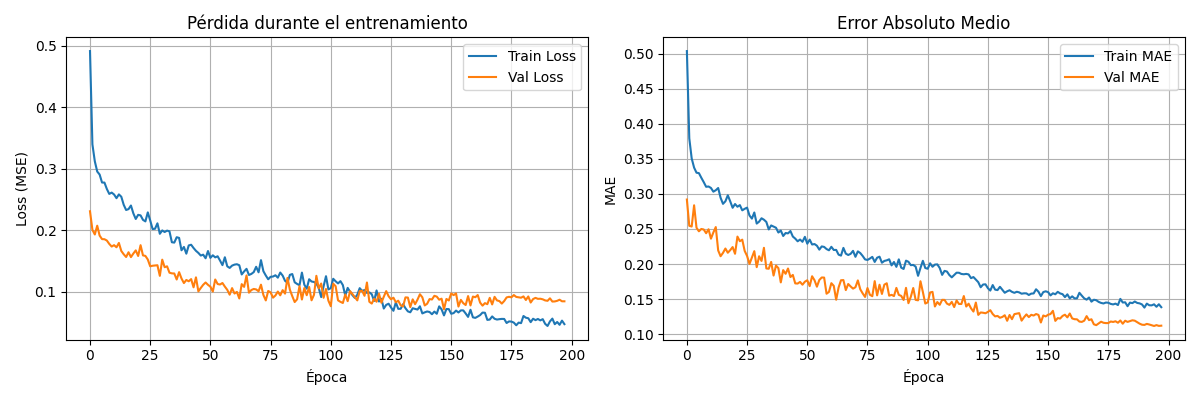
\includegraphics[width=\textwidth]{imaxes/WM/WM_training_hist.png}
  \caption{Historial de entrenamiento del modelo de mundo.}
  \label{fig:WM_training_hist}
\end{figure}

Por otro lado, la figura \ref{fig:WM_predicciones} compara las predicciones realizadas por el modelo con los valores reales de un conjunto de 50 ejemplos. Esta figura se divide en 3 
subgraficas, una para cada uno de los valores que se utilizan como observaciones (distancia, ángulo con el objetivo y ángulo sobre sí mismo). En los tres casos se puede observar como la 
mayoría de las predicciones son acertadas o se presentan muy poco error, lo que indica que el modelo es capaz de aproximar de manera correcta el estado siguiente a una observación tras 
ejecutar una acción.

\begin{figure}[hp!]
  \centering
  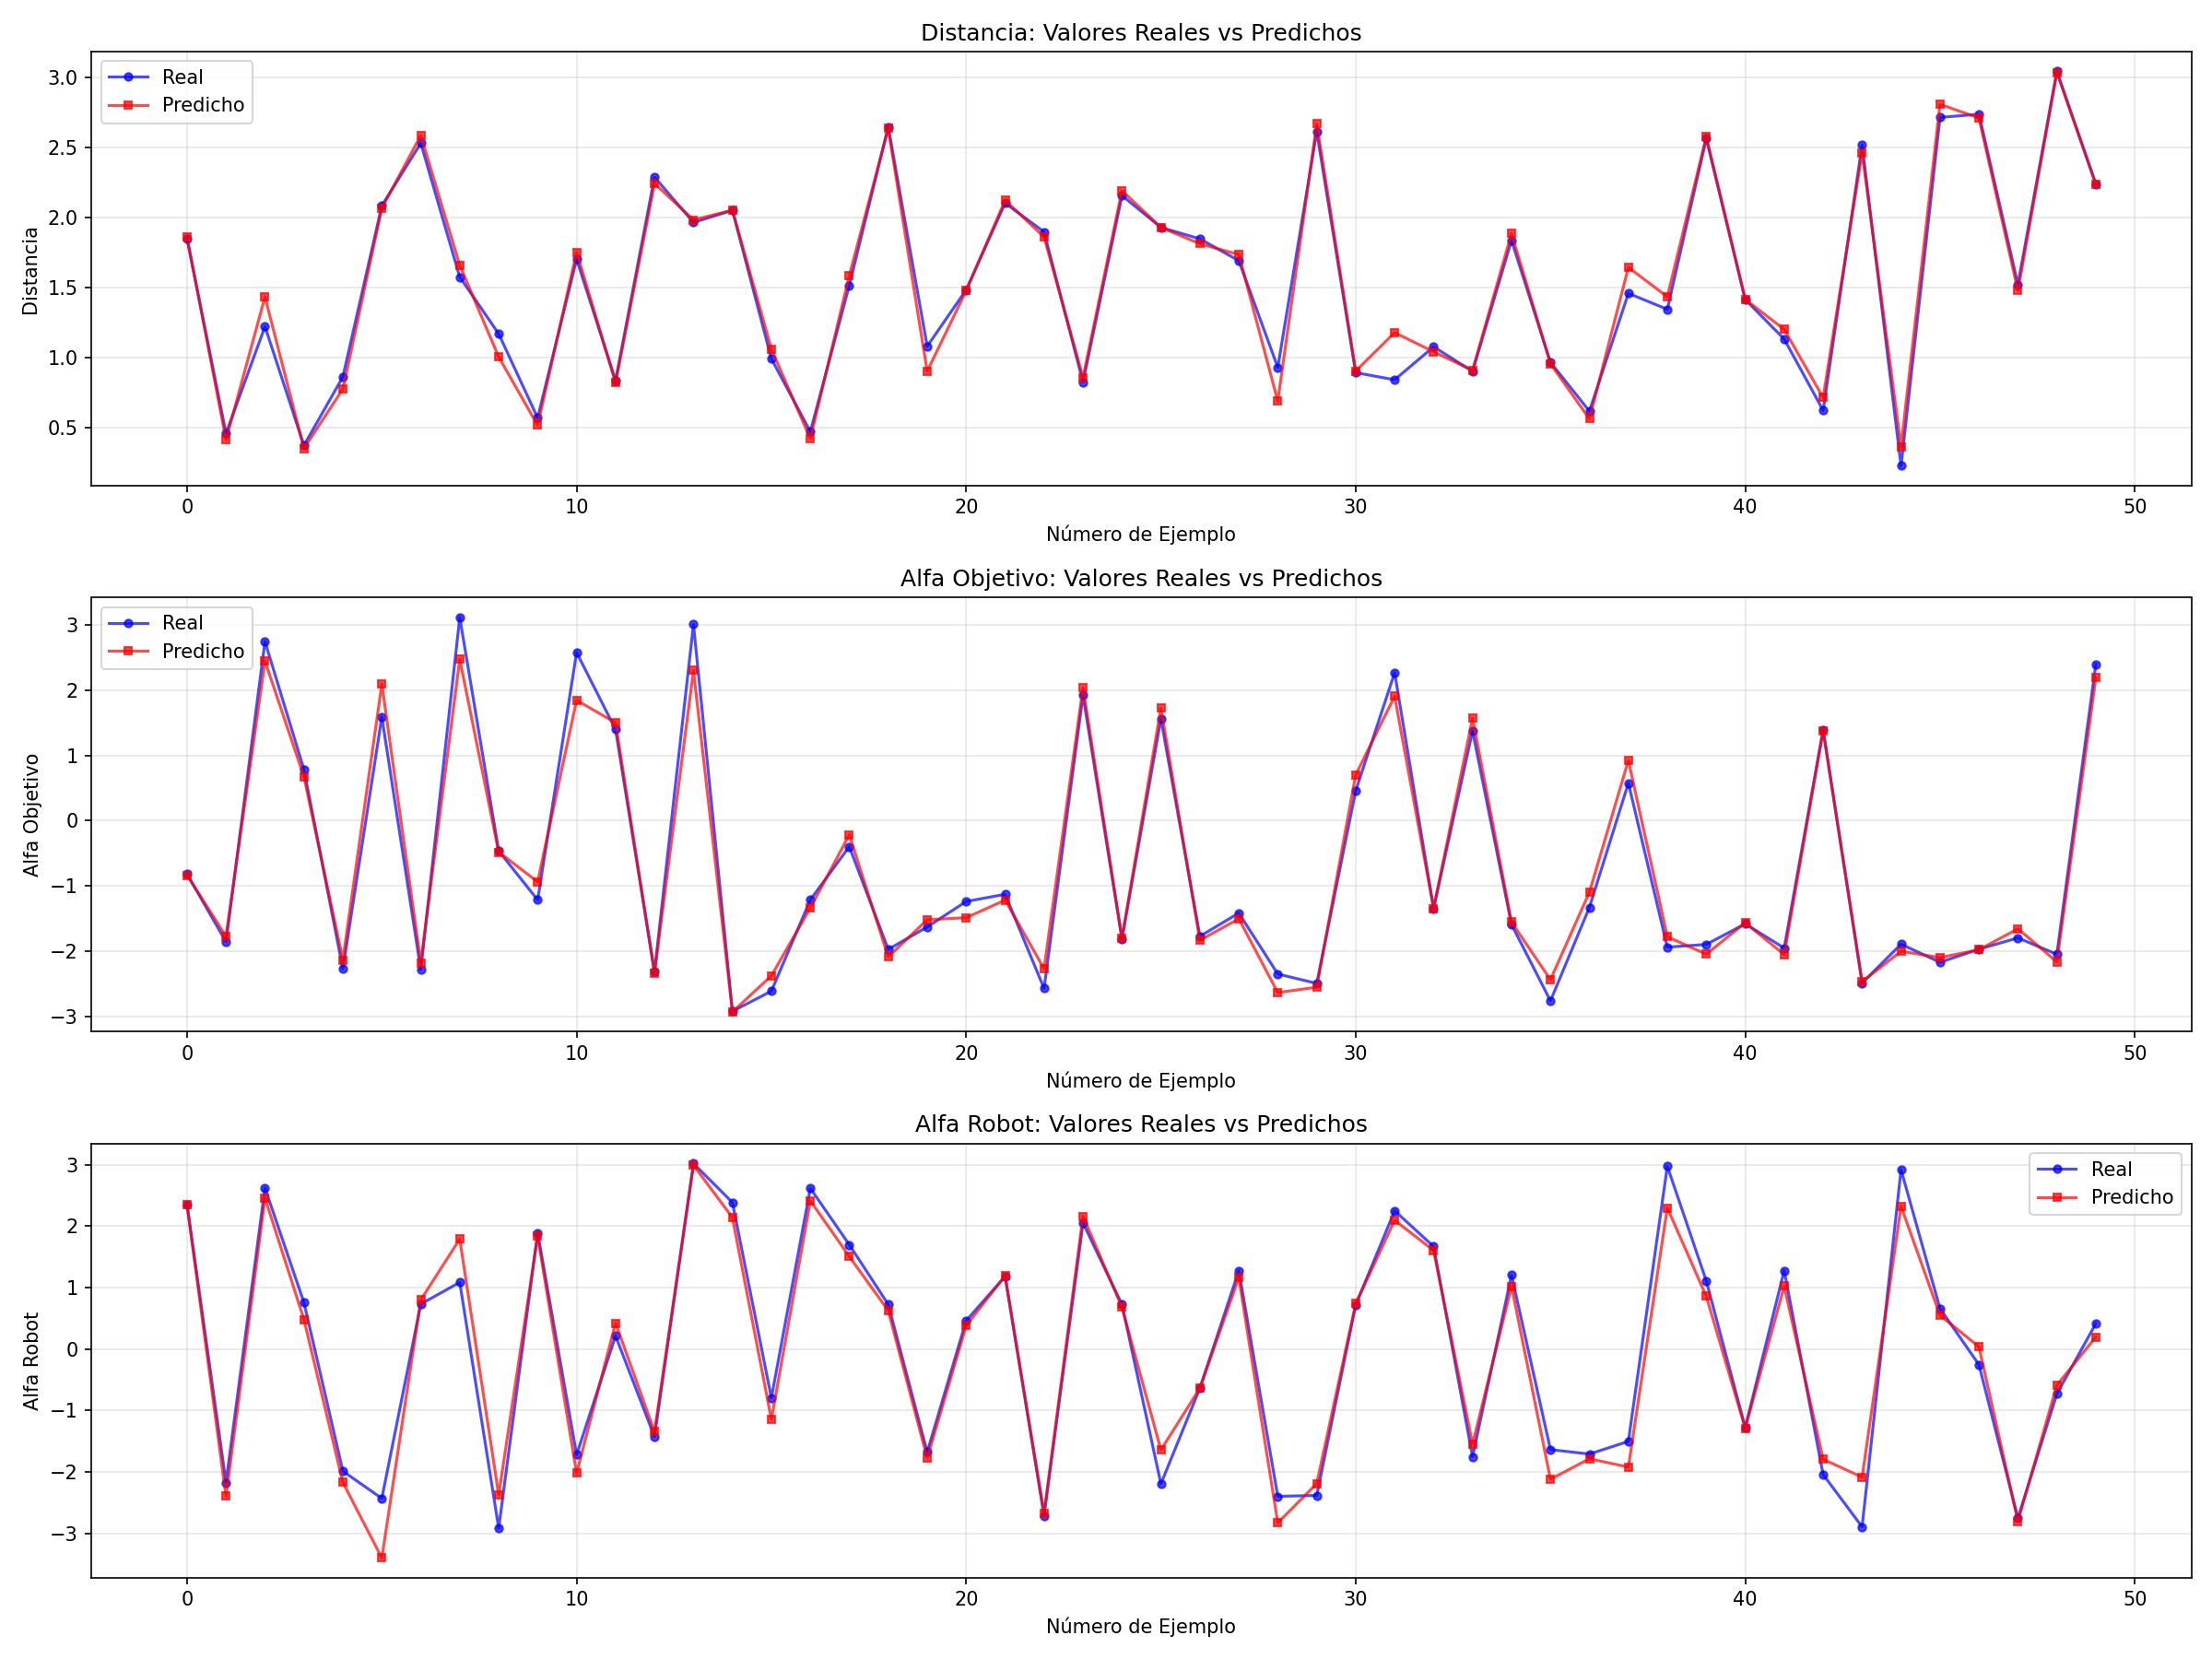
\includegraphics[width=\textwidth]{imaxes/WM/WM_predicciones.png}
  \caption{Predicciones del modelo de mundo.}
  \label{fig:WM_predicciones}
\end{figure}

En conjunto, los resultados presentados en ambas figuras permiten determinar que el modelo de mundo entrenado consigue aprender satisfactoriamente la dinámica del entorno en el dominio 
concreto del proyecto. Esto quiere decir, que a partir de la observación actual y la acción a realizar, el sistema es capaz de predecir con suficiente precisión la observación posterior, 
cumpliendo de esta manera el objetivo de este modelo dentro del sistema deliberativo.

\subsection{Modelo de utilidad}
\label{sec:desarrollo_UM}

El segundo resultado del proyecto fue la creación de un modelo de utilidad capaz de asignar un valor de utilidad a los estados percibidos por el robot en función del objetivo 
establecido. Mientras que el modelo de mundo era el encargado de responder a la pregunta de qué ocurriría si se lleva a cabo cierta acción, el modelo de utilidad responde a que tan útil 
será el estado resultante para alcanzar la meta perseguida. En el caso concreto de este trabajo, esta meta consiste en que el robot sea capaz de acercarse a un objetivo.

\subsubsection{Obtención de datos para el modelo de utilidad}

Una vez entrenado el modelo de mundo, el siguiente paso es la creación del \gls{script} encargado de recopilar los datos para el entrenamiento del modelo de utilidad. A diferencia del caso 
anterior, en el modelo de utilidad no se busca modelar la transición de un estado a otro, sino asociar a cada observación un valor que refleje su grado de utilidad en función del objetivo del 
sistema. En el caso de este proyecto, se busca que el robot sea capaz de acercarse a un objeto. Esta distancia se medirá en un rango de 0 a 1, por lo que, cuanto más cerca se encuentre el 
robot de este objeto, más cercano a 1 será el valor de utilidad asociado a esa observación.

Para generar los datos necesarios para el entrenamiento, el robot se desplaza por el entorno realizando acciones aleatorias hasta conseguir acercarse lo suficiente al objetivo. A medida que 
se generen los primeros modelos de utilidad, estas acciones se elegirán empleando estos primeros modelos sencillos en lugar de la aleatoriedad.

El objetivo de este \gls{script} era generar una lista de pares [\( Obs_{t+1} \), utilidad]. Mediante esta estructura, el sistema asignaba un valor de utilidad a cada una de las observaciones del 
camino que llevaron al robot hacia el objetivo en cada episodio. Para esto, se utilizó un método parecido al utilizado para generar los datos para el modelo de mundo: El sistema genera 
iteraciones realizando acciones de manera aleatoria para explorar el máximo espacio de acciones posibles.

A diferencia del \gls{script} anterior, en este caso cada iteración únicamente almacena una lista con las observaciones del instante siguiente (\( Obs_{t+1} \)). Además, se incorpora un 
criterio de parada: el episodio finaliza con éxito cuando el robot alcanza el objetivo. Cuando esto ocurre, el robot debe detenerse, para ello se indica al robot que pare y que se tumbe, 
dando por finalizada la ejecución. Tras esto, se recolocará tanto el robot como el objetivo en una nueva posición para seguir recopilando nuevos datos.

Para cada episodio completado con éxito, se seleccionan los diez últimos valores de la lista de \( Obs_{t+1} \) y se les asigna un valor de 0 a 1 de forma descendente, de modo que la última 
observación (la correspondiente al momento en que el robot llega al objetivo) recibe la puntuación más alta. Con ello se pretende conservar las diez últimas posiciones del trayecto seguido 
por el robot y asociar a cada una un valor de utilidad, permitiendo que el sistema aprenda qué posiciones fueron determinantes para alcanzar el objetivo. De esta manera se genera el conjunto 
de datos con la estructura de [\( Obs_{t+1} \), utilidad] mencionada anteriormente.

Sin embargo, un único episodio con 10 muestras no era suficiente para entrenar un modelo que funcione correctamente. Para ello fue necesario generar varios conjuntos de datos, es decir, varios 
caminos seguidos por el robot hasta el objetivo, y juntarlos, creando de esta manera una especie de mapa de la utilidad asociada a cada estado. 

El proceso de recopilación de datos y entrenamiento del modelo de utilidad no se realizó en una sola etapa, como ocurrió con el modelo de mundo. En este caso, se dividió en varias etapas 
definidas por el número de muestras utilizado para su entrenamiento, a medida que esta cantidad de datos aumentaba se producían modelos mejores con los que continuar recopilando datos.

Para el primer modelo entrenado se ejecutaron 9 episodios con un total de 90 muestras que tardaron aproximadamente 9 horas en obtenerse. Durante estos primeros episodios las acciones se 
realizaron de manera aleatoria con el fin de obtener un primer modelo que comenzase a explorar posibles caminos hacia el objetivo. Este primer modelo de utilidad, al depender completamente de 
la exploración aleatoria para alcanzar el objetivo, fue el que más tiempo requirió invertir en la recopilación de datos. El tiempo necesario para obtener cada uno de los episodios varió 
ampliamente debido precisamente a la aleatoriedad de las acciones. En algunos casos, el robot encontraba el objetivo relativamente rápido utilizando poca cantidad de acciones, sin embargo 
algunos episodios requirieron hasta 300 acciones o más para alcanzarlo.

Una vez obtenida esta pequeña cantidad de muestras, se procedió a entrenar el primer modelo de utilidad (proceso que se explica en el apartado siguiente). Este primer modelo se utilizó como 
base para continuar recopilando datos de manera más precisa y eficiente que seleccionando acciones aleatorias. Para esto, se creó otro \gls{script} igual al explicado anteriormente con la 
diferencia en cómo se seleccionan las acciones a realizar. Se utilizó el modelo de mundo entrenado previamente y este modelo de utilidad inicial para elegir la acción más “útil” entre las 
disponibles.

El modelo de mundo predice, en función del estado en que se encuentra, cuál será el estado siguiente para cada una de las acciones. Con estos datos, el modelo de utilidad le asigna un valor 
de utilidad a cada uno de estos estados. La acción que produzca el estado con mayor valor será la elegida para ejecutarse. De esta manera, se actualiza el modelo de utilidad a medida que se 
generen nuevos datos y se entrenen modelos que funcionen mejor, con el fin de obtener datos cada vez más precisos.

Debido a que los primeros modelos de utilidad no eran fiables y no eran capaces de acercarse al objetivo de manera correcta el 100\% de las veces, se añadió un pequeño porcentaje de 
aleatoriedad (entre el 5\% y el 20\%) en la selección de las acciones para hacer que el sistema explorara nuevas rutas para cumplir su objetivo, evitando también el estancamiento en los 
modelos. Esto se implementó durante la fase de exploración para la toma de datos del modelo. Con los primeros modelos de utilidad más “pobres”, el porcentaje de aleatoriedad era mayor para 
ermitir que el sistema siguiera mejorando y explorando nuevas posibilidades para llegar hasta el objetivo. A medida que se creaban modelos más eficientes, se redujo este porcentaje al ya no ser 
tan necesario explorar nuevas rutas sino refinar el modelo existente.

En la etapa final de recolección de datos, se obtuvo un conjunto de datos de 100 episodios, que contaba con casi 800 muestras de [\( Obs_{t+1} \), utilidad]. A pesar de que para las últimas 
fases de este proceso, con modelos que comenzaban a aproximar relativamente bien, se requirió menos tiempo que para las iniciales, se tardó aproximadamente 2 semanas en obtener todos los datos 
necesarios para entrenar el modelo de utilidad final.

En esta etapa resultó especialmente importante la diversidad de los datos. Para que el modelo pudiera aprender la relación entre estado y utilidad fue necesario obtener observaciones 
correspondientes a diversas disposiciones espaciales tanto del robot como del objetivo. Esto incluye tanto situaciones favorables (por ejemplo, el objetivo se situaba en frente del robot) como 
complicadas (por ejemplo, el objetivo se encontraba a la espalda del robot), permitiendo al sistema adaptarse al espacio de trabajo completo.


\subsubsection{Entrenamiento del modelo de utilidad}

Con el conjunto de datos preparado, se desarrolló el \gls{script} de entrenamiento para el modelo de utilidad. El objetivo era aprender una función capaz de predecir el valor de utilidad 
asociado a una determinada observación del entorno en función del objetivo establecido.

Mientras que el modelo de mundo era el encargado de responder a la pregunta de qué ocurriría si se lleva a cabo cierta acción, el modelo de utilidad responde a que tan útil será el estado 
resultante para alcanzar la meta perseguida. En el caso concreto de este trabajo, esta meta consiste en que el robot sea capaz de acercarse a un objetivo.

Al igual que en el caso del modelo de mundo, el \gls{script} incluye la carga y el preprocesado de los datos, la definición de la red neuronal, la configuración de los hiperparametros y la 
posterior evaluación de los resultados de rendimiento del modelo. En este caso, la salida del modelo era un valor escalar continuo, por lo que el criterio de evaluación se centró en comprobar 
si el sistema era capaz de aproximar de manera estable la utilidad esperada para observaciones no vistas con anterioridad.

Como se comentó anteriormente, el proceso de entrenamiento del modelo de utilidad se realizó en varias etapas a medida que aumentaba el conjunto de datos utilizado. En cada una de estas etapas 
se utilizó una mayor cantidad de datos y se creó una red de neuronas más compleja con el fin de mejorar el rendimiento hasta alcanzar el modelo final.

El primer paso fue crear el modelo inicial de 9 episodios obtenidos realizando acciones aleatorias. Una vez se disponía de esta pequeña cantidad de muestras, se procedió a entrenar este primer 
modelo. Para ello, se siguió el mismo procedimiento empleado en el entrenamiento del modelo de mundo: se realizó el preprocesado de los datos, se normalizaron y se dividieron en los conjuntos 
de entrenamiento y validación.

Dado que el volumen de datos era reducido, se optó por una red neuronal de menor tamaño, compuesta por 2 capas con 16 y 8 neuronas, respectivamente. La configuración de los hiperparámetros se 
estableció de forma similar a la utilizada en el modelo de mundo: se empleó el optimizador Adam, se utilizaron como métricas el MSE y el MAE, y se incorporaron tanto un earlyStop como una 
reducción del learning rate.

Sin embargo, este no fue el modelo final utilizado para el sistema. Se requería uno más robusto que predijese de manera más precisa la utilidad de cada posición. Este primer modelo se utilizó 
como base para los siguientes entrenados con mayor cantidad de datos. A medida que aumentaba el conjunto de entrenamiento, también fue necesario modificar la red neuronal, aumentando su tamaño 
para que fuera capaz de generalizar de manera correcta el nuevo volumen de datos.

A lo largo de los sucesivos modelos se utilizaron dos arquitecturas de neuronas más. La primera, de tamaño intermedio, se comenzó a utilizar cuando el conjunto de datos superó los 35 episodios 
y estaba formada por 3 capas de 32, 64 y 32 neuronas. La siguiente, siendo la red más grande que se utilizó, constaba de 4 capas de 64, 128, 64 y 32 neuronas respectivamente y se utilizó para 
las versiones finales del modelo de utilidad.

El resultado final, como se comentó en el apartado anterior, fue un modelo entrenado con 100 episodios, los cuales tenían casi 800 muestras de [\( Obs_{t+1} \), utilidad].

\begin{table}[H]
    \centering
    \small
    \setlength{\tabcolsep}{4pt}
    \renewcommand{\arraystretch}{1.15}
    \rowcolors{2}{white}{udcgray!25}
    \begin{tabularx}{\textwidth}{
    >{\centering\arraybackslash}X|
    >{\centering\arraybackslash}X|
    >{\centering\arraybackslash}X}
    \rowcolor{udcpink!25}
    \textbf{Nº episodios} & \textbf{Nº muestras} & \textbf{Estructura de la red} \\
    9 & 90 & 16-8 \\
    21 & 174 & 16-8 \\
    35 & 282 & 32-64-32 \\
    50 & 413 & 32-64-32 \\
    80 & 628 & 32-64-32 \\
    100 & 788 & 64-128-64-32 \\
    \end{tabularx}
    \caption{Tabla resumen de los modelos de utilidad.}
    \label{tab:tabla_modelos_UM}
\end{table}

Con el fin de evaluar el rendimiento de los modelos, se crearon dos gráficas, al igual que en el modelo de mundo, con las que se puede apreciar los resultados de estos:

En la figura \ref{fig:UM_training_hist} se muestra la evolución del entrenamiento mediante dos métricas: el MSE y el MAE. En ambas gráficas se observa una reducción del error durante las 
primeras épocas, seguida de una estabilización de las curvas. Esto indica que el modelo fue capaz de aprender la relación entre las observaciones del entorno y el valor de utilidad asignado, 
además de generalizar de manera adecuada sobre datos nuevos.

\begin{figure}[hp!]
  \centering
  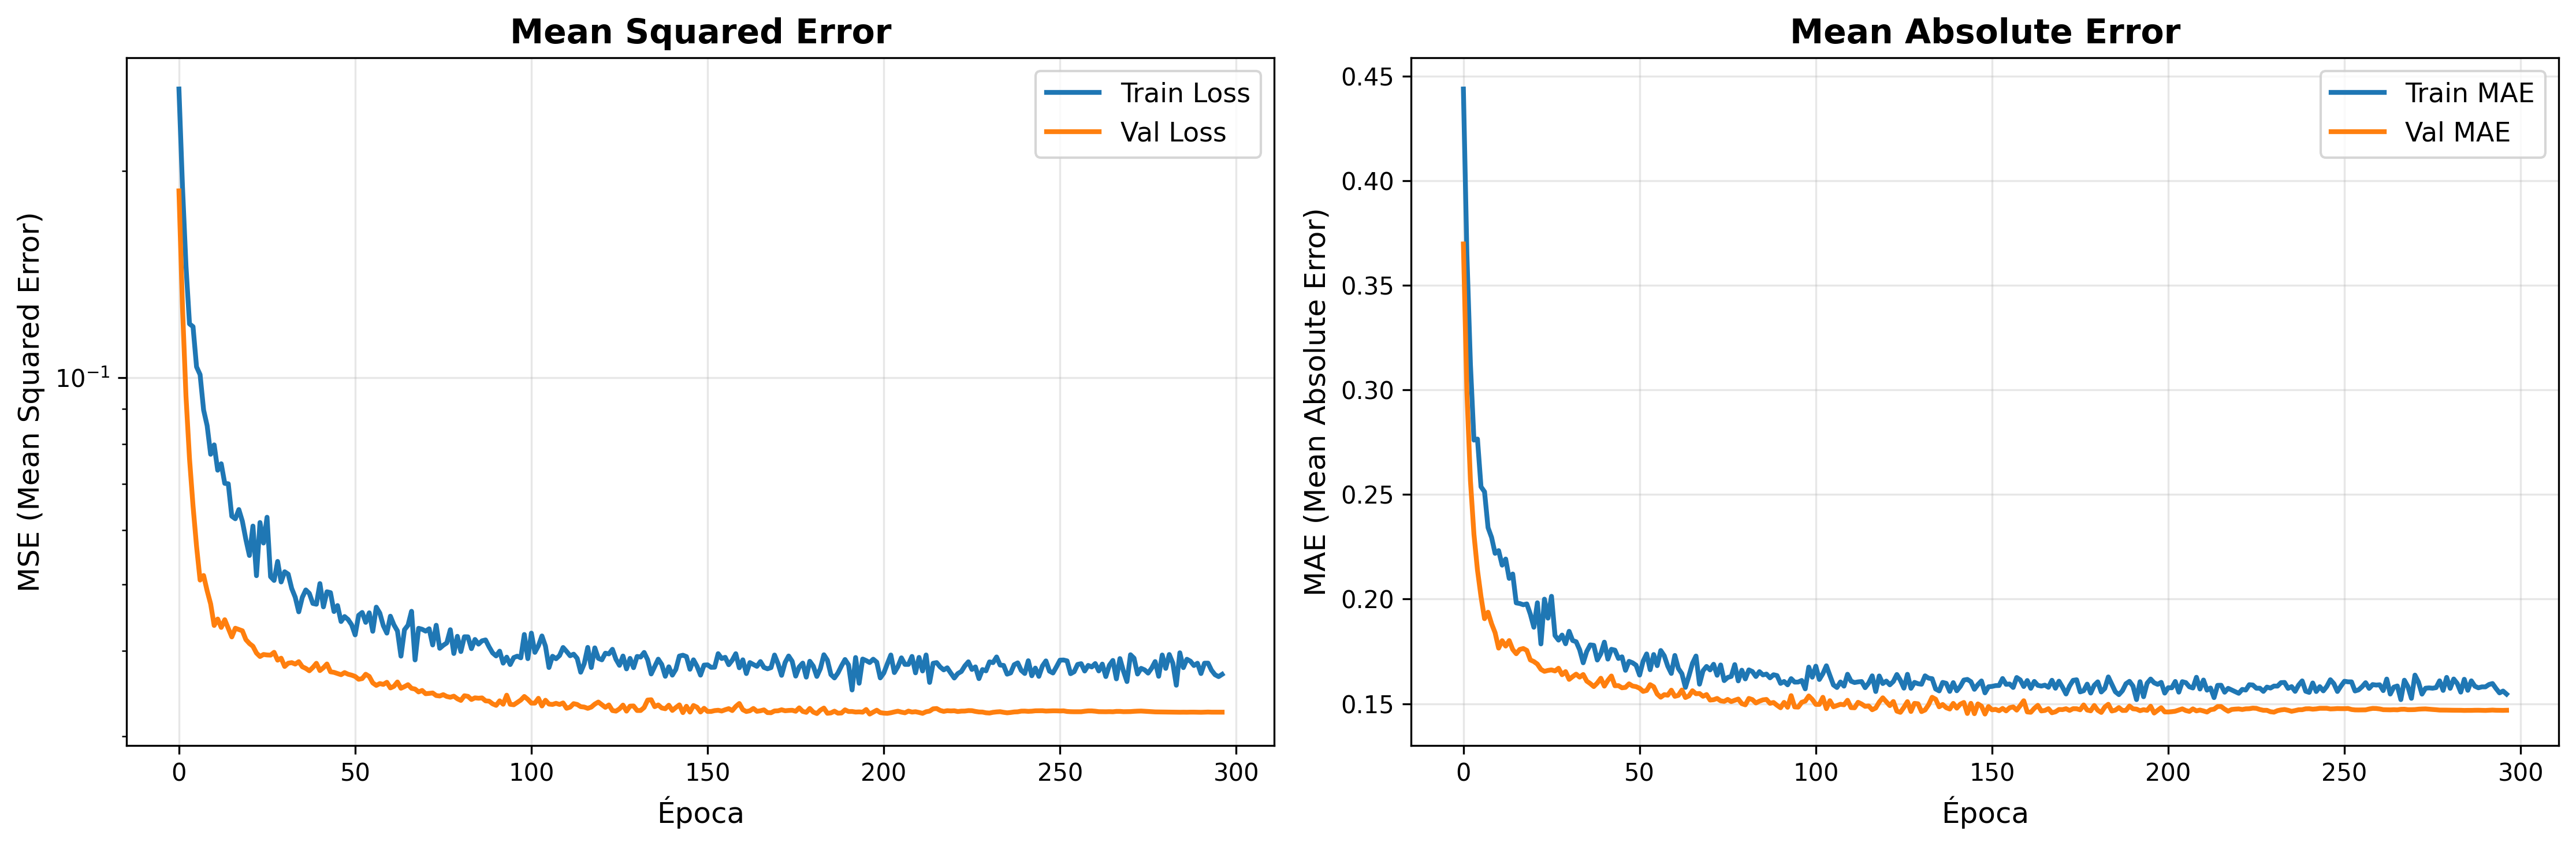
\includegraphics[width=\textwidth]{imaxes/UM/UM_training_hist_100.png}
  \caption{Historial de entrenamiento del modelo de utilidad.}
  \label{fig:UM_training_hist}
\end{figure}

En cuanto a la figura \ref{fig:UM_predicciones_100}, en esta se muestra la comparación entre los valores de utilidad reales y las predicciones realizadas por el modelo para un conjunto de 
ejemplos. En esta gráfica se observa que en general las predicciones siguen la misma tendencia que los valores reales. Esto quiere decir que el modelo es capaz de diferenciar entre estados 
más útiles, asociados a posiciones más cercanas, y estados menos útiles, correspondientes a estados más lejanos y menos útiles.

\begin{figure}[hp!]
  \centering
  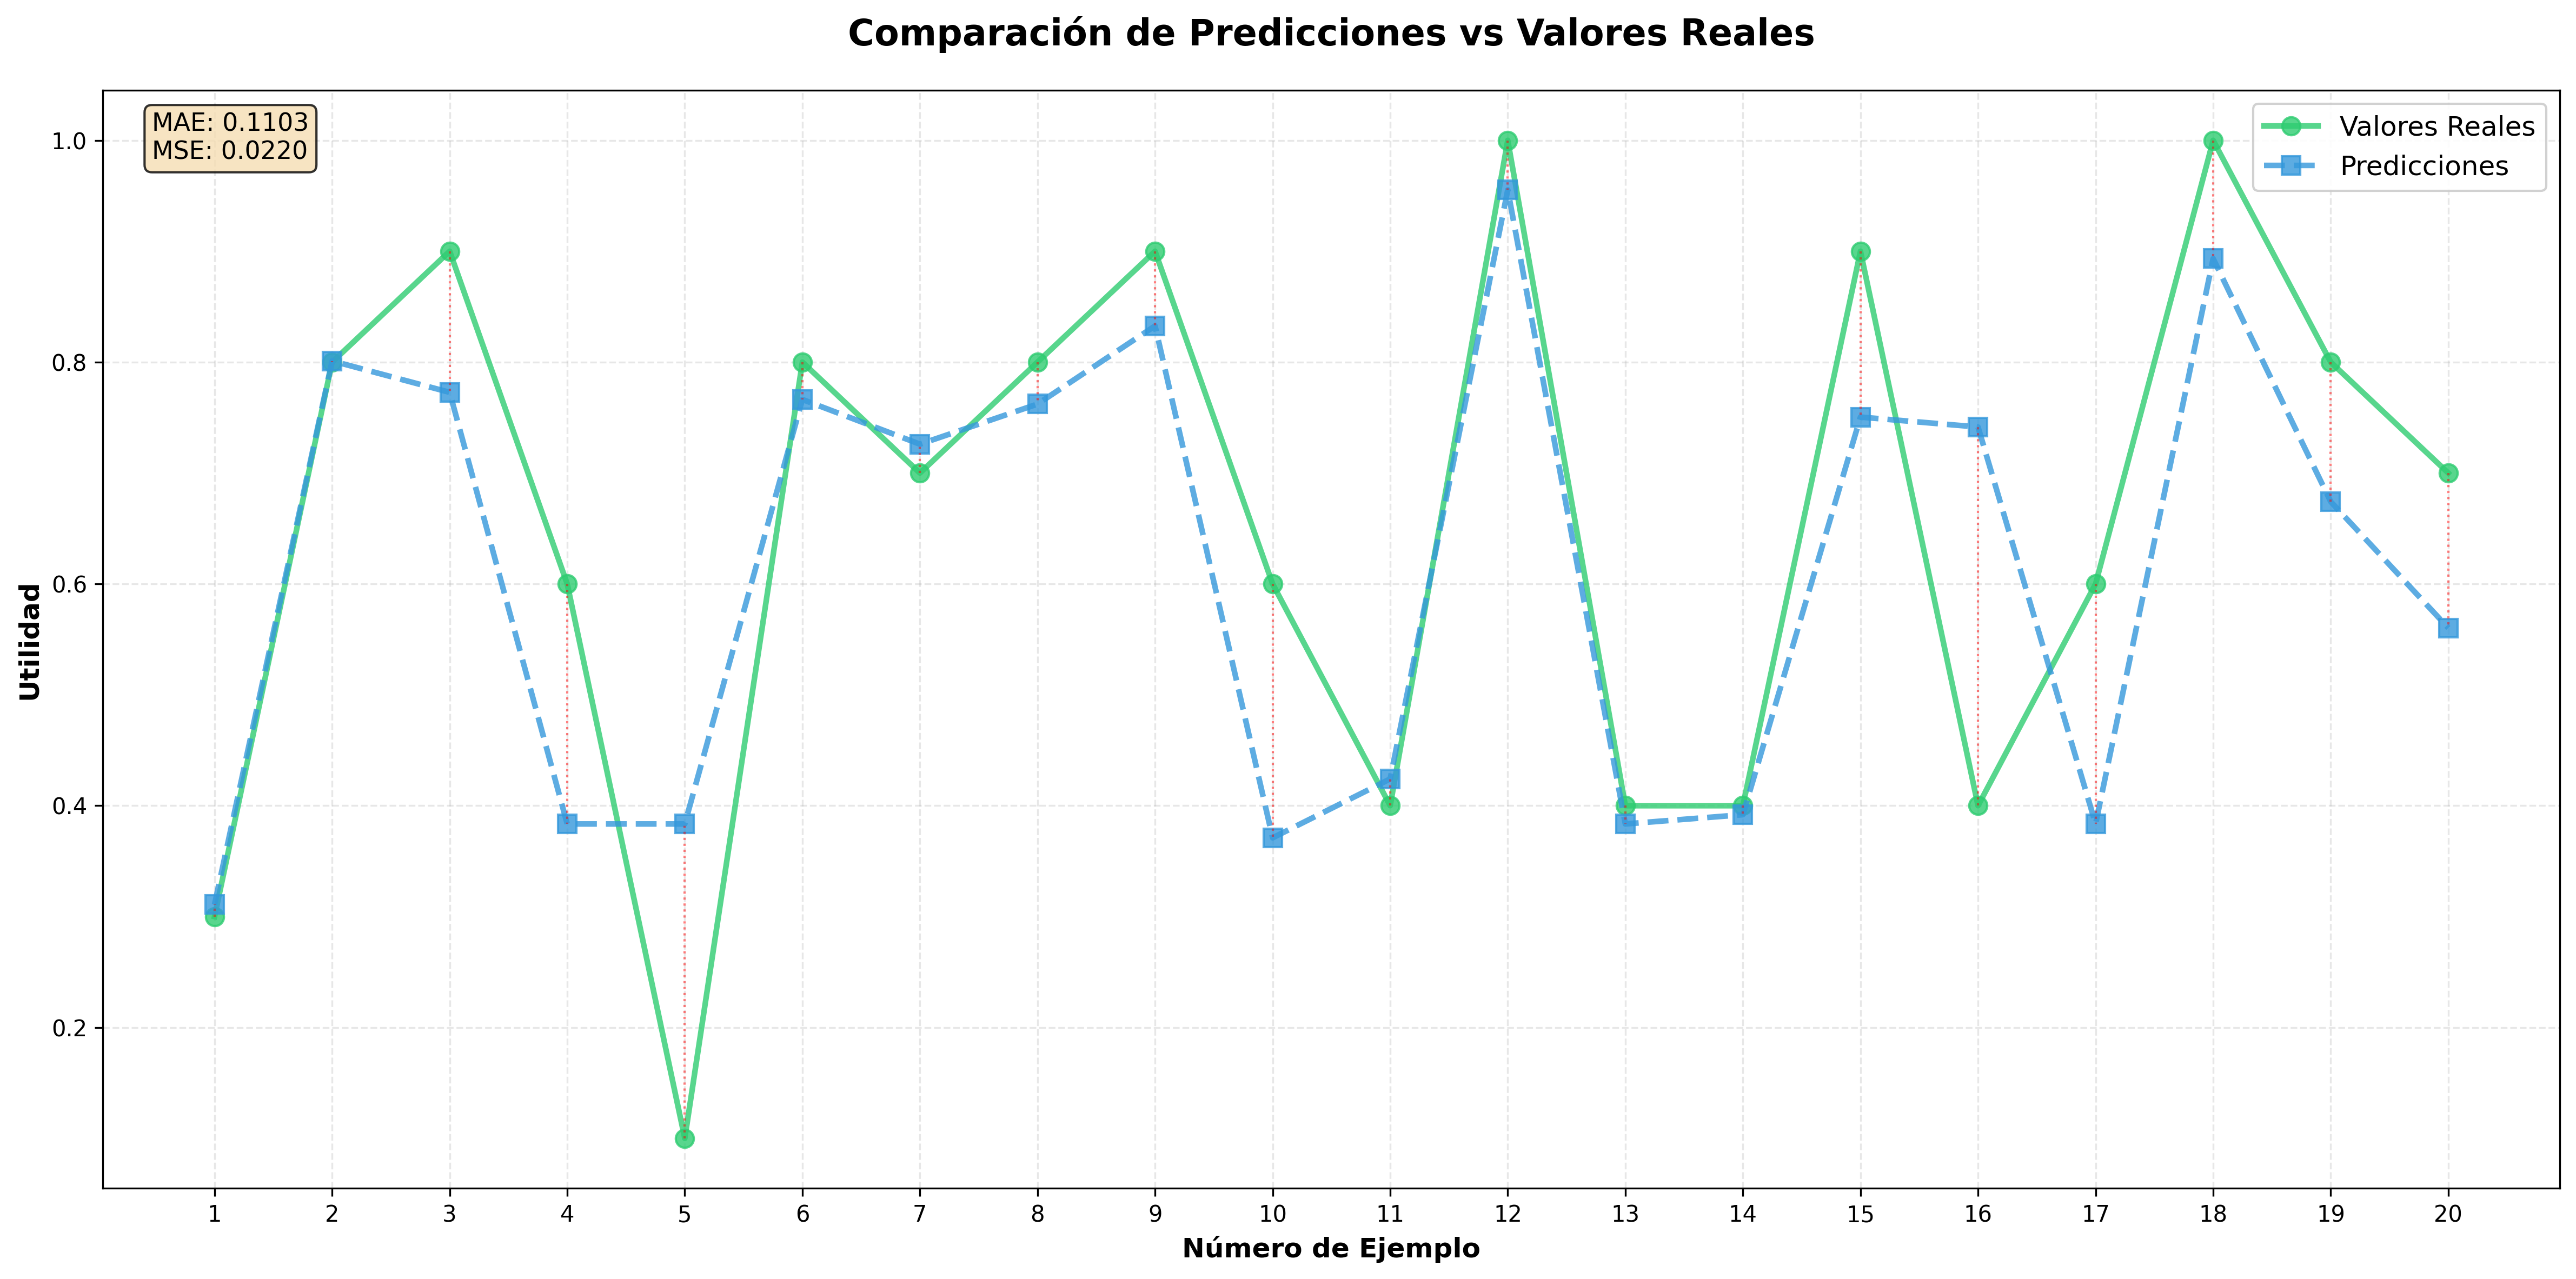
\includegraphics[width=\textwidth]{imaxes/UM/UM_predicciones_100.png}
  \caption{Predicciones del modelo de utilidad.}
  \label{fig:UM_predicciones_100}
\end{figure}

En conclusión, los resultados de las gráficas demuestran que el modelo de utilidad cumple con su función: evaluar cada estado en función de lo favorable que resulta para alcanzar un objetivo 
concreto. El resultado de esta fase permitió formalizar computacionalmente el objetivo del sistema, en lugar de programar directamente este objetivo, el sistema debía aprender por su cuenta 
una función que evaluará la utilidad de los estados.

\subsection{Demostración del sistema deliberativo}
\label{sec:desarrollo_demostracion_sistema}

Una vez completado el entrenamiento de los modelos de mundo y de utilidad, se procedió a validar el funcionamiento conjunto de ambos mediante una demostración en el entorno real. Para esto, 
se desarrolló un \gls{script} de demostración, que buscaba actuar como prueba final del trabajo realizado, combinando las percepciones obtenidas mediante el sistema Optitrack, el repertorio de 
acciones del robot y los modelos entrenados para tomar decisiones.

El funcionamiento sigue la lógica planteada desde el inicio del proyecto: En cada iteración, el sistema obtiene las observaciones actuales del entorno y genera, para cada una de las 9 acciones 
disponibles, la predicción del estado siguiente utilizando el modelo de mundo. Tras esto, el modelo de utilidad evalúa cada uno de los estados predichos, obteniendo así la estimación de su 
utilidad para lograr el objetivo. Finalmente, el sistema selecciona la acción asociada a la observación con mayor valor de utilidad y la ejecuta en el robot.

En la figura \ref{fig:iteracion_demostracion} se muestra un ejemplo de una iteración de la ejecución de este \gls{script} de demostración del sistema deliberativo en la que se aprecia el 
funcionamiento de este: a partir de la observación actual, utiliza el modelo de mundo para predecir el estado siguiente para cada una de las acciones. Tras esto, evalúa cada uno de estos 
estados mediante el modelo de utilidad y selecciona la acción que proporciona mayor valor de utilidad.

\begin{figure}[hp!]
  \centering
  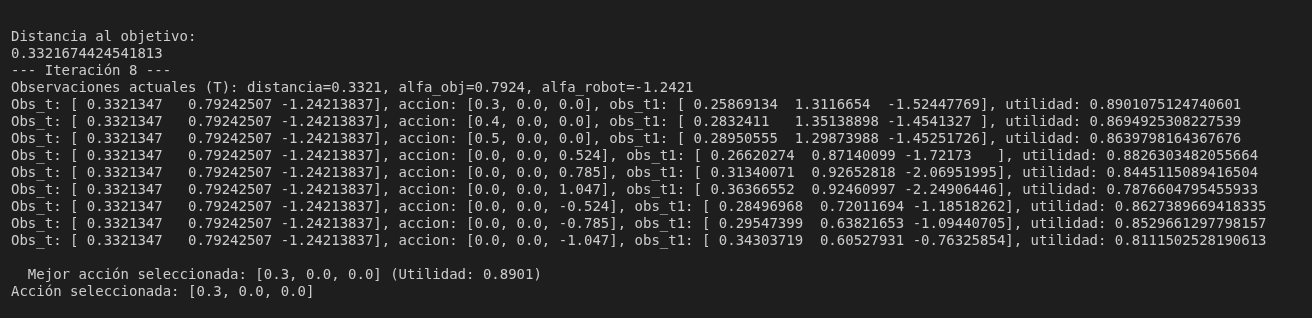
\includegraphics[width=\textwidth]{imaxes/Captura_IteracionDemostracion.png}
  \caption{Ejemplo de una iteración del sistema deliberativo.}
  \label{fig:iteracion_demostracion}
\end{figure}

La figura \ref{fig:Secuencia_ejecucion_sistema} presenta una secuencia de imágenes capturadas durante una ejecución real del sistema. En ellas se puede observar el recorrido que sigue el 
robot, acercándose cada vez más al objetivo, hasta alcanzarlo finalmente. Cada una de las distintas capturas se corresponde con una iteración y representa el instante tras haber ejecutado 
una acción. A través de esta secuencia se puede observar como el sistema es capaz de cumplir con el objetivo planteado combinando los modelos de mundo y de utilidad.

\begin{figure}[hp!]
  \centering

  \begin{subfigure}[c]{0.45\textwidth}
    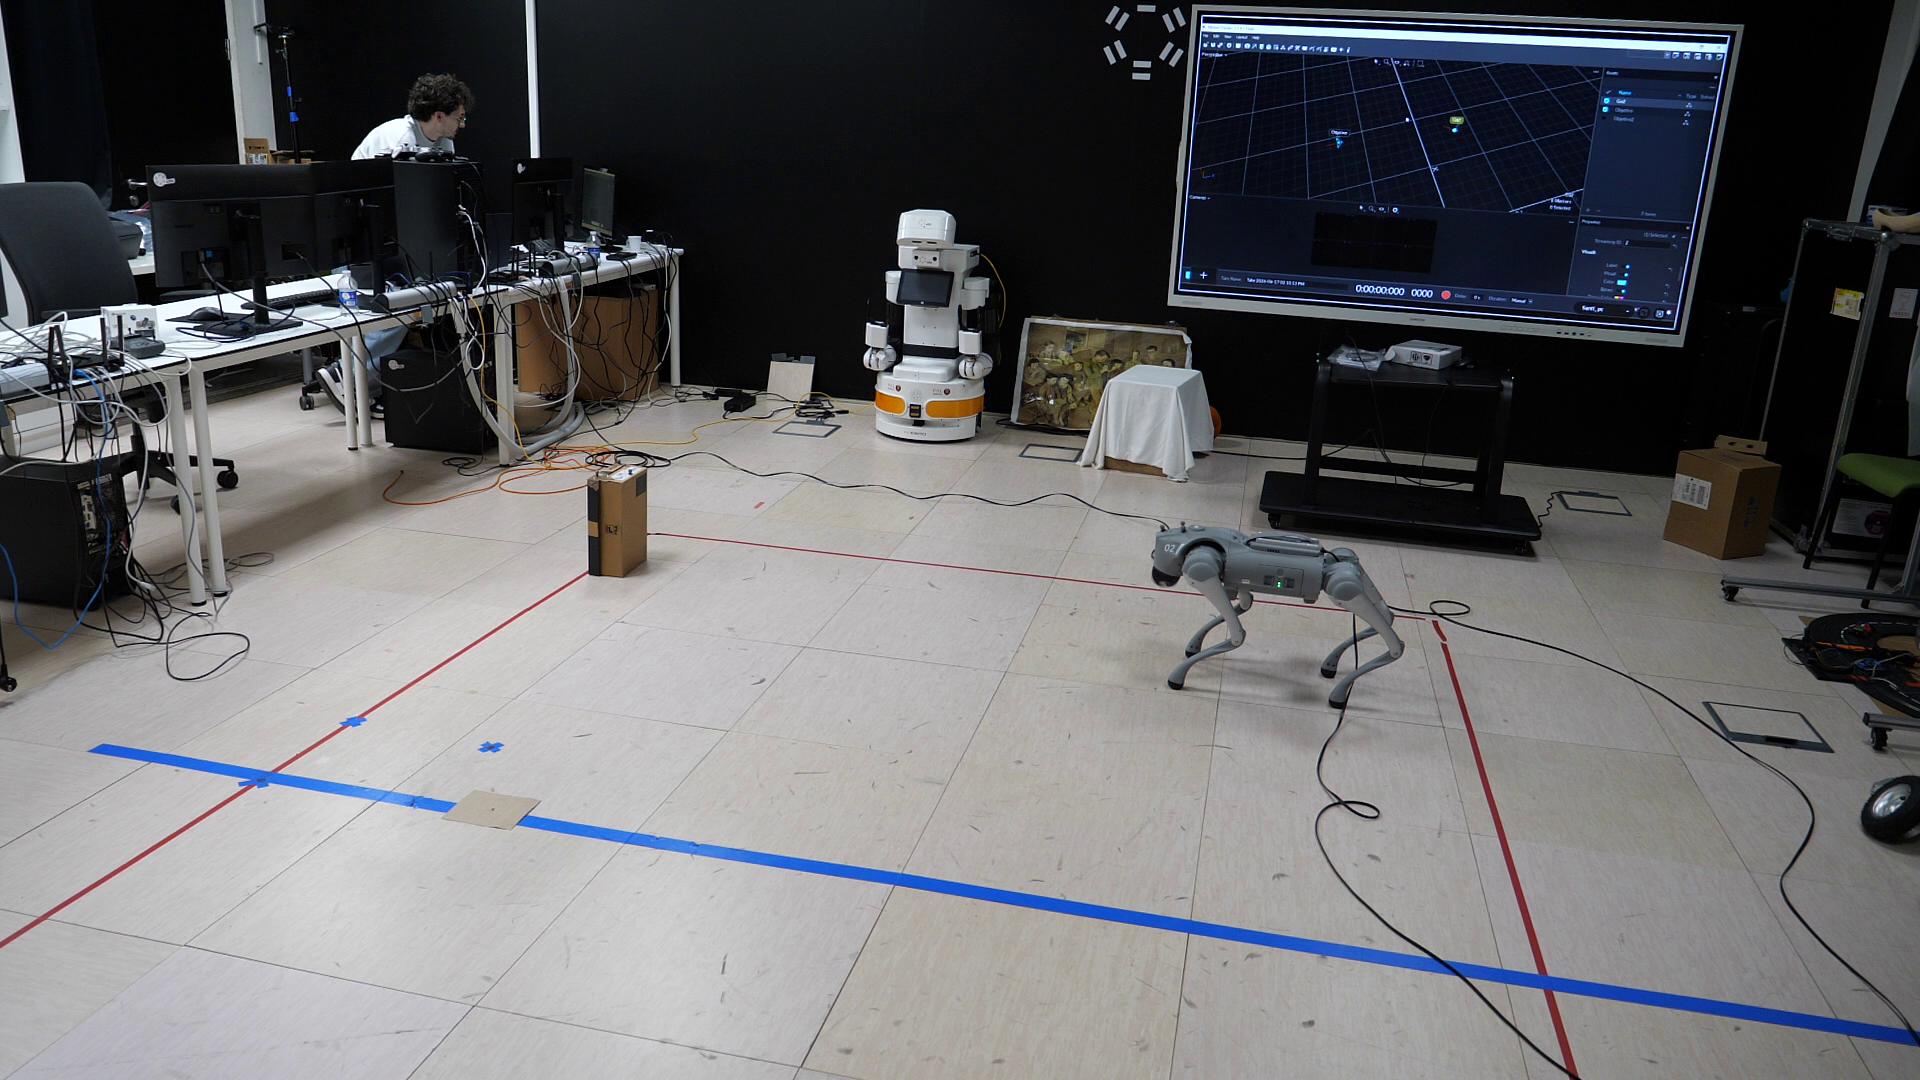
\includegraphics[width=\textwidth]{imaxes/CapturasVideo1/Captura1.1.png}
    \caption{Captura 1.}
    \label{fig:Secuencia_ejecucion_sistema_1}
  \end{subfigure}
  \hfill
  \begin{subfigure}[c]{0.45\textwidth}
    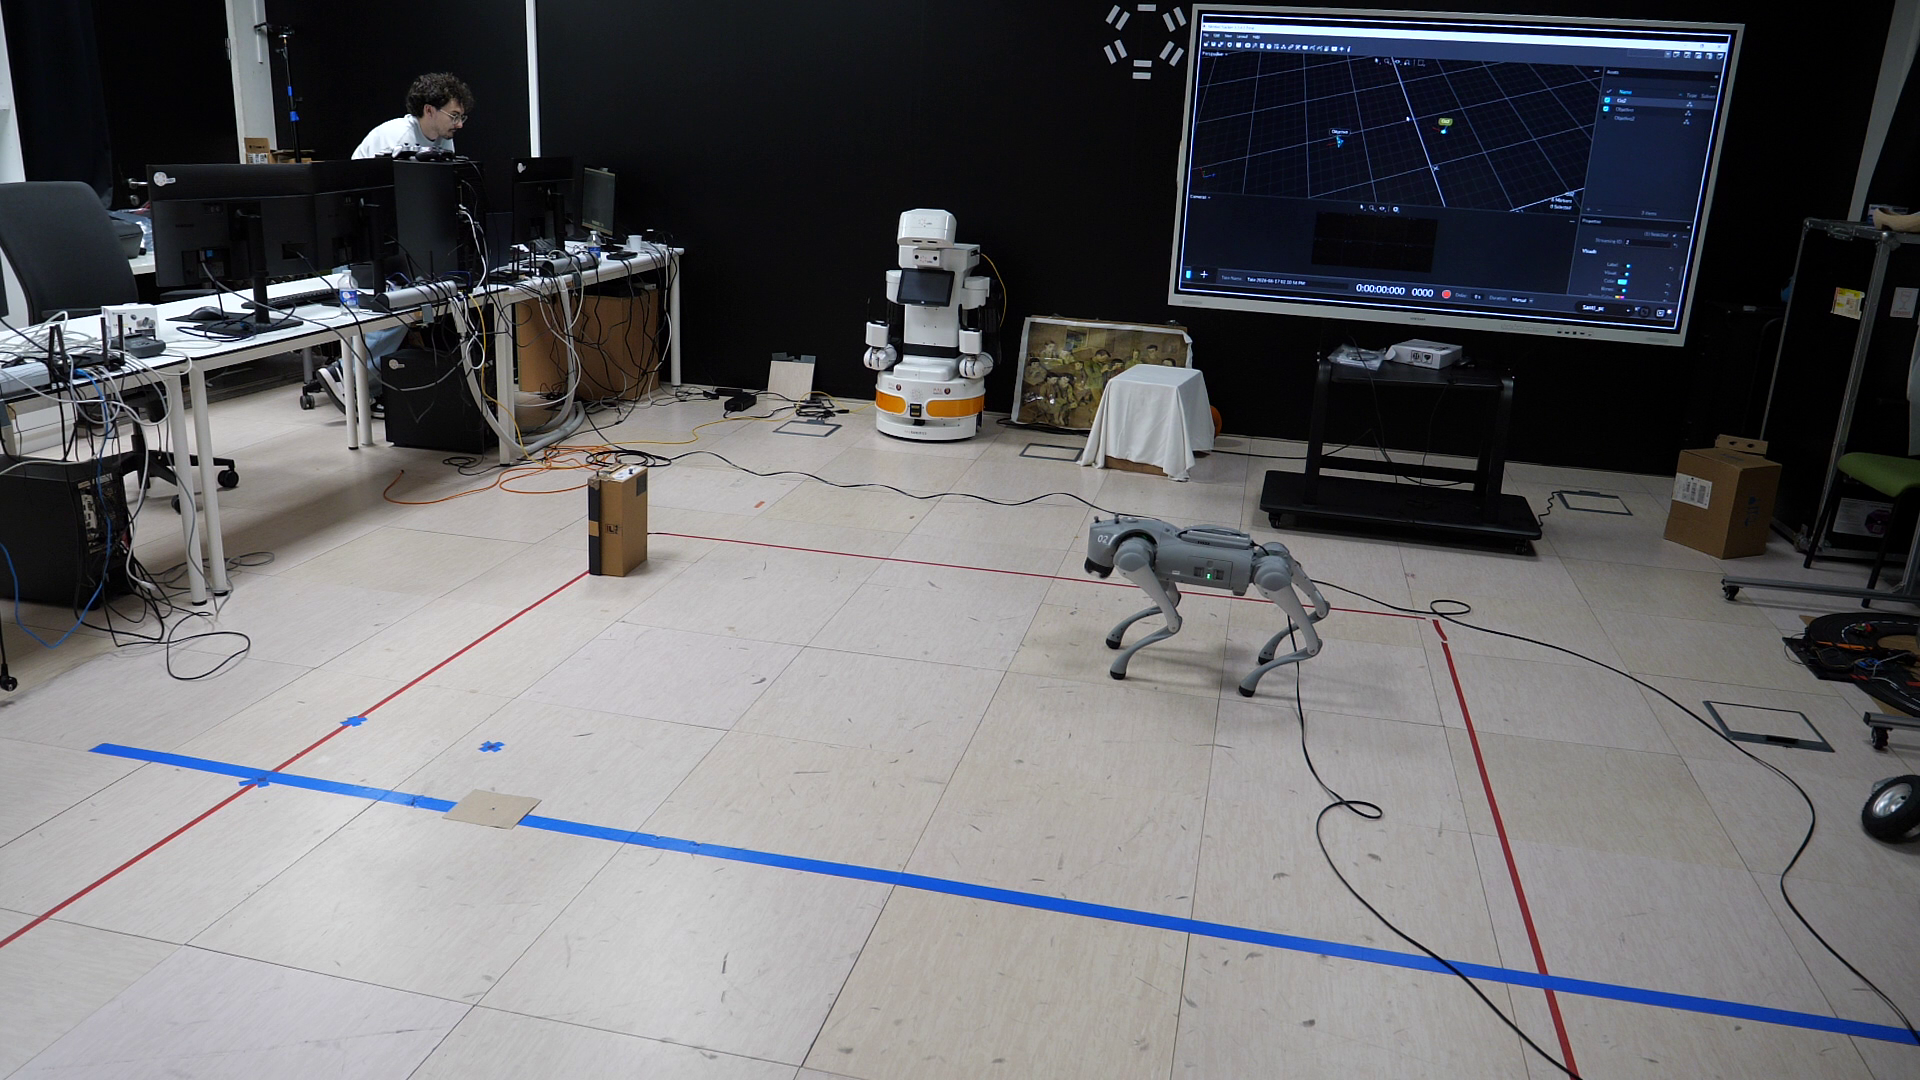
\includegraphics[width=\textwidth]{imaxes/CapturasVideo1/Captura1.2.png}
    \caption{Captura 2.}
    \label{fig:Secuencia_ejecucion_sistema_2}
  \end{subfigure}

  \vspace{0.4cm}

  \begin{subfigure}[c]{0.45\textwidth}
    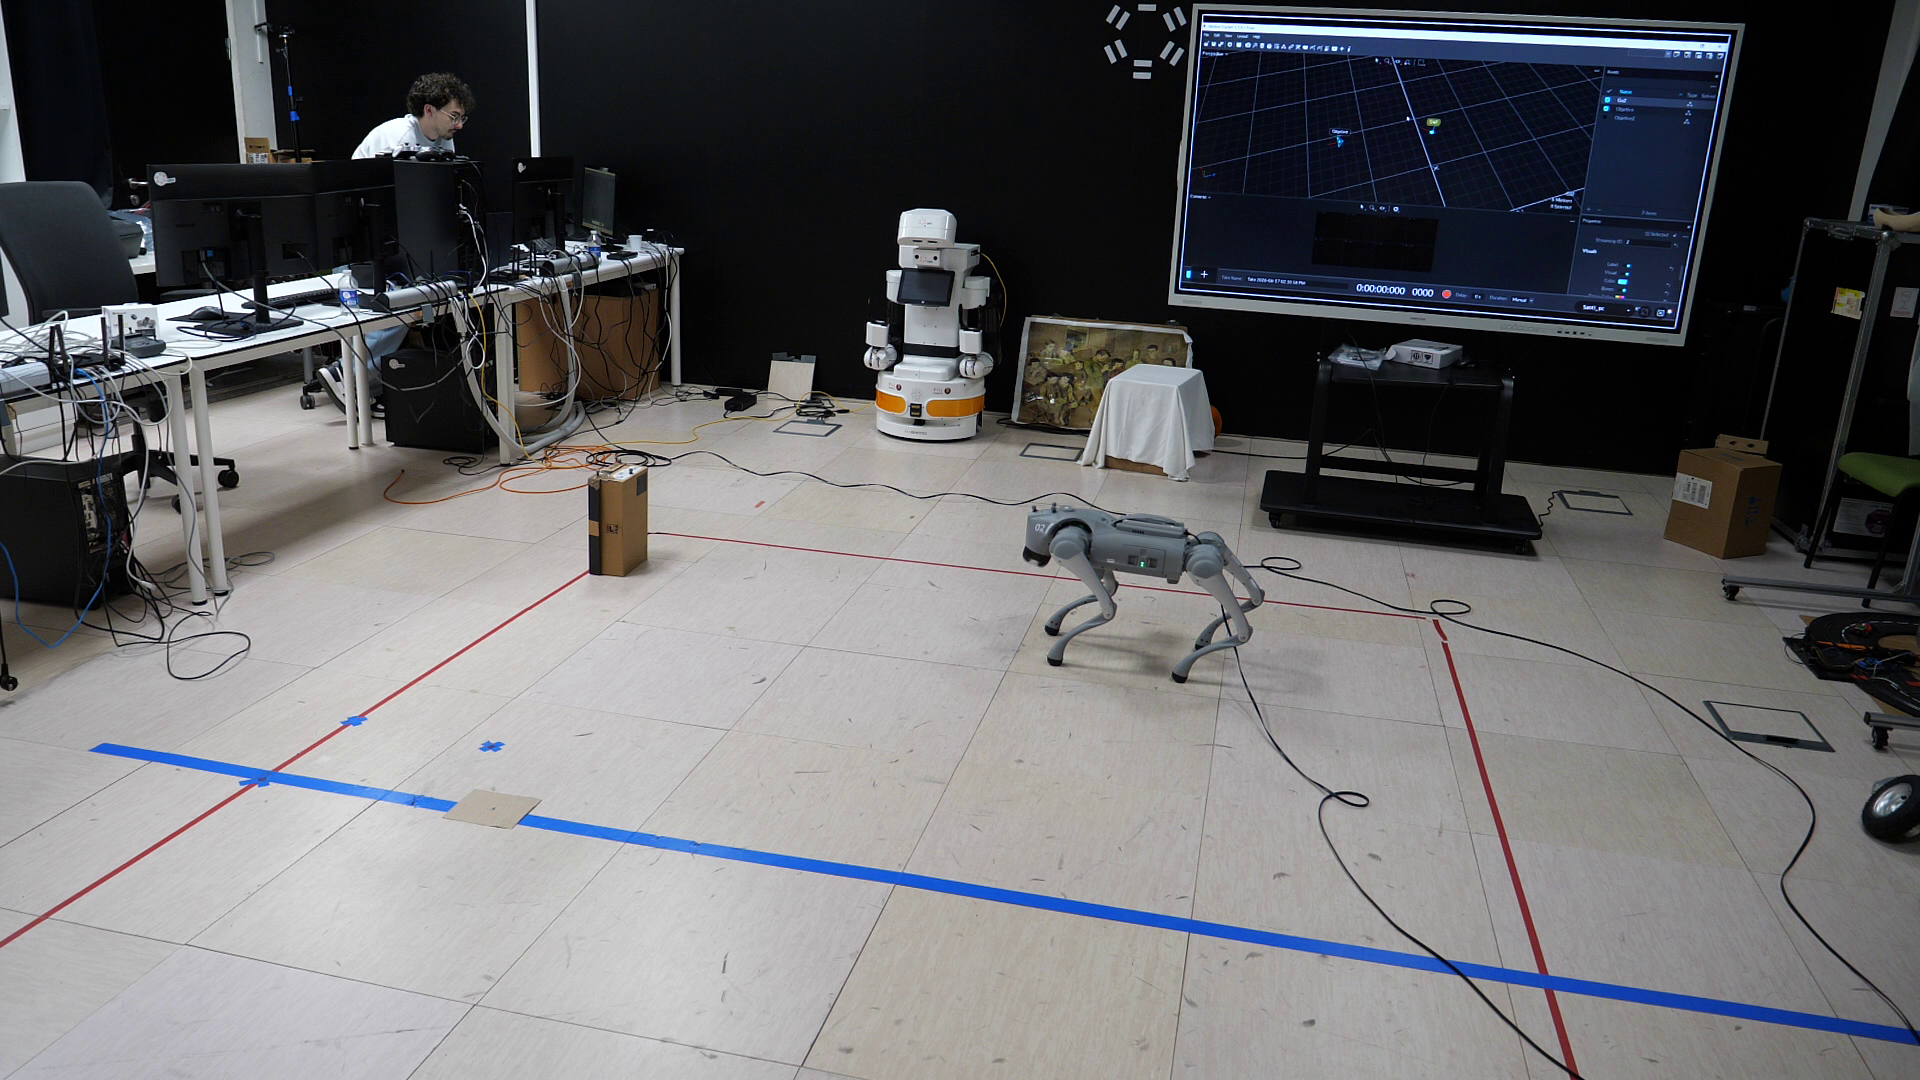
\includegraphics[width=\textwidth]{imaxes/CapturasVideo1/Captura1.3.png}
    \caption{Captura 3.}
    \label{fig:Secuencia_ejecucion_sistema_3}
  \end{subfigure}
  \hfill
  \begin{subfigure}[c]{0.45\textwidth}
    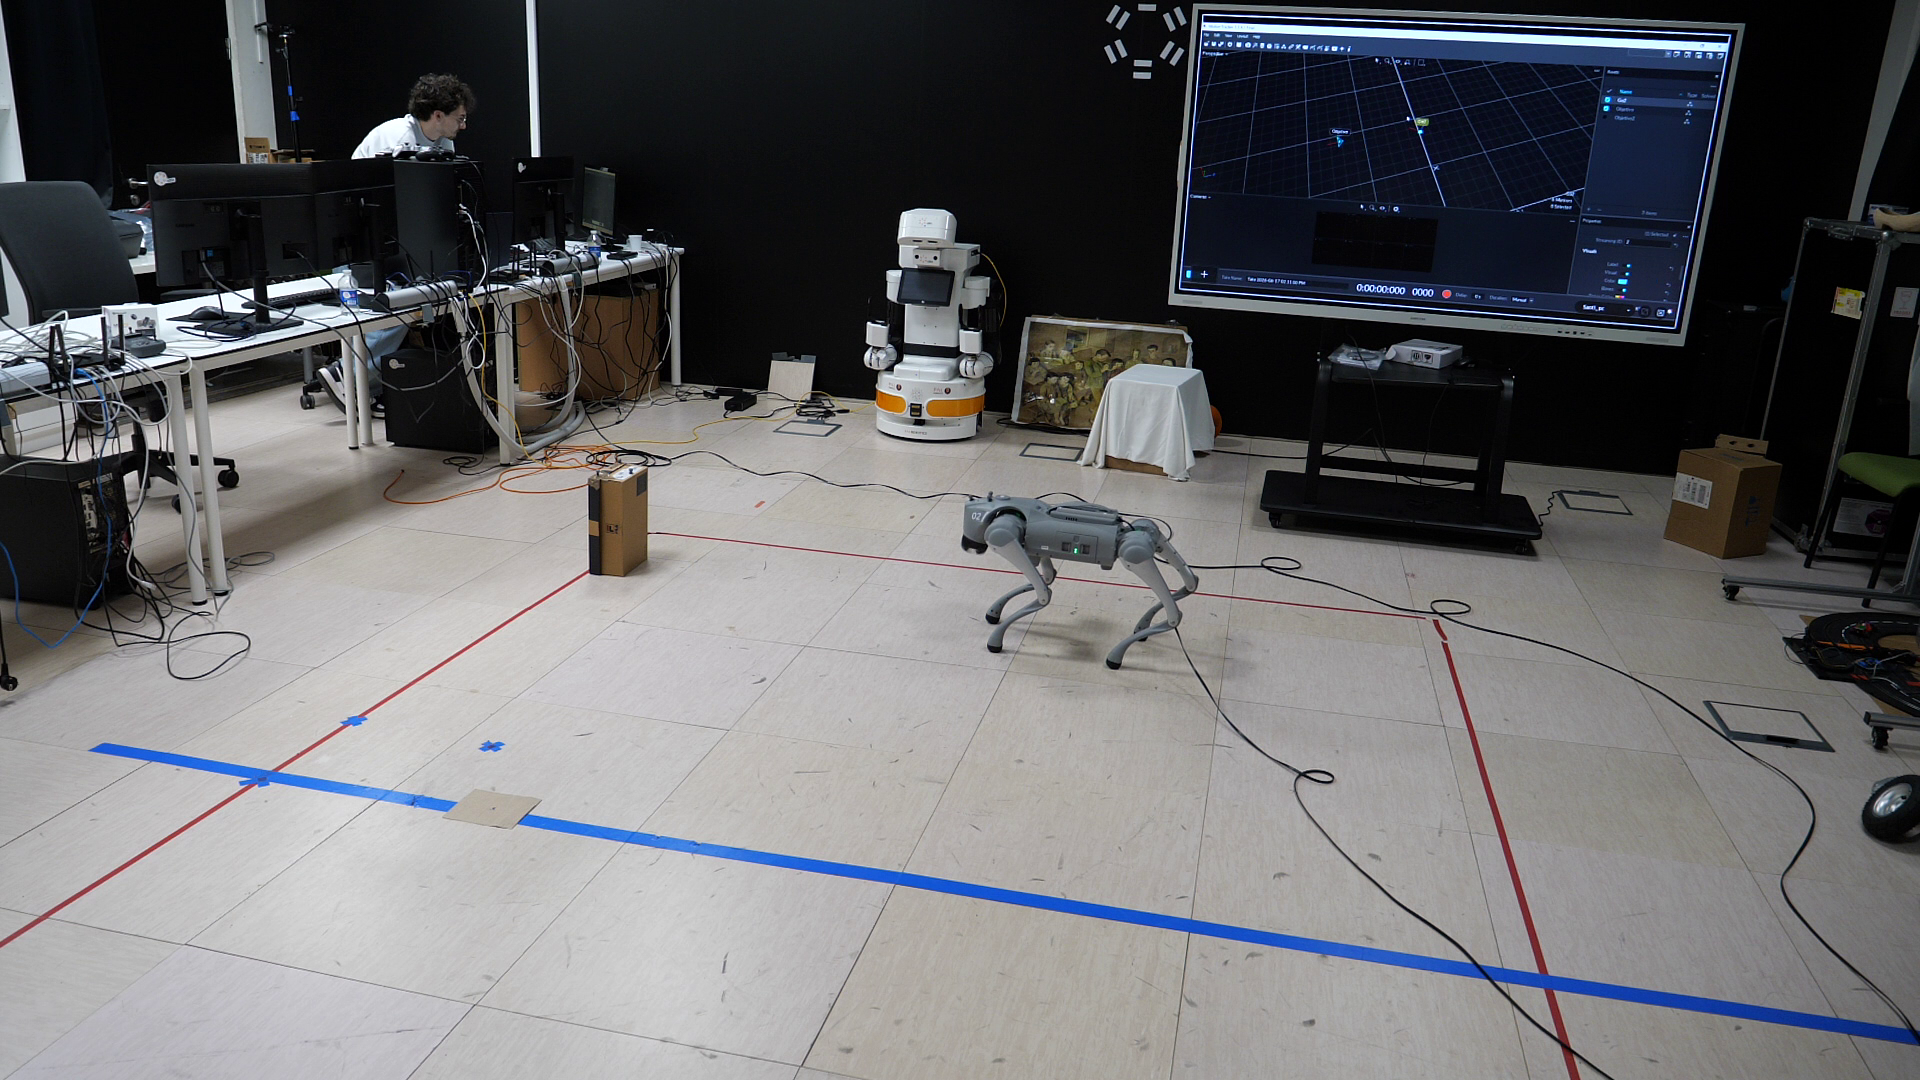
\includegraphics[width=\textwidth]{imaxes/CapturasVideo1/Captura1.4.png}
    \caption{Captura 4.}
    \label{fig:Secuencia_ejecucion_sistema_4}
  \end{subfigure}

  \vspace{0.4cm}

  \begin{subfigure}[c]{0.45\textwidth}
    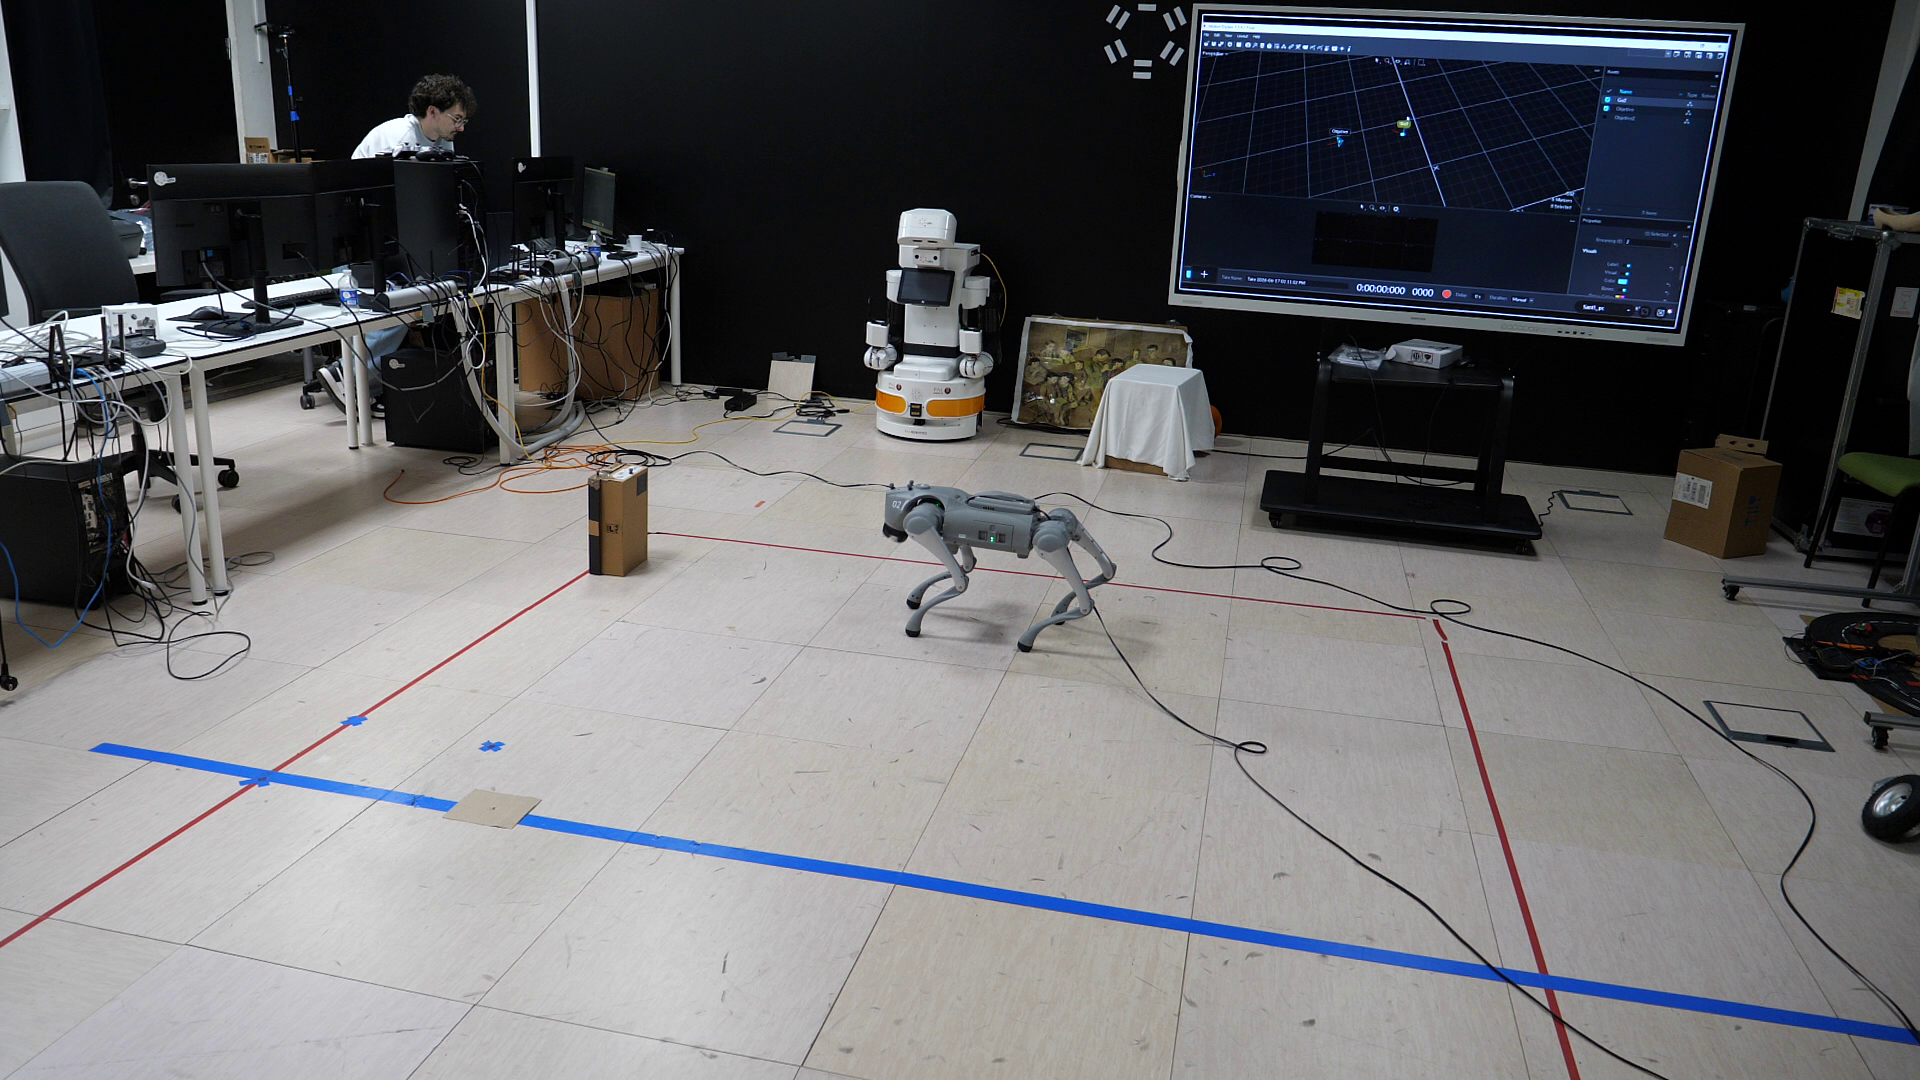
\includegraphics[width=\textwidth]{imaxes/CapturasVideo1/Captura1.5.png}
    \caption{Captura 5.}
    \label{fig:Secuencia_ejecucion_sistema_5}
  \end{subfigure}
  \hfill
  \begin{subfigure}[c]{0.45\textwidth}
    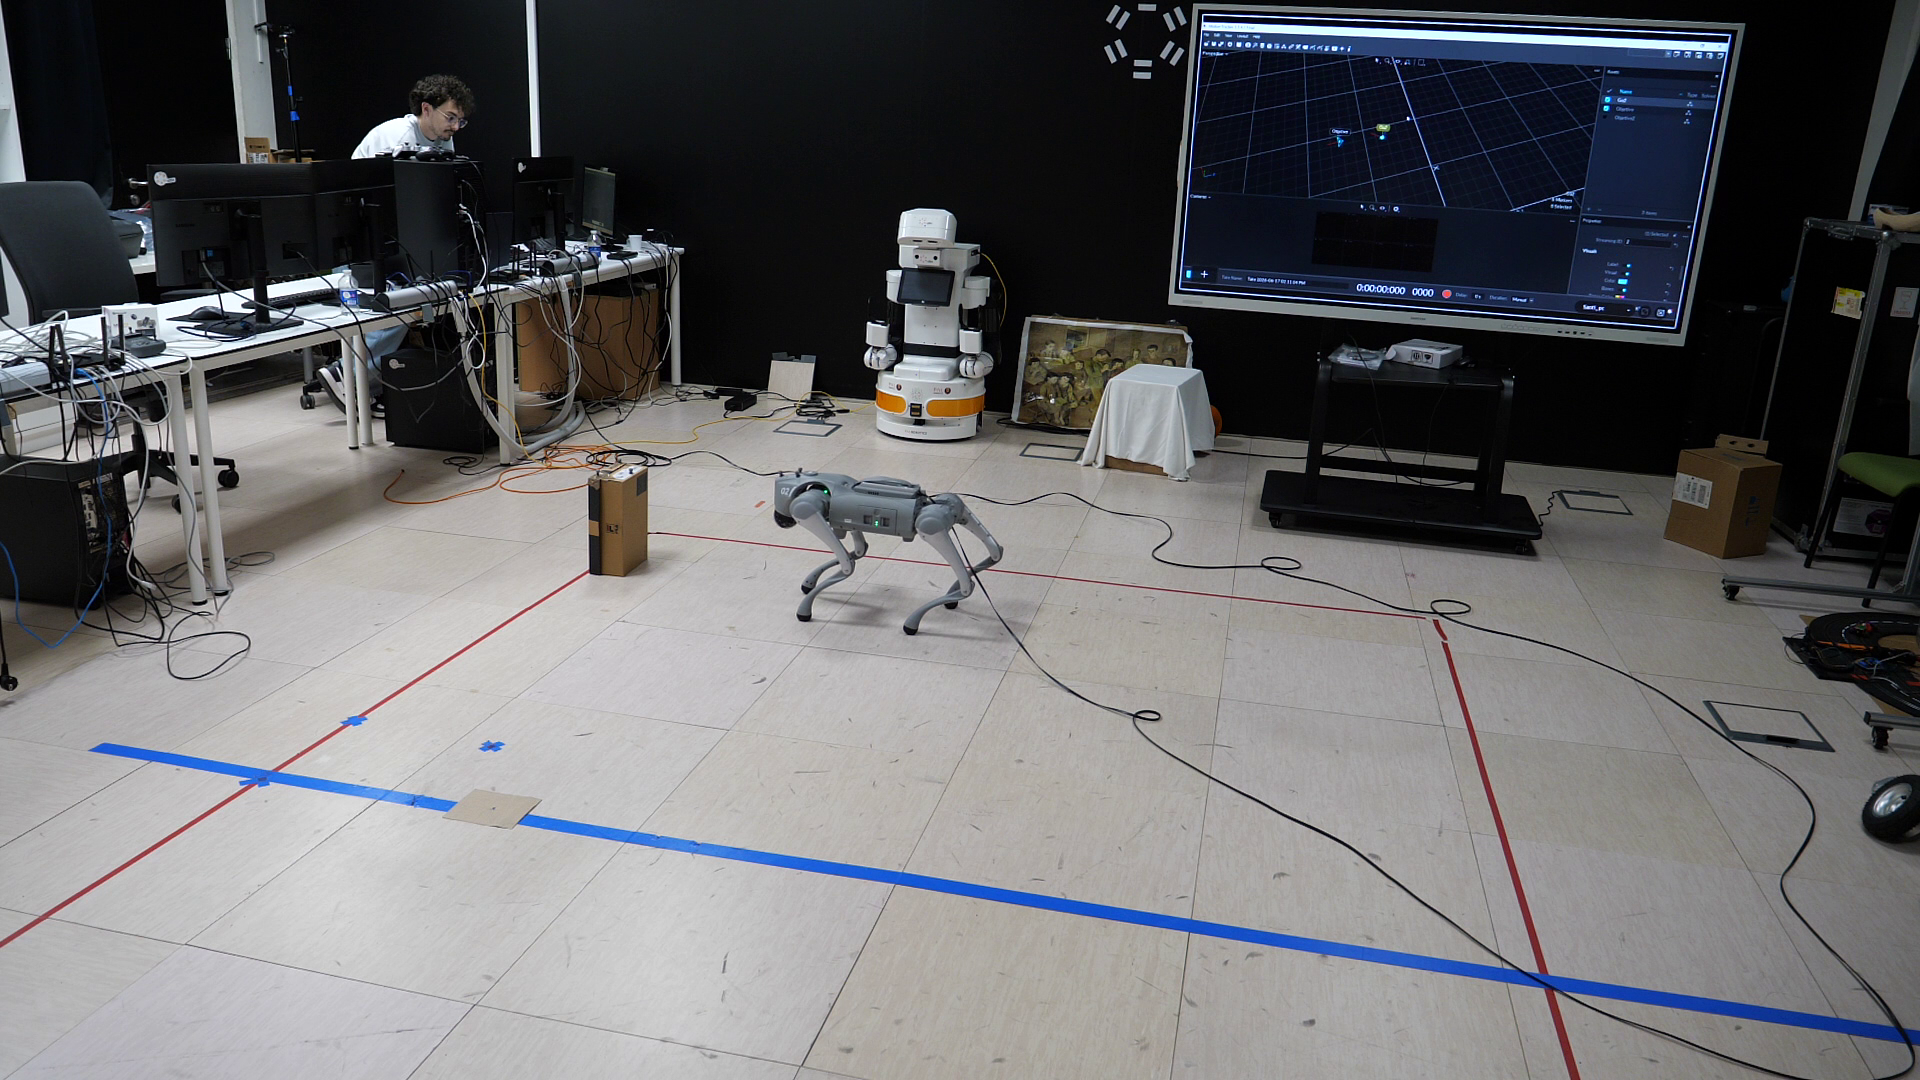
\includegraphics[width=\textwidth]{imaxes/CapturasVideo1/Captura1.6.png}
    \caption{Captura 6.}
    \label{fig:Secuencia_ejecucion_sistema_6}
  \end{subfigure}

  \vspace{0.4cm}

  \begin{subfigure}[c]{0.45\textwidth}
    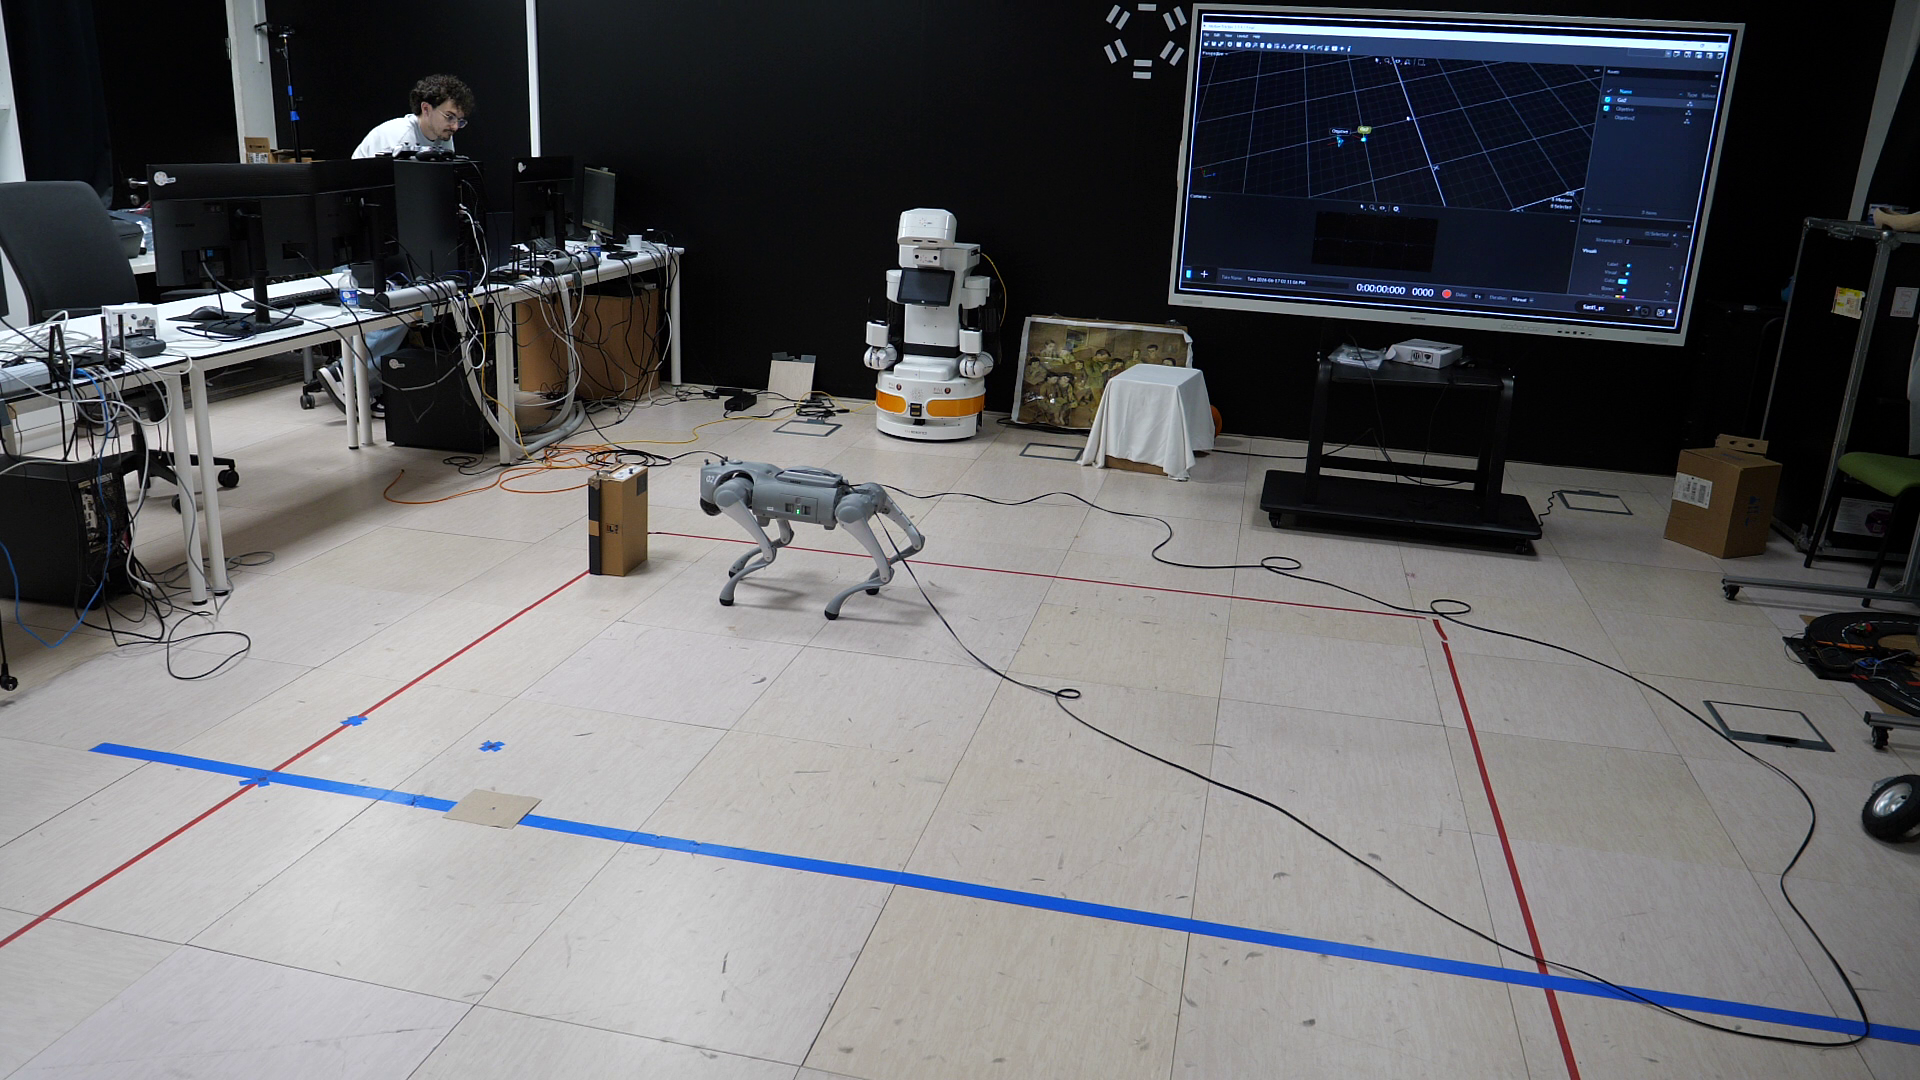
\includegraphics[width=\textwidth]{imaxes/CapturasVideo1/Captura1.7.png}
    \caption{Captura 7.}
    \label{fig:Secuencia_ejecucion_sistema_7}
  \end{subfigure}
  \hfill
  \begin{subfigure}[c]{0.45\textwidth}
    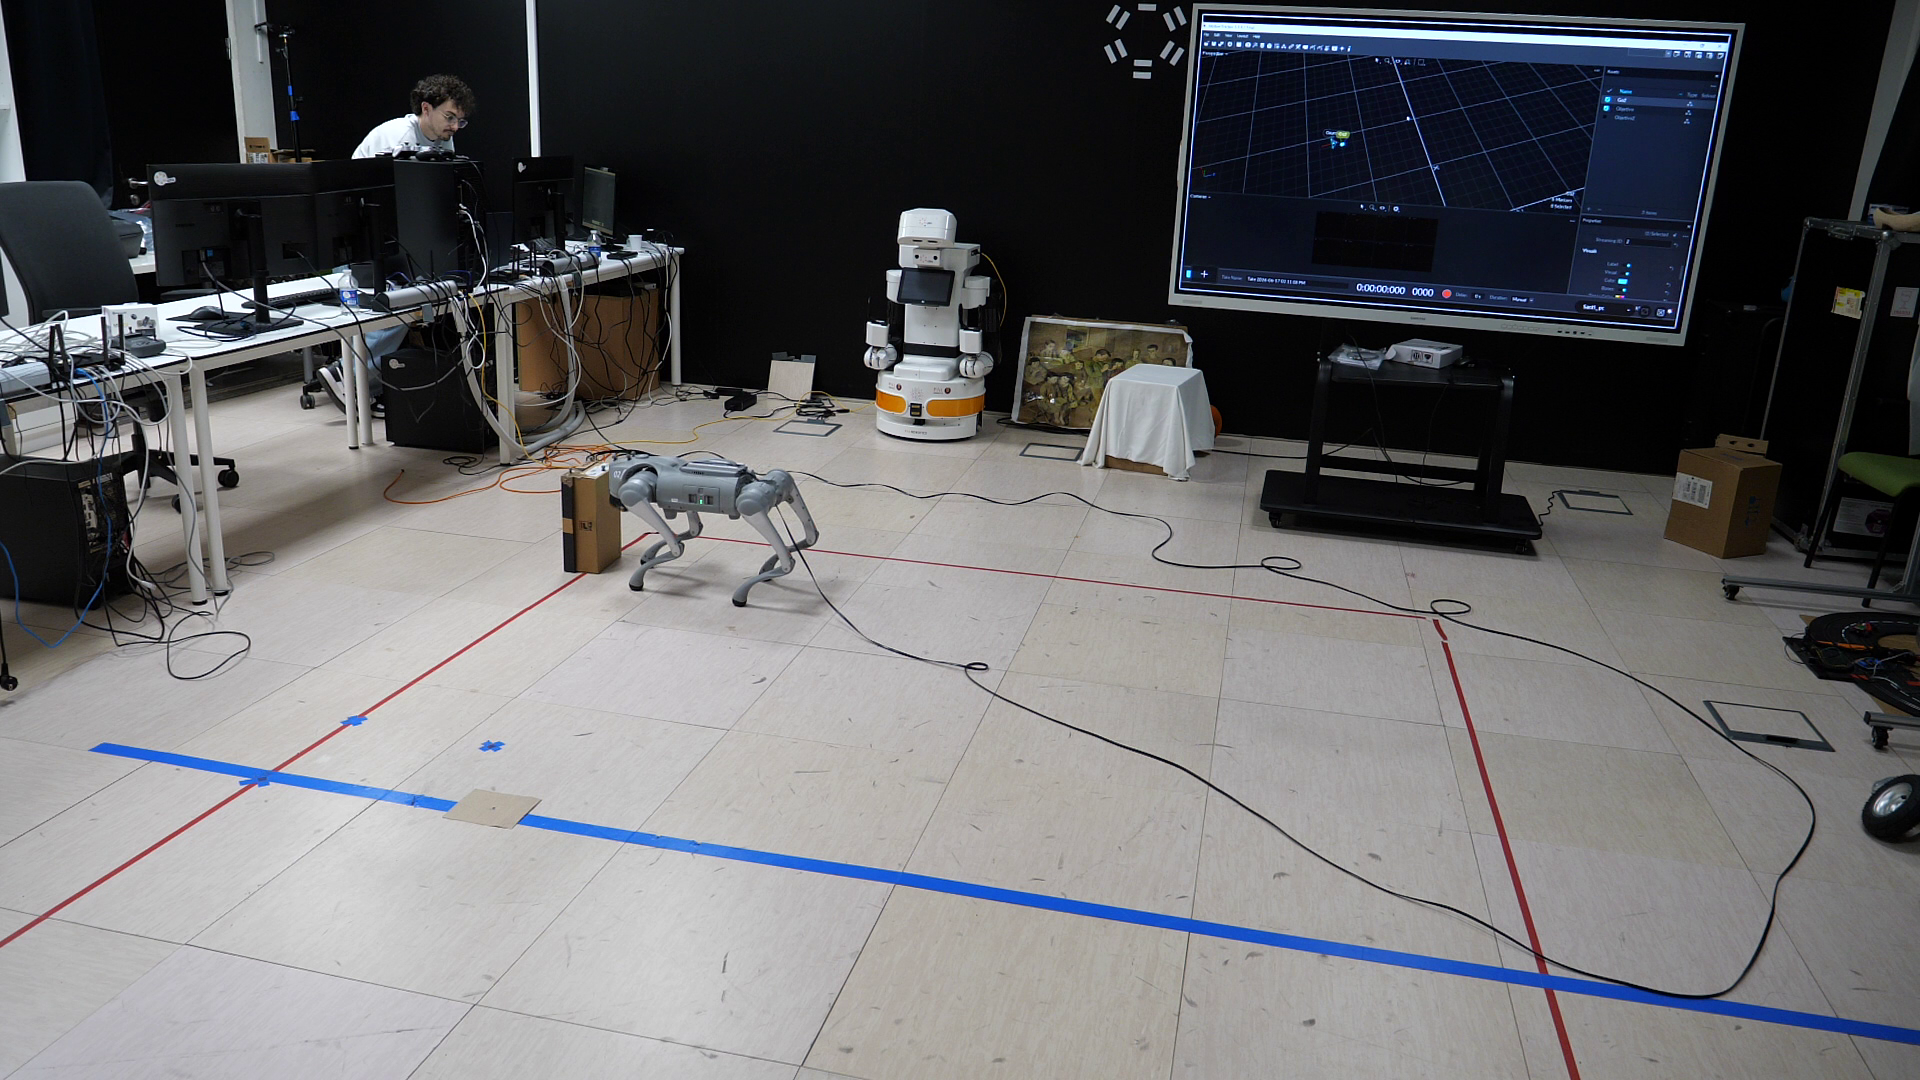
\includegraphics[width=\textwidth]{imaxes/CapturasVideo1/Captura1.8.png}
    \caption{Captura 8.}
    \label{fig:Secuencia_ejecucion_sistema_8}
  \end{subfigure}

  \caption{Secuencia de imagenes de una ejecución del sistema deliberativo.}
  \label{fig:Secuencia_ejecucion_sistema}
\end{figure}

Por último, en la figura \ref{fig:grafica_relacion_ut_dist} se muestra la relación entre los valores de utilidad estimados y la distancia con el objetivo a lo largo de varias iteraciones. Esta 
gráfica se extrae de la ejecución vista anteriormente en la figura \ref{fig:Secuencia_ejecucion_sistema}. En ella se observa cómo, a medida que el robot se aproxima al objetivo y la distancia 
disminuye, la utilidad aumenta. Este comportamiento confirma que el modelo ha sido capaz de aprender la relación entre las observaciones del entorno y la utilidad de estas para alcanzar la meta.

\begin{figure}[hp!]
  \centering
  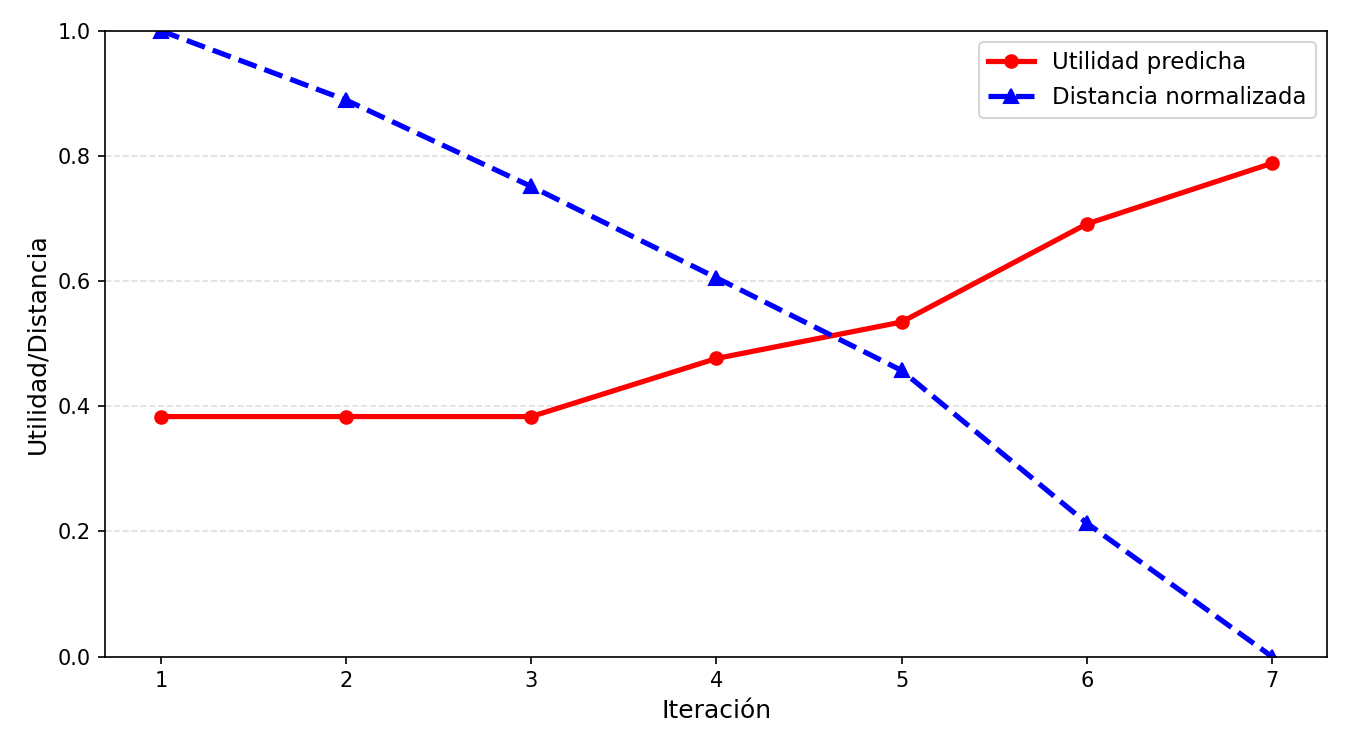
\includegraphics[width=0.75\textwidth]{imaxes/grafica_relacion_ut_dist_1.png}
  \caption{Gráfica de la relación entre la utilidad y la distancia para cada iteración.}
  \label{fig:grafica_relacion_ut_dist}
\end{figure}

Los resultados obtenidos durante esta demostración permiten concluir que el sistema cumple con la idea principal propuesta para el trabajo: crear un sistema de toma de decisiones deliberativo 
que se basa en un modelo de mundo que predice las consecuencias de una acción y en un modelo de utilidad que valora esas consecuencias antes de actuar. Además, su finalización permite validar 
que el enfoque utilizado era funcional incluso tras haber eliminado la fase de simulación.


\subsection{Independencia entre modelos}
\label{sec:desarrollo_indep_mod}

Otro de los puntos que buscaba demostrar este trabajo es la independencia entre modelos de mundo y modelos de utilidad. Esta independencia es un aspecto importante del sistema, ya que permite 
separar las predicciones de los estados del entorno de la evaluación de estos mismos. Siguiendo esta idea, debería ser posible sustituir uno de ellos manteniendo el otro, siempre y cuando, las 
entradas y las salidas continúen siendo compatibles (es decir, cuando las observaciones sean las mismas).

Para probar esto, se realizaron dos pruebas diferentes: En la primera se mantuvo el modelo de mundo del robot Unitree Go2 y se sustituyó el modelo de utilidad por otro entrenado para cumplir 
n objetivo distinto, en este caso alejarse de un objeto. En la segunda se mantuvo el modelo de utilidad original y se sustituyó el modelo de mundo del Go2 por otro correspondiente a un dominio 
distinto, una simulación sencilla de un brazo robótico en 2D.


\subsubsection{Mismo modelo de mundo, diferente modelo de utilidad}

En primer lugar, se comprobó si el modelo de mundo entrenado para el Go2 podía funcionar con un modelo de utilidad diferente. El modelo de mundo había aprendido cómo cambian las observaciones 
en el entorno real en función de la acción ejecutada. Por tanto, el modelo no depende directamente de la meta, sino de la relación entre el estado, la acción y el estado siguiente.

Para comprobar esta premisa, se entrenó un modelo de utilidad cuyo objetivo era alejarse del objetivo. Mientras que el modelo original valoraba positivamente las posiciones cercanas al objetivo, 
este nuevo modelo buscaba asignar mayor utilidad a los estados más alejados. Esto se realizó así para reutilizar el conjunto de datos anterior, invirtiendo los valores de utilidad asociados a 
cada observación, evitando así la parte más costosa de entrenar un nuevo modelo. De esta manera, las posiciones que antes recibían valores altos pasaron a obtener valores bajos, y viceversa. 
Además, al utilizar los datos originales, las entradas y salidas de los modelos continuaban siendo compatibles entre sí sin modificaciones.

El proceso de entrenamiento de este modelo de utilidad fue igual al empleado para el modelo original. Al contar con el conjunto de datos disponible desde un inicio, se saltó la parte de 
recolección y se pasó directamente al entrenamiento del modelo, empleando los parámetros utilizados anteriormente, como se puede apreciar en el apartado \ref{sec:desarrollo_UM}.

Los resultados obtenidos muestran que el modelo de utilidad fue capaz de aprender correctamente este nuevo objetivo. En la figura \ref{fig:UM_predicciones_100_inverso}, se muestra la comparación 
entre los valores reales y las predicciones realizadas por el modelo de algunos ejemplos. Aunque hay algunos pequeños errores presentes, la tendencia general se mantiene y las predicciones 
presentan los valores esperados. Además, las métricas de errores son reducidas, con un MAE de 0.1453 y un MSE de 0.0323, indicando que el modelo aproxima correctamente la utilidad para esta 
nueva meta.

\begin{figure}[hp!]
  \centering
  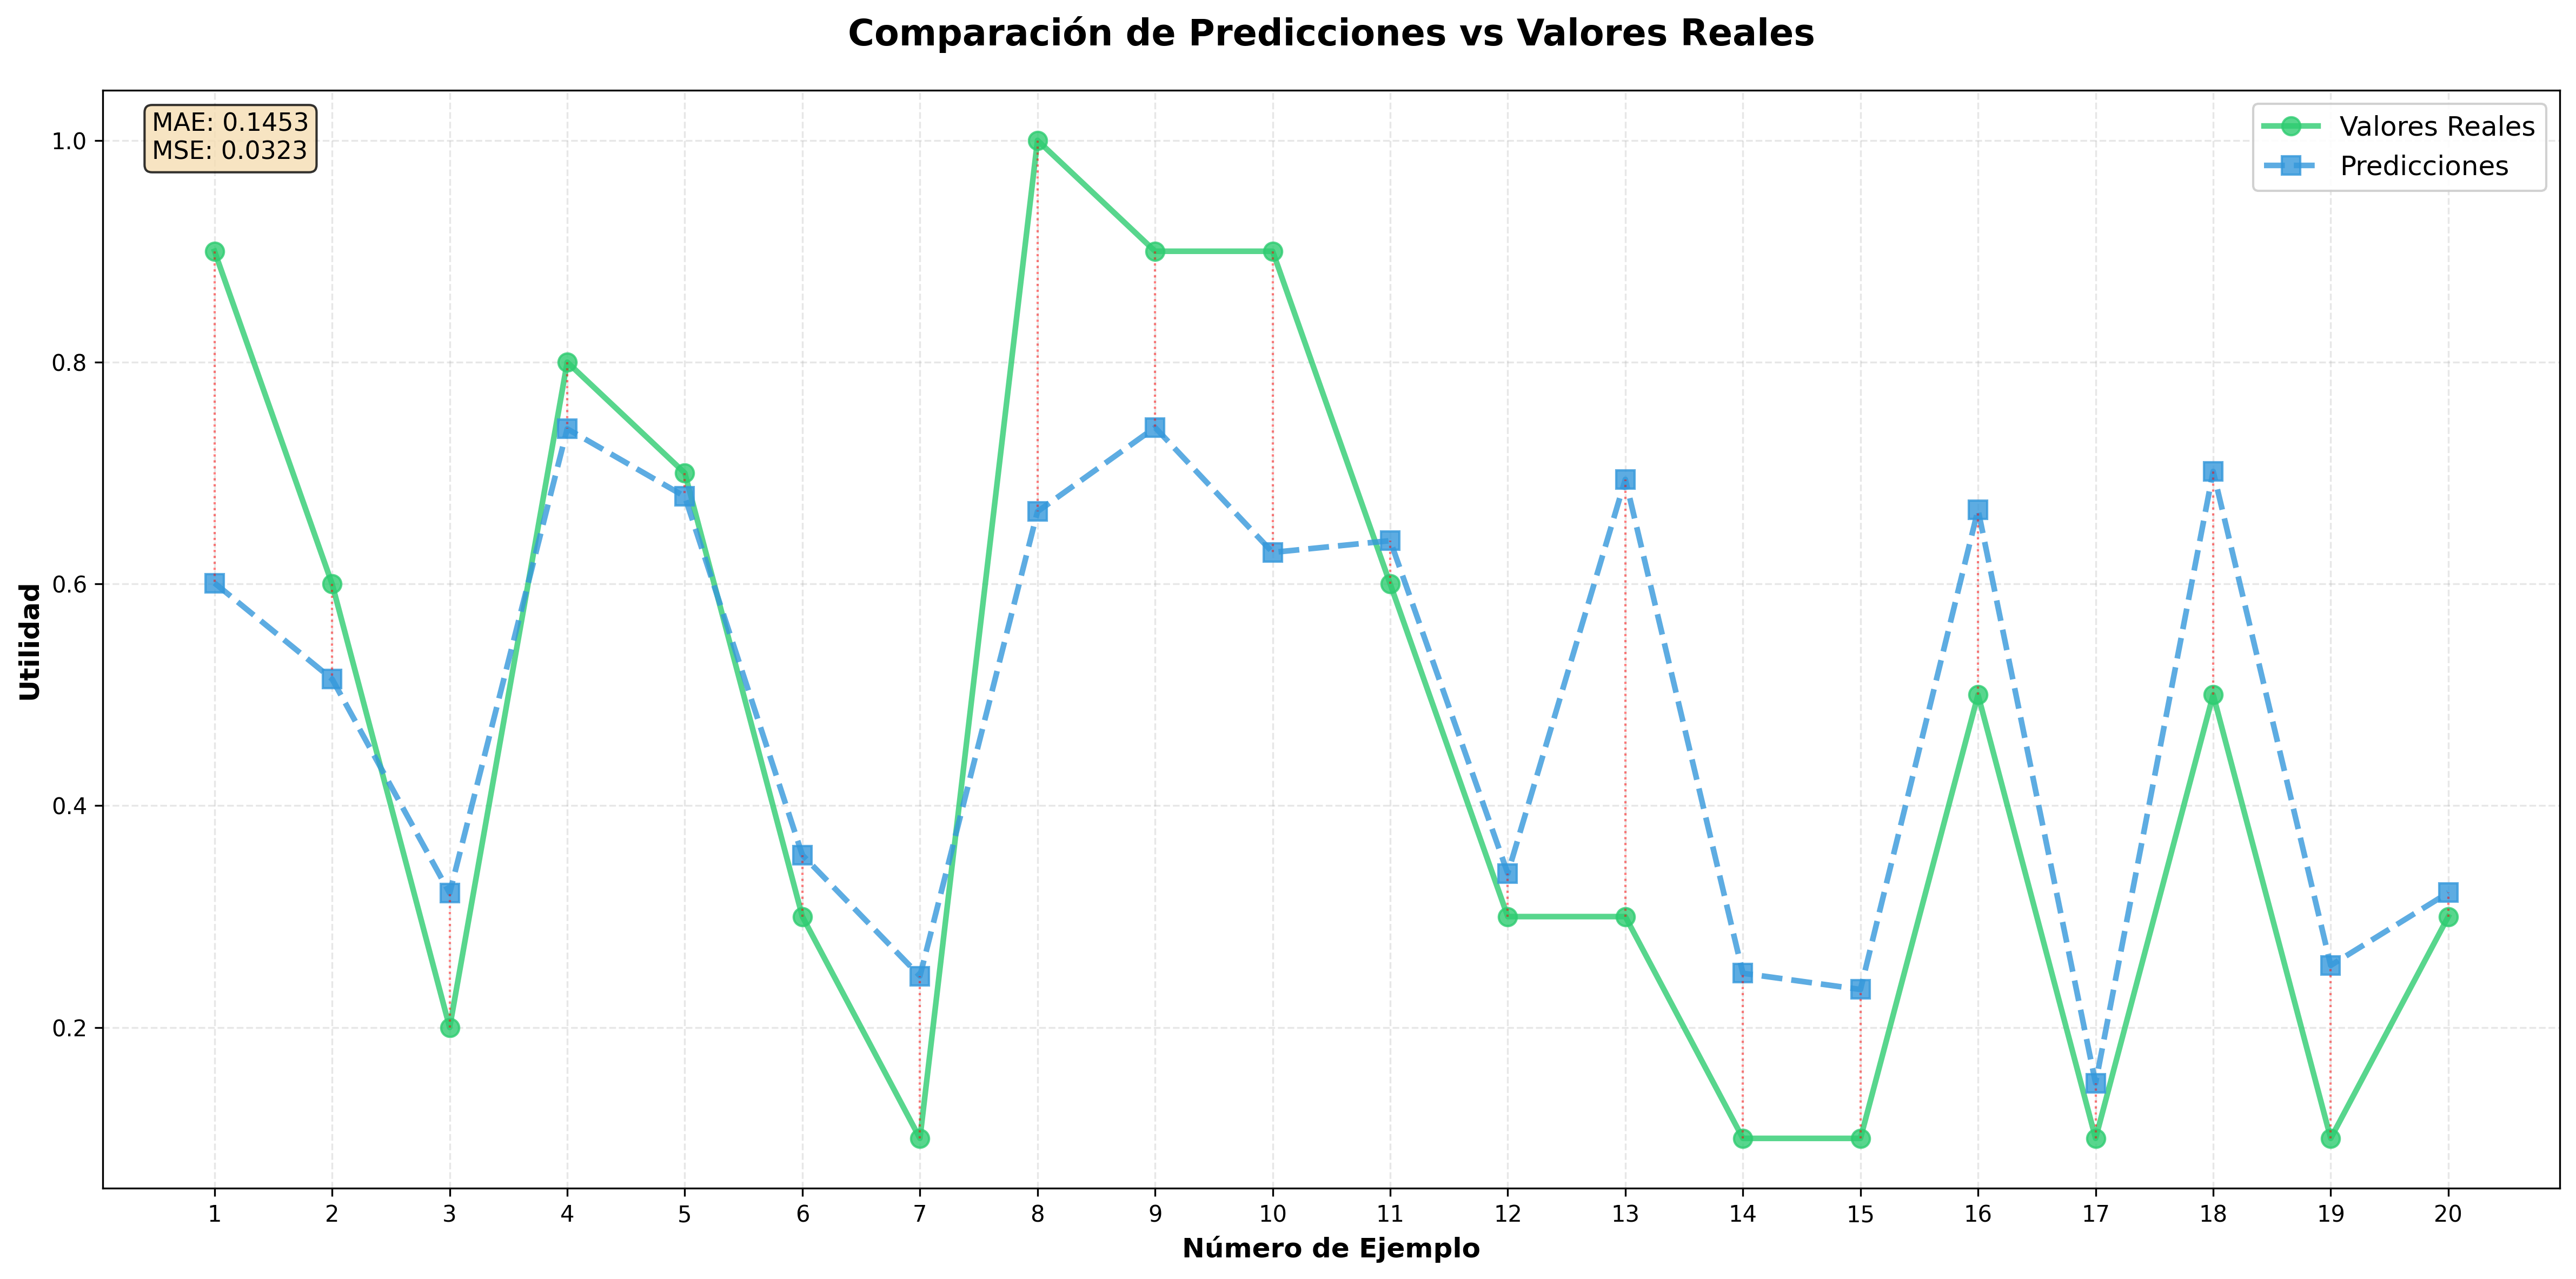
\includegraphics[width=\textwidth]{imaxes/BrazoRobot/UM_prediction_example_100_inverso.png}
  \caption{Predicciones del modelo de utilidad inverso.}
  \label{fig:UM_predicciones_100_inverso}
\end{figure}

Por otra parte, en la figura \ref{fig:UM_training_history_100_inverso} se muestra la evolución del entrenamiento del modelo. Se puede apreciar como tanto el error cuadrático medio y el error 
absoluto medio disminuyen de manera progresiva y se estabilizan tras las primeras etapas. Esto muestra que, además de reducir el error durante el entrenamiento, el modelo también se mantiene 
estable durante la validación.

\begin{figure}[hp!]
  \centering
  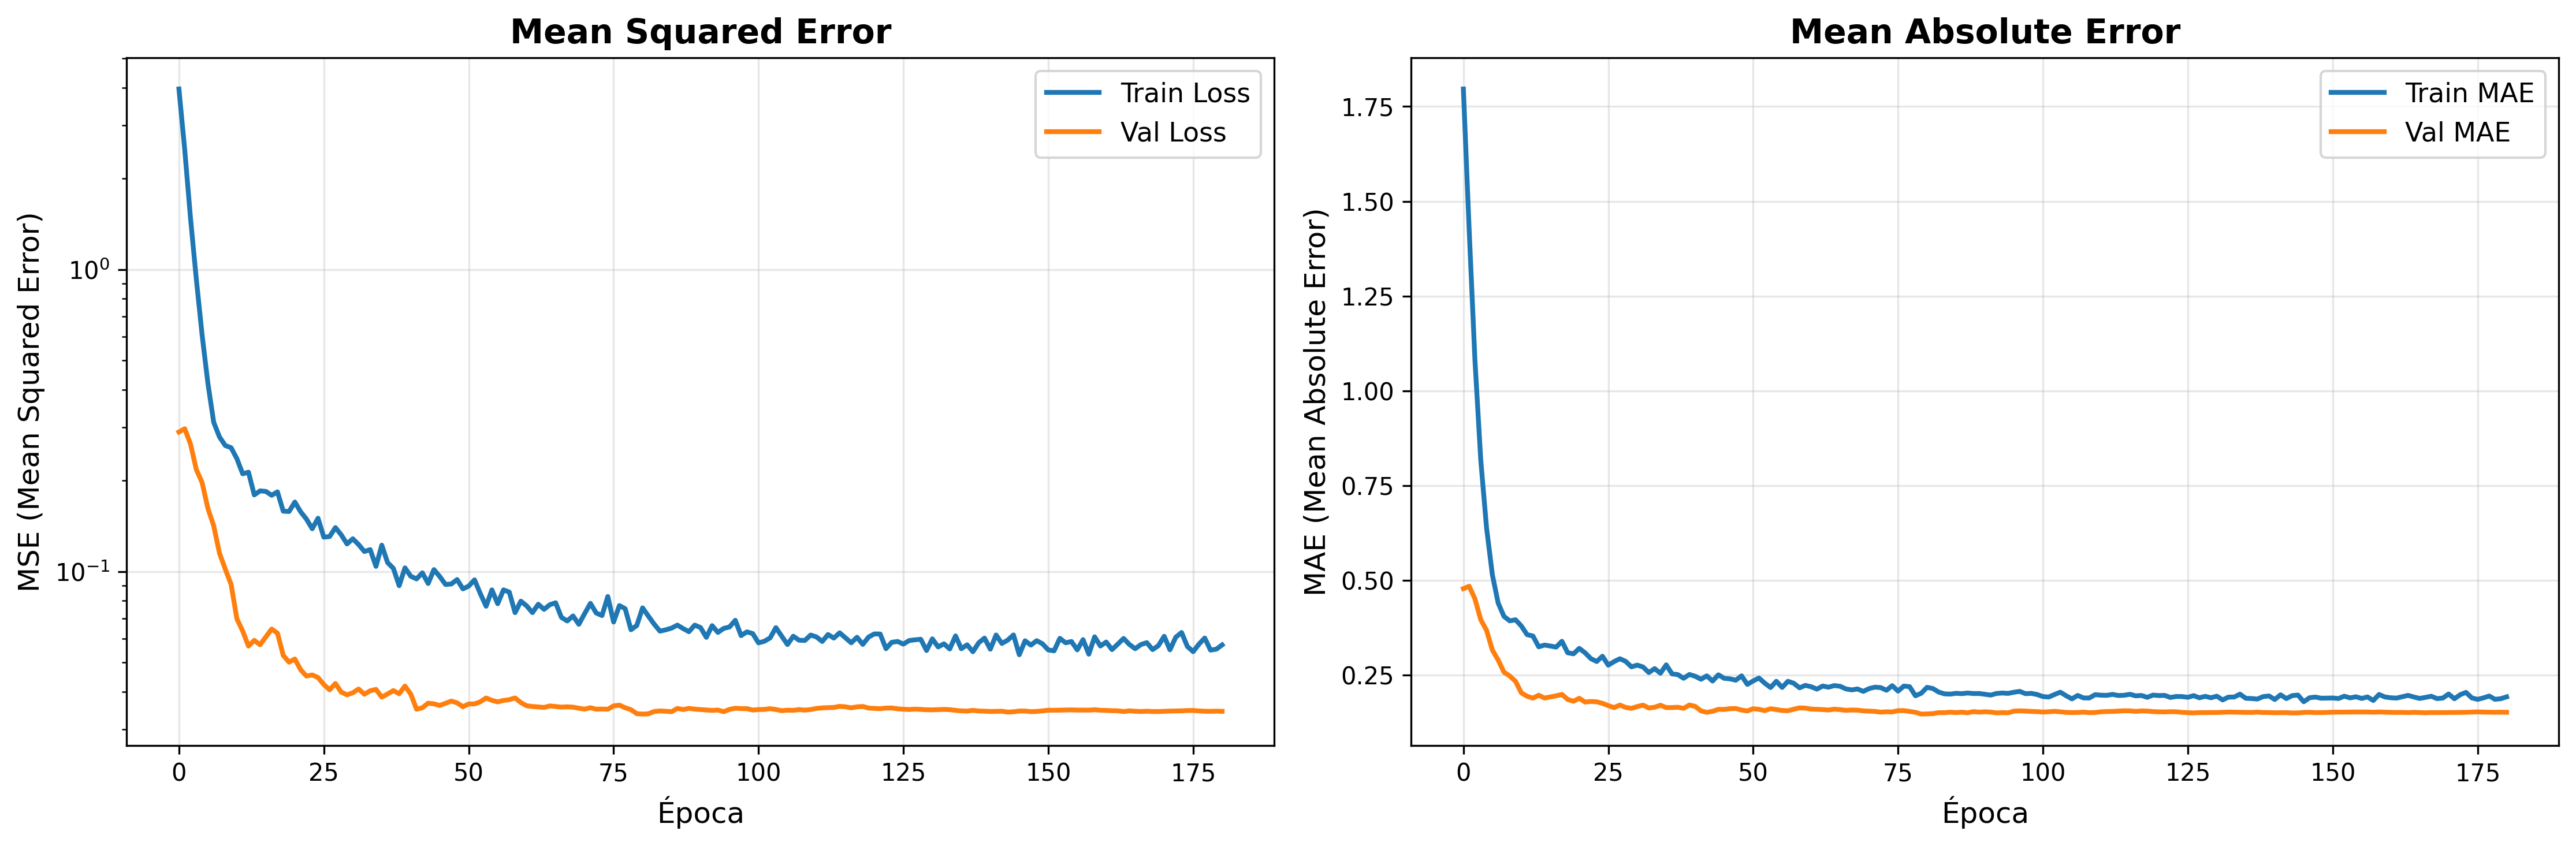
\includegraphics[width=\textwidth]{imaxes/BrazoRobot/UM_training_history_100_inverso.png}
  \caption{Historial de entrenamiento del modelo de utilidad inverso.}
  \label{fig:UM_training_history_100_inverso}
\end{figure}

Para finalizar, al integrar este nuevo modelo de utilidad con el modelo de mundo original, el sistema es capaz de cumplir objetivo, seleccionando acciones que lo llevan a alejarse del objetivo. 
Esto puede apreciarse en la figura \ref{fig:Secuencia_ejecucion_inverso}, que muestra una secuencia de imágenes en la que el robot, que comienza pegado al objetivo, consigue alejarse de él y 
salir del espacio de trabajo.

\begin{figure}[hp!]
  \centering

  \begin{subfigure}[c]{0.45\textwidth}
    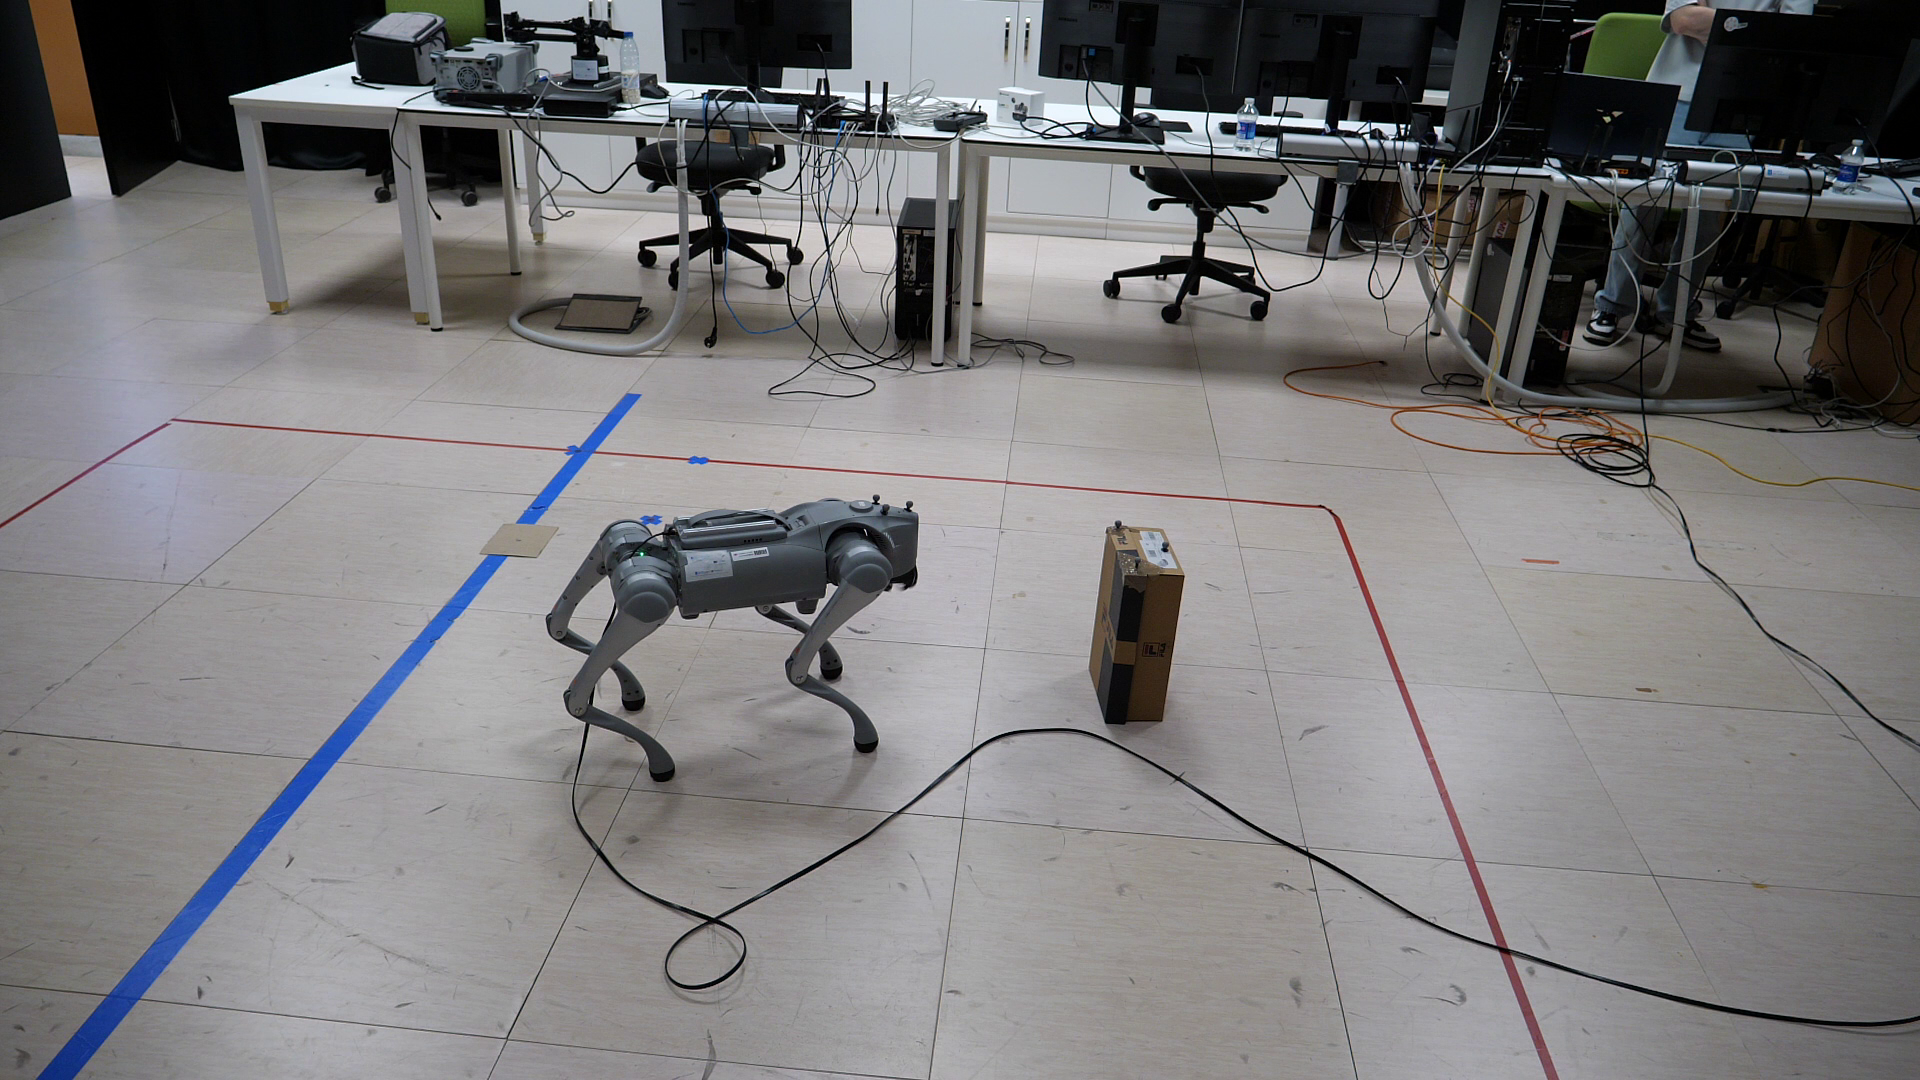
\includegraphics[width=\textwidth]{imaxes/CapturasVideo2/Captura2.1.png}
    \caption{Captura 1.}
    \label{fig:Secuencia_ejecucion_inverso_1}
  \end{subfigure}
  \hfill
  \begin{subfigure}[c]{0.45\textwidth}
    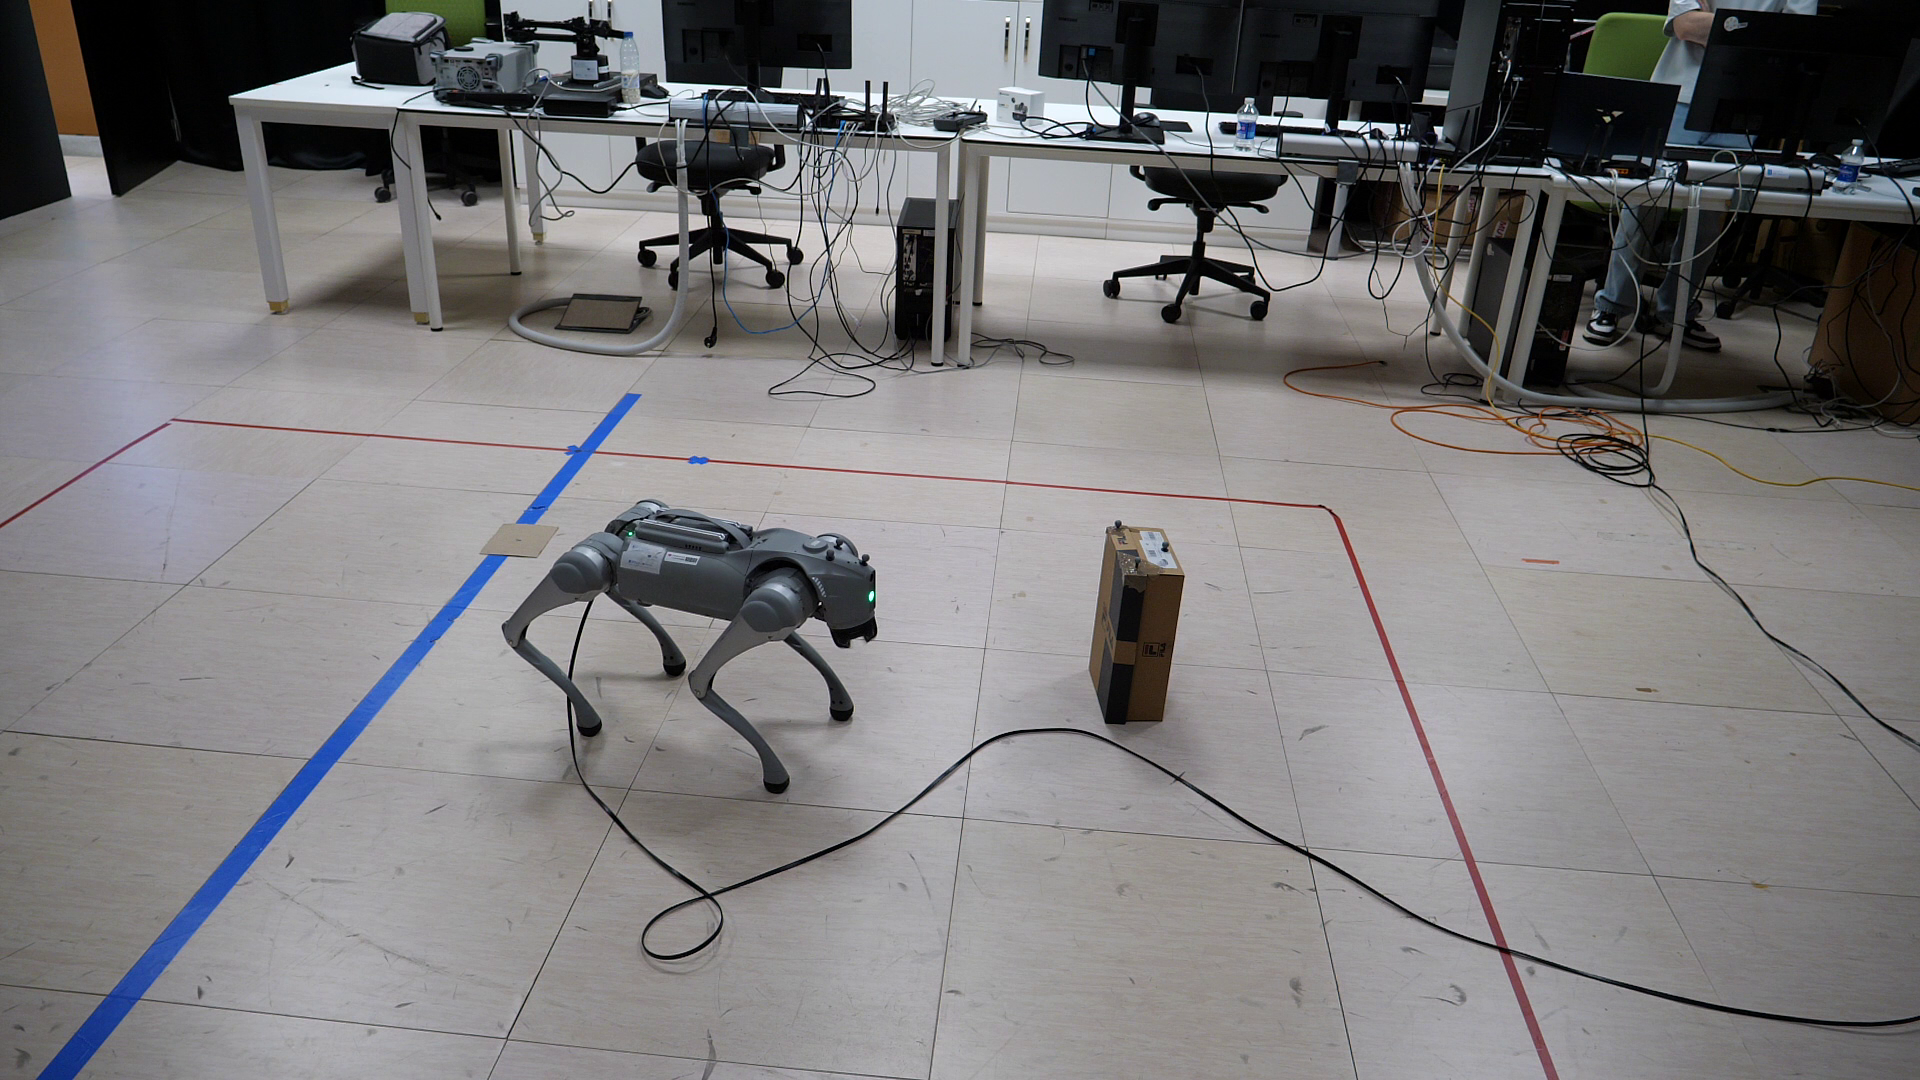
\includegraphics[width=\textwidth]{imaxes/CapturasVideo2/Captura2.2.png}
    \caption{Captura 2.}
    \label{fig:Secuencia_ejecucion_inverso_2}
  \end{subfigure}

  \vspace{0.4cm}

  \begin{subfigure}[c]{0.45\textwidth}
    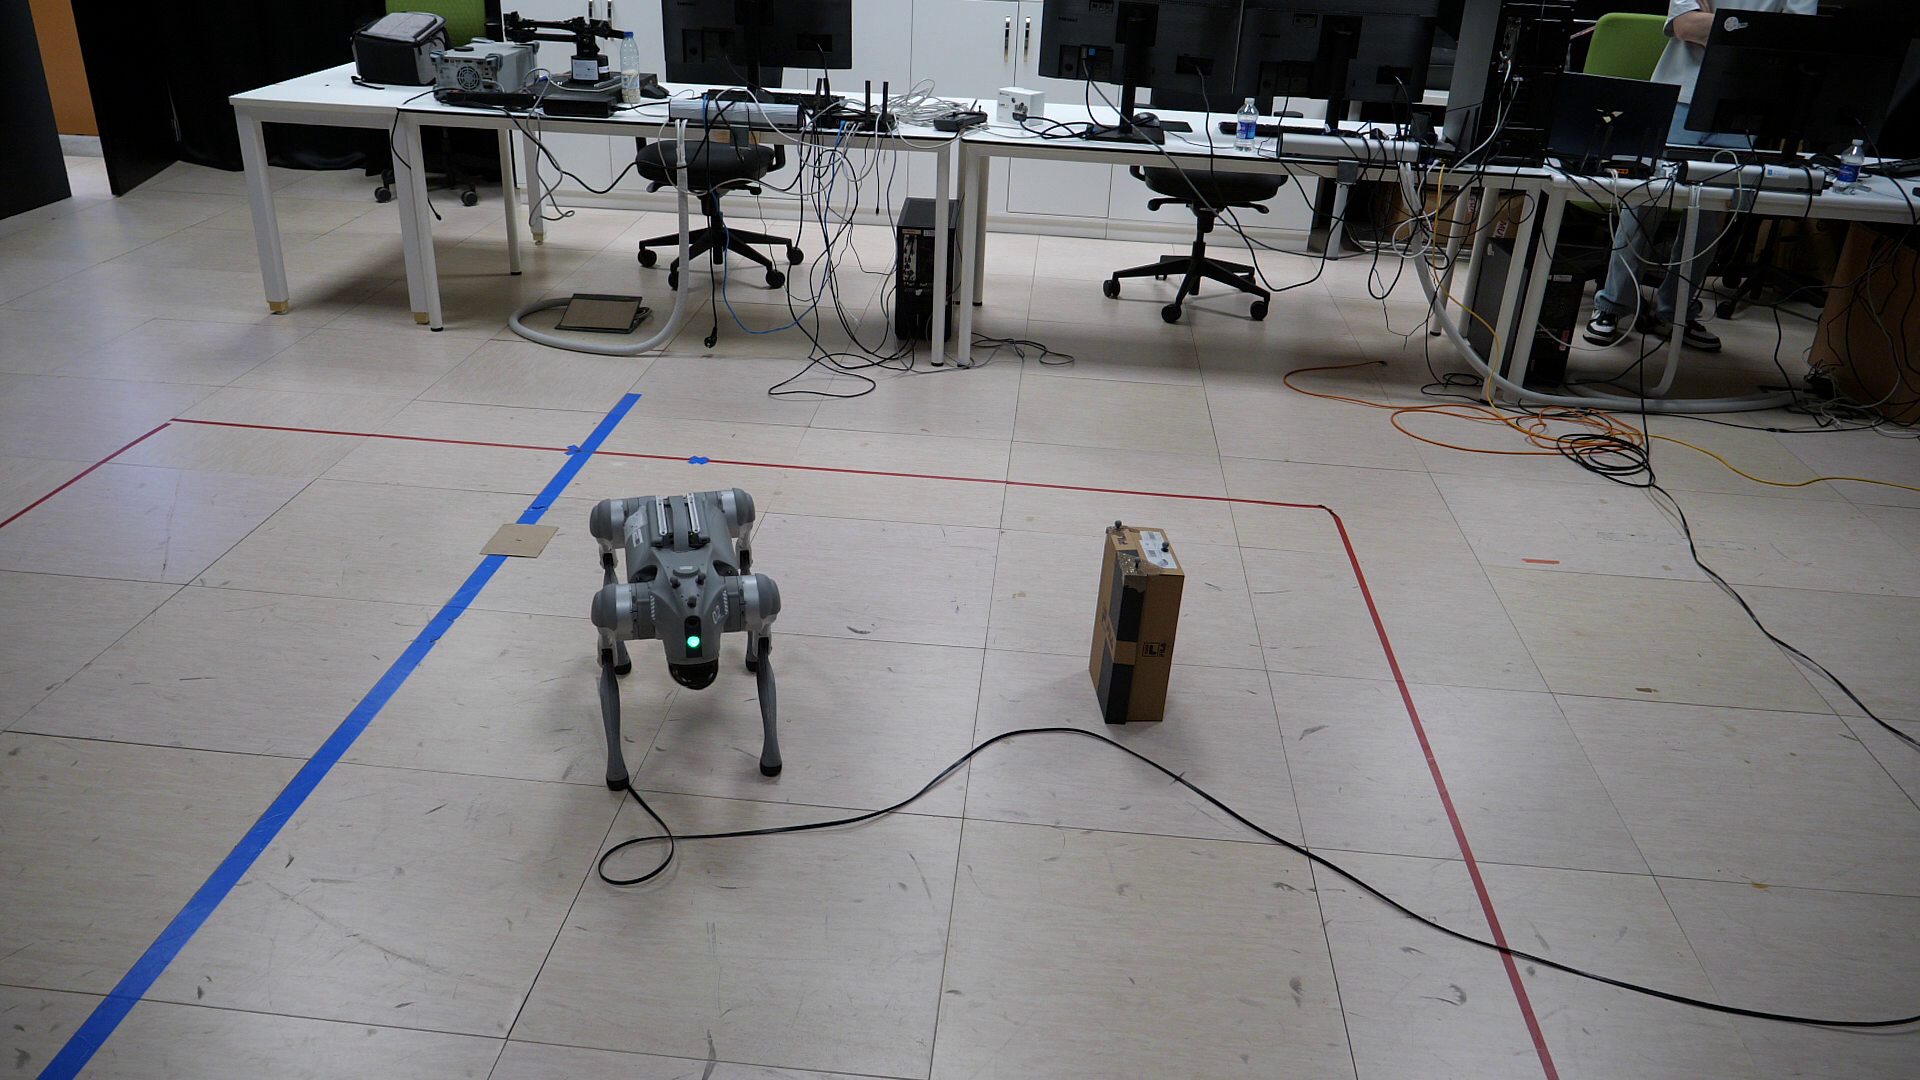
\includegraphics[width=\textwidth]{imaxes/CapturasVideo2/Captura2.3.png}
    \caption{Captura 3.}
    \label{fig:Secuencia_ejecucion_inverso_3}
  \end{subfigure}
  \hfill
  \begin{subfigure}[c]{0.45\textwidth}
    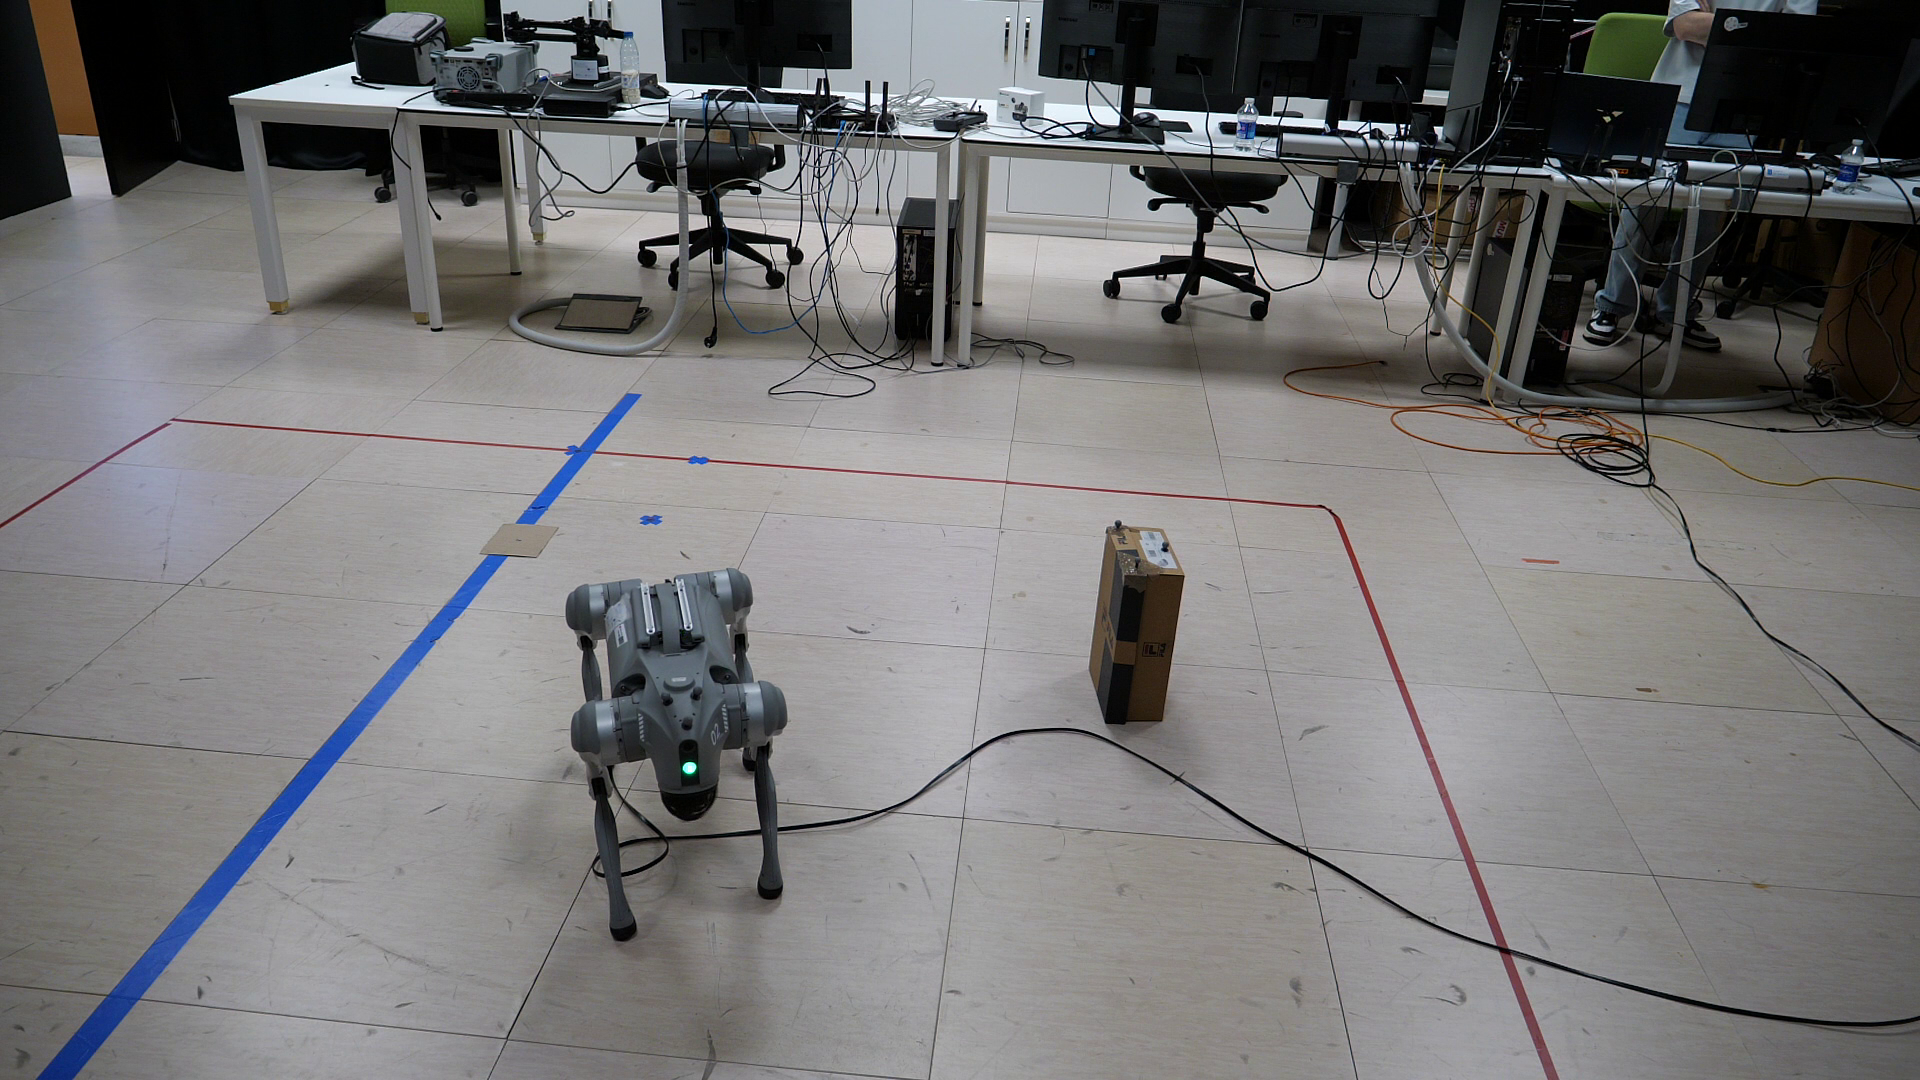
\includegraphics[width=\textwidth]{imaxes/CapturasVideo2/Captura2.4.png}
    \caption{Captura 4.}
    \label{fig:Secuencia_ejecucion_inverso_4}
  \end{subfigure}

  \vspace{0.4cm}

  \begin{subfigure}[c]{0.45\textwidth}
    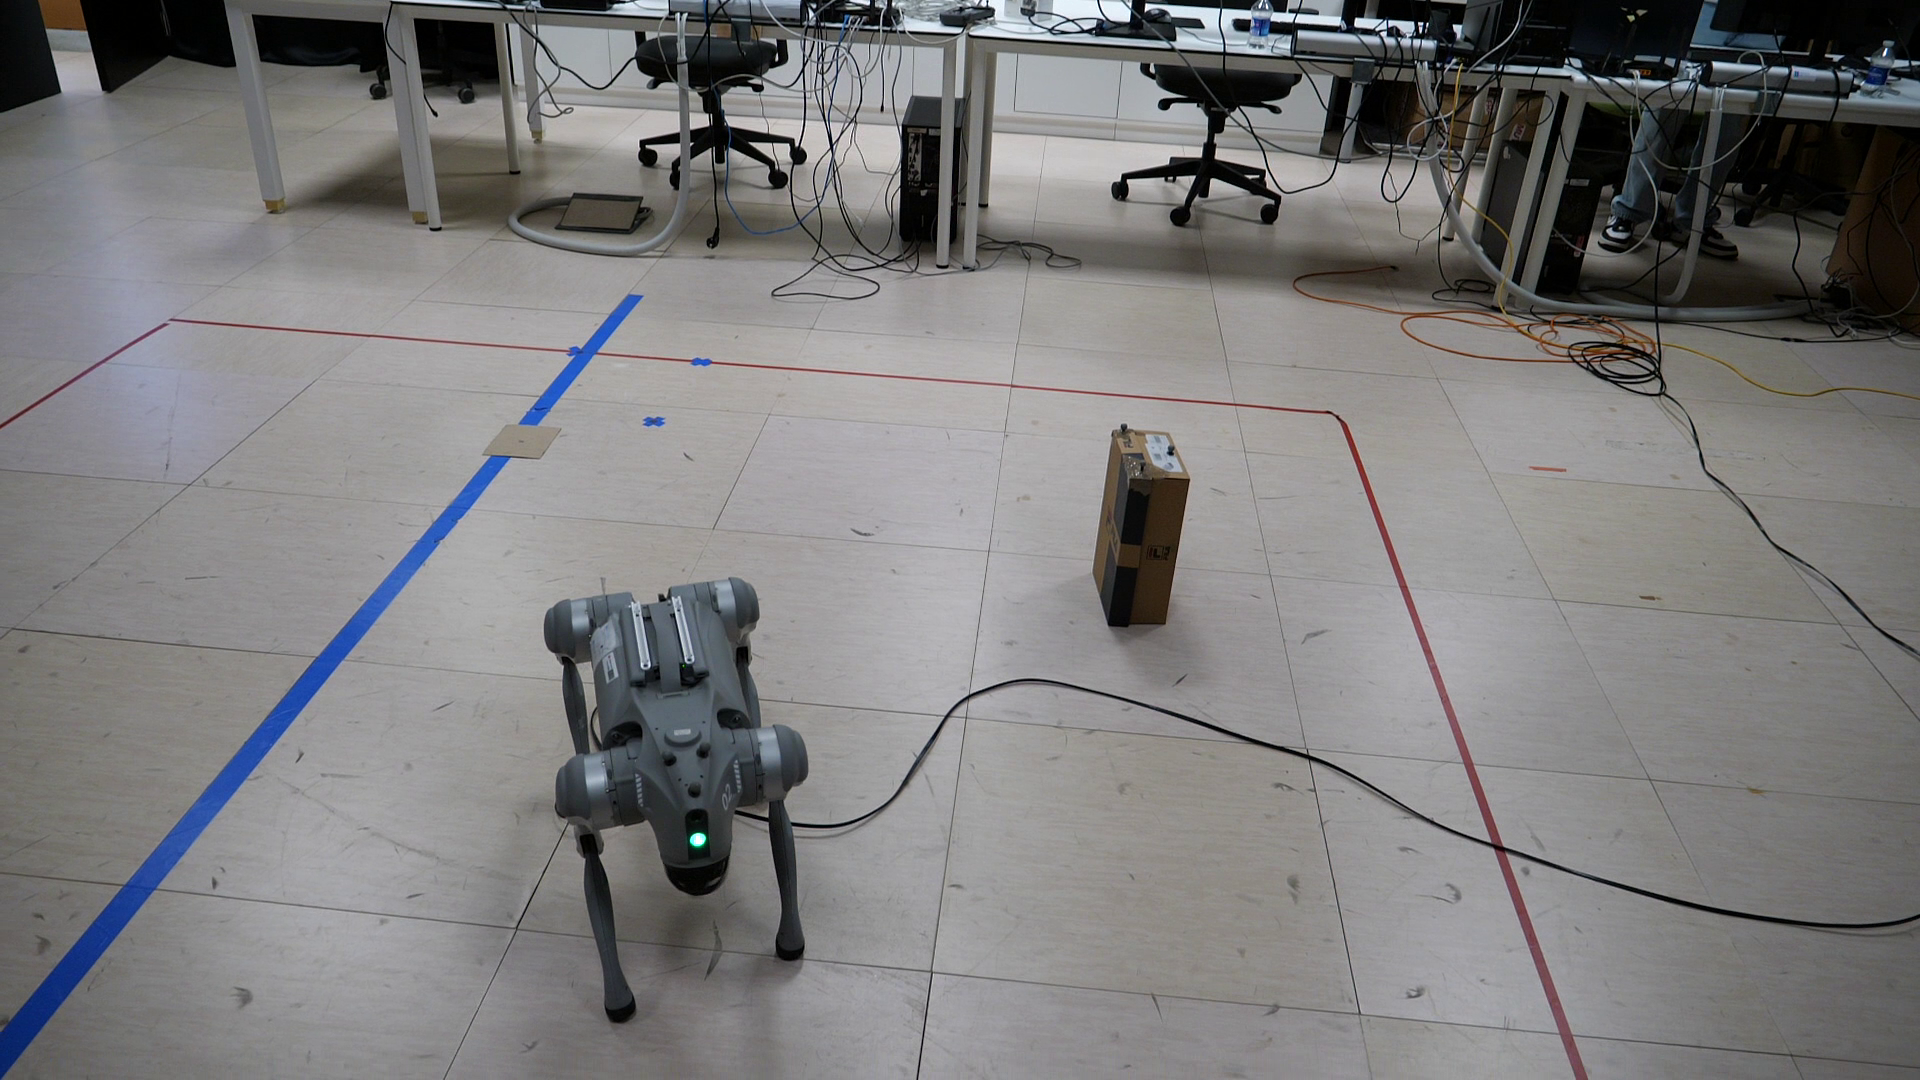
\includegraphics[width=\textwidth]{imaxes/CapturasVideo2/Captura2.5.png}
    \caption{Captura 5.}
    \label{fig:Secuencia_ejecucion_inverso_5}
  \end{subfigure}
  \hfill
  \begin{subfigure}[c]{0.45\textwidth}
    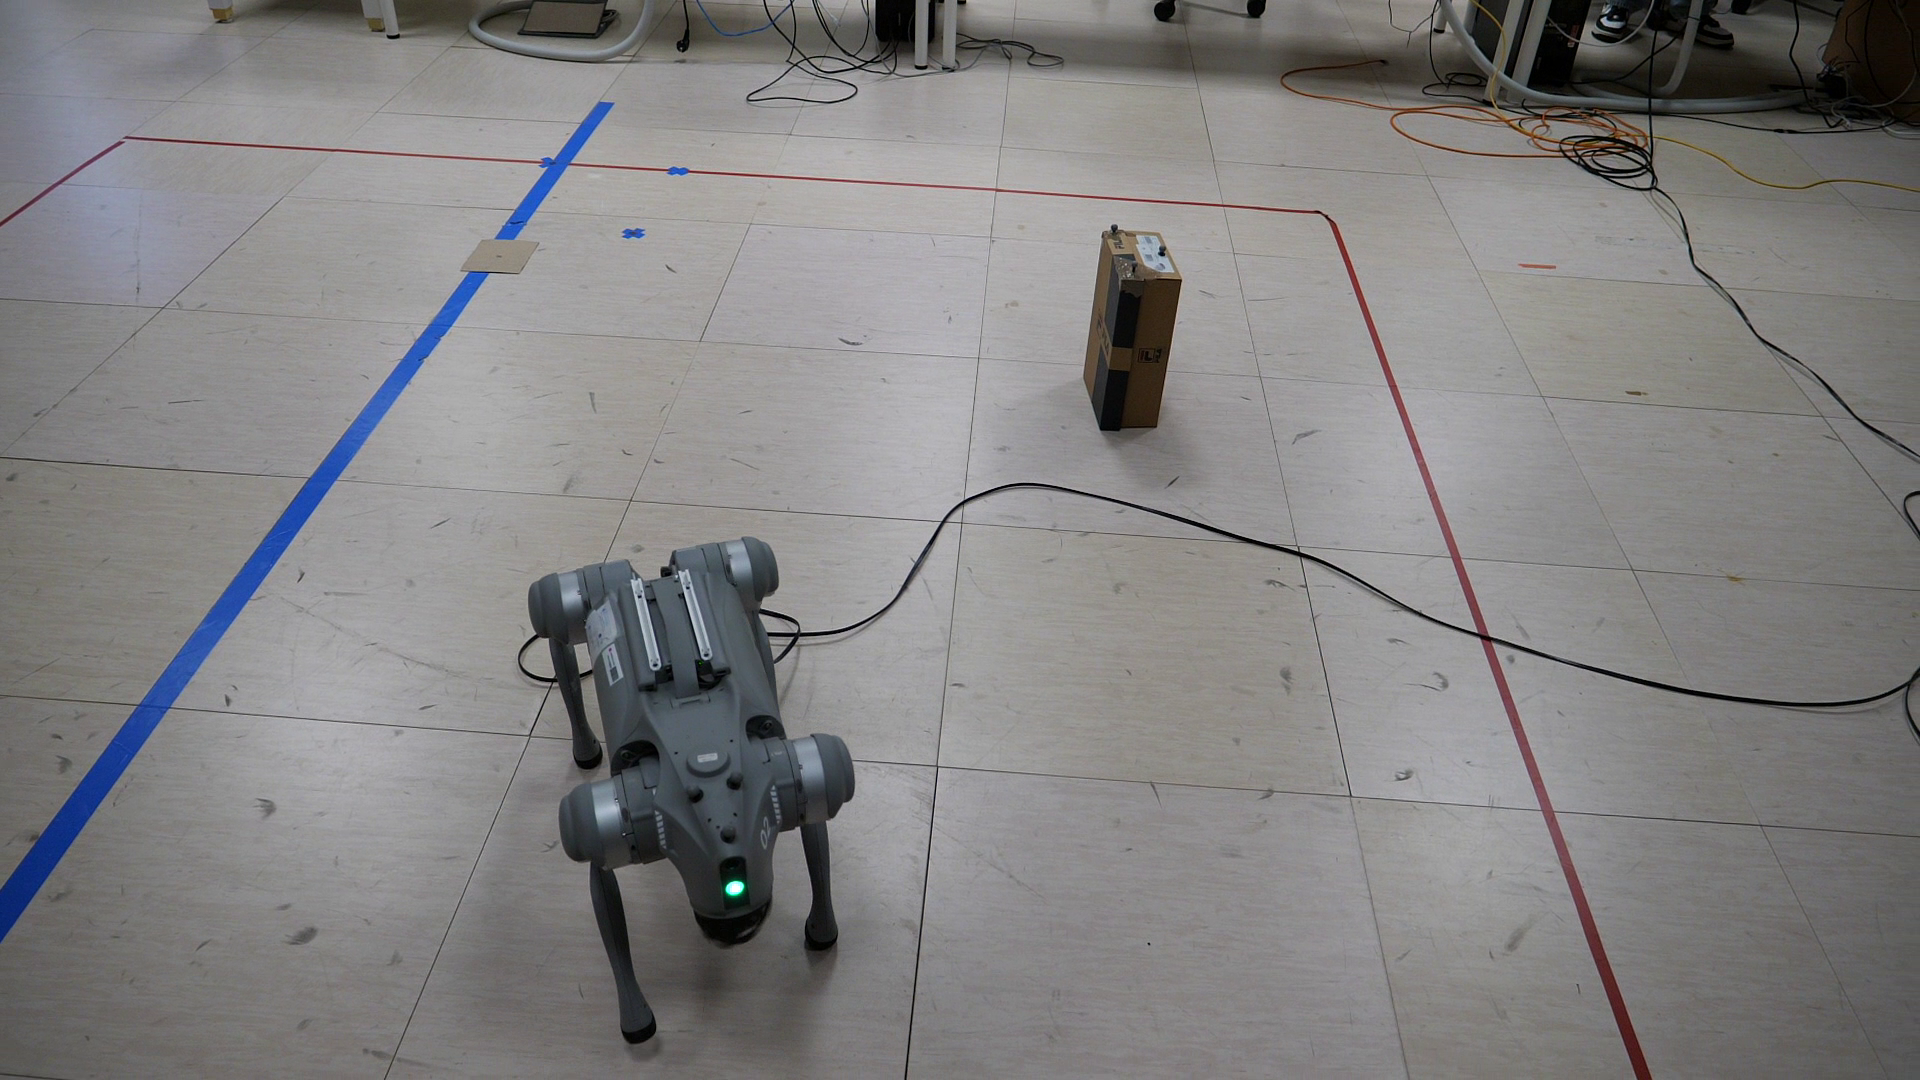
\includegraphics[width=\textwidth]{imaxes/CapturasVideo2/Captura2.6.png}
    \caption{Captura 6.}
    \label{fig:Secuencia_ejecucion_inverso_6}
  \end{subfigure}

  \vspace{0.4cm}

  \begin{subfigure}[c]{0.45\textwidth}
    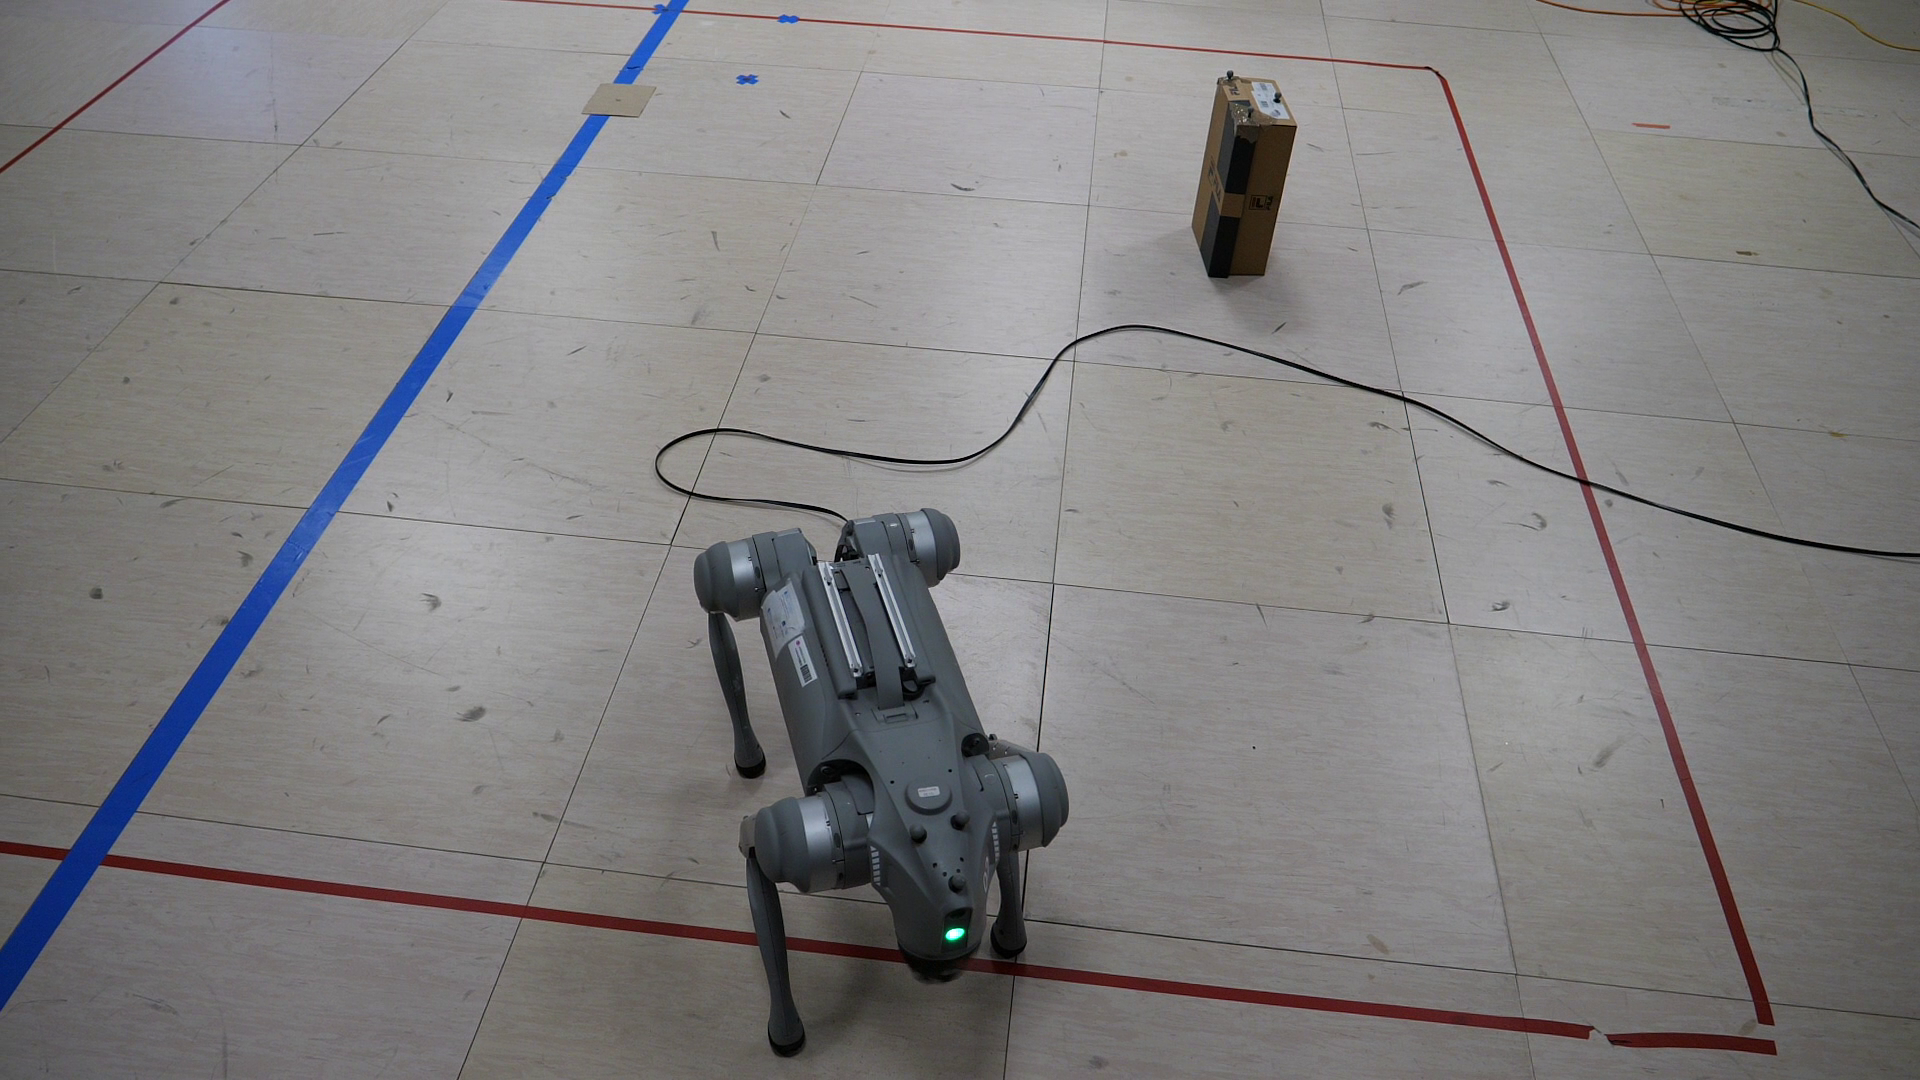
\includegraphics[width=\textwidth]{imaxes/CapturasVideo2/Captura2.7.png}
    \caption{Captura 7.}
    \label{fig:Secuencia_ejecucion_inverso_7}
  \end{subfigure}
  \hfill

  \caption{Secuencia de imagenes de una ejecución con el modelo de utilidad nuevo.}
  \label{fig:Secuencia_ejecucion_inverso}
\end{figure}

En la figura \ref{fig:grafica_relacion_ut_dist_inverso} se observa la relación entre la distancia con el objetivo y los valores de utilidad para cada una de las iteraciones que componen la 
ejecución. Se puede apreciar como en este caso los valores de ambos convergen a medida que el robot se aleja del objetivo, a diferencia que el caso del modelo original que se separaban. Este 
comportamiento es el esperado para esta meta y confirma que el modelo ha sido capaz de aprender la relación entre las observaciones y la utilidad de estas para conseguir alejarse del objetivo.

\begin{figure}[hp!]
  \centering
  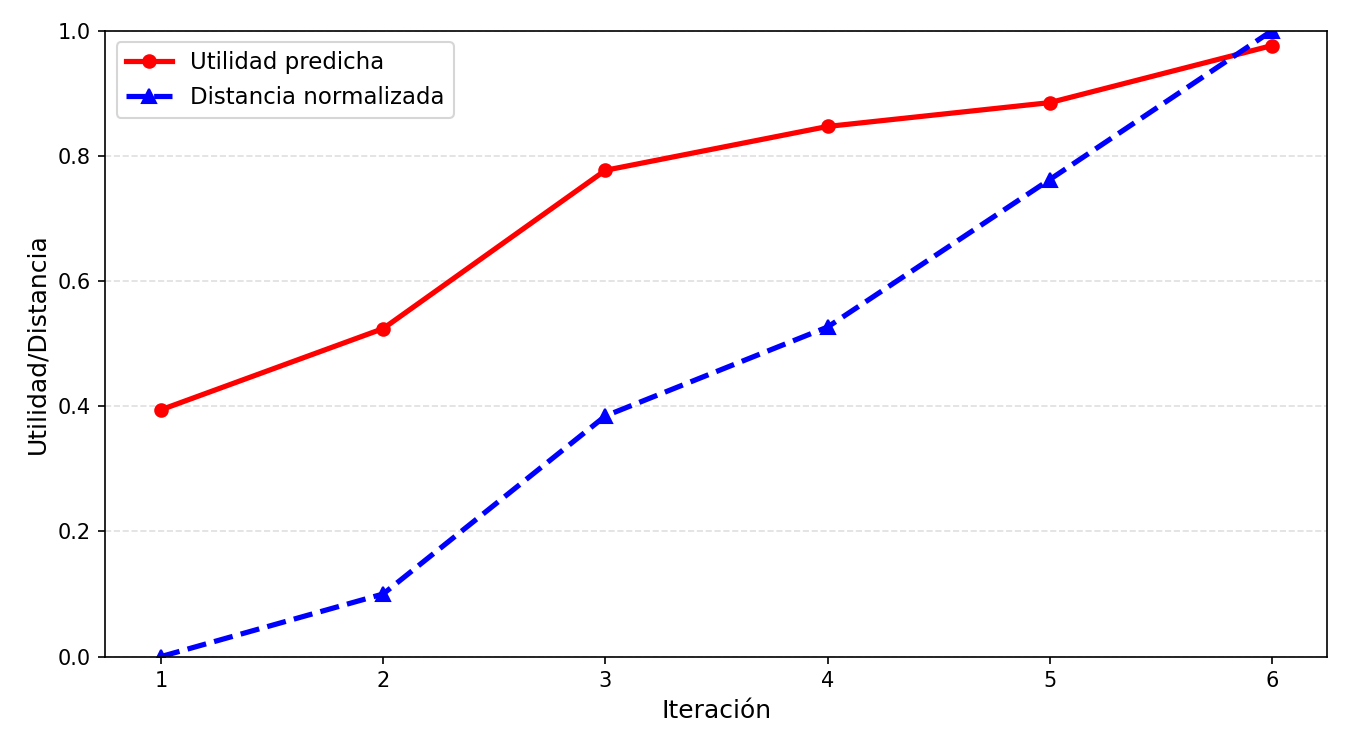
\includegraphics[width=0.75\textwidth]{imaxes/BrazoRobot/grafica_relacion_ut_dist_inverso.png}
  \caption{Gráfica de la relación entre la utilidad y la distancia para cada iteración con el modelo de utilidad nuevo.}
  \label{fig:grafica_relacion_ut_dist_inverso}
\end{figure}

De esta manera se demuestra que el modelo de mundo pudo reutilizarse sin necesidad de volver a entrenarlo, ya que las predicciones proporcionadas por este siguen siendo válidas para en 
este entorno. De esta manera, se confirma que una misma dinámica del entorno puede ser utilizada para resolver distintas metas.


\subsubsection{Diferente modelo de mundo, mismo modelo de utilidad}

En segundo lugar, se comprobó si el modelo de utilidad original se podía emplear con un modelo de mundo diferente. Para esto, se desarrolló una simulación sencilla de un brazo robótico en 
2D (como se puede apreciar en la figura \ref{fig:esq_brazo_robot}), formado por dos segmentos unidos con origen en el punto (0, 0). El objetivo de esta prueba era comprobar si el modelo de 
utilidad podía seguir utilizándose en otro sistema, siempre y cuando, las observaciones generadas por el nuevo modelo de mundo mantuviese una estructura compatible.

\begin{figure}[hp!]
  \centering
  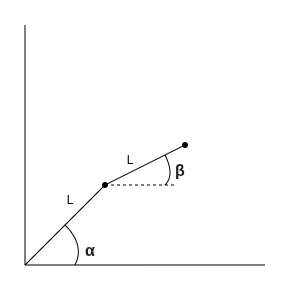
\includegraphics[width=0.5\textwidth]{imaxes/EsquemaBrazoRobot.png}
  \caption{Esquema del brazo robótico.}
  \label{fig:esq_brazo_robot}
\end{figure}

Para calcular la posición de este brazo robótico se utilizaron las siguientes fórmulas:

Para calcular el punto (\(x_1, y_1\)) correspondiente al primer segmento se utiliza la fórmula:

\[
x_1 = L \cdot \cos(\alpha)
\]
  
\[
y_1 = L \cdot \sin(\alpha)
\]

y para el punto final (\(x_2, y_2\)) del segundo segmento se emplea:

\[
x_2 = x_1 + L \cdot \cos(\alpha)
\]
  
\[
y_2 = y_1 + L \cdot \sin(\alpha)
\]

Al sustituir \(x_1\) e \(y_1\) en la segunda operación, se calcula directamente el punto final. La fórmula resultante es la siguiente:

\[
x_2 = L \cdot (\cos(\alpha) + \cos(\beta))
\]

\[
y_2 = L \cdot (\sin(\alpha) + \sin(\beta))
\]

De esta manera, mediante esta fórmula, se calcula la posición del punto final del brazo (\(x_2, y_2\)) en función de la longitud de los segmentos (L) y dos ángulos (\(\alpha\) y \(\beta\)). Este 
punto final debía acercarse a otro punto objetivo, generado previamente dentro del espacio que el brazo podía alcanzar.

El nuevo modelo de mundo no representa el movimiento del robot Go2, sino que describe la evolución del extremo del brazo robótico al modificar los ángulos que forman sus articulaciones. A 
partir de las acciones definidas, las cuales son incrementos y decrementos de los ángulos (\(\alpha\) y \(\beta\)), el modelo debía predecir el nuevo estado del brazo. Este estado fue necesario 
expresarlo de forma compatible con el modelo de utilidad, permitiendo que éste evalúe si la posición resultante de la acción era conveniente para acercarse al objetivo.

En referente a este último punto, fue necesario adaptar manualmente las observaciones para hacerlas compatibles con el modelo de utilidad original. Las observaciones originales estaban formadas 
por la tupla de distancia, ángulo respecto al objetivo y ángulo sobre sí mismo, sin embargo las observaciones que se obtienen del brazo robótico son solamente la distancia y el ángulo respecto 
al objetivo. Si no se adaptasen estas observaciones para hacer compatibles las salidas del modelo de mundo con las entradas del modelo de utilidad el sistema no podría funcionar. Con el fin de 
solventar este problema, se realizó una adaptación a la hora de comunicar las observaciones entre los modelos. El modelo de mundo trabajaría únicamente con distancia y ángulo respecto al 
objetivo, pero a la hora de realizar esta comunicación se añadiría un tercer elemento a la tupla que sustituiría al ángulo respecto a sí mismo. El valor de este elemento se pondría a 0.

En cuanto al proceso de recolección de datos y entrenamiento del modelo se realizó de manera similar al realizado con el modelo original del robot Go2. Para obtener el conjunto de datos de 
entrenamiento se ejecutó una simulación en Python (sin interfaz gráfica) en la que en cada iteración se calculaba la posición del brazo antes y después de realizar la acción mediante la fórmula 
explicada previamente. Estas acciones se definieron como incrementos o decrementos en ambos ángulos, los cuales se seleccionan de manera aleatoria en un intervalo de 15º a -15º. Tras 
aproximadamente 30 minutos de ejecución se recolectaron un total de 8365 muestras.

El siguiente paso era entrenar el modelo de utilidad con los datos recolectados. Para esto se empleó el mismo proceso que con los modelos previos. Se realizó el preprocesado de datos igual 
que en apartados anteriores y se seleccionó una estructura de red de 4 capas con 64, 128, 64 y 32 neuronas respectivamente. Se utilizó Adam como optimizador y el MSE y MAE como métricas. También 
se contó con un Early Stop con 100 épocas de paciencia y una reducción del learning rate.

Los resultados del entrenamiento de este nuevo modelo se muestran en la figura \ref{fig:brazorobot_WM_training_history}. En ella se observa una reducción tanto del MSE como del MAE durante las 
primeras épocas y una estabilización posterior, indicando que el modelo aprendió de manera adecuada la relación entre las acciones y el estado posterior a ellas.

\begin{figure}[hp!]
  \centering
  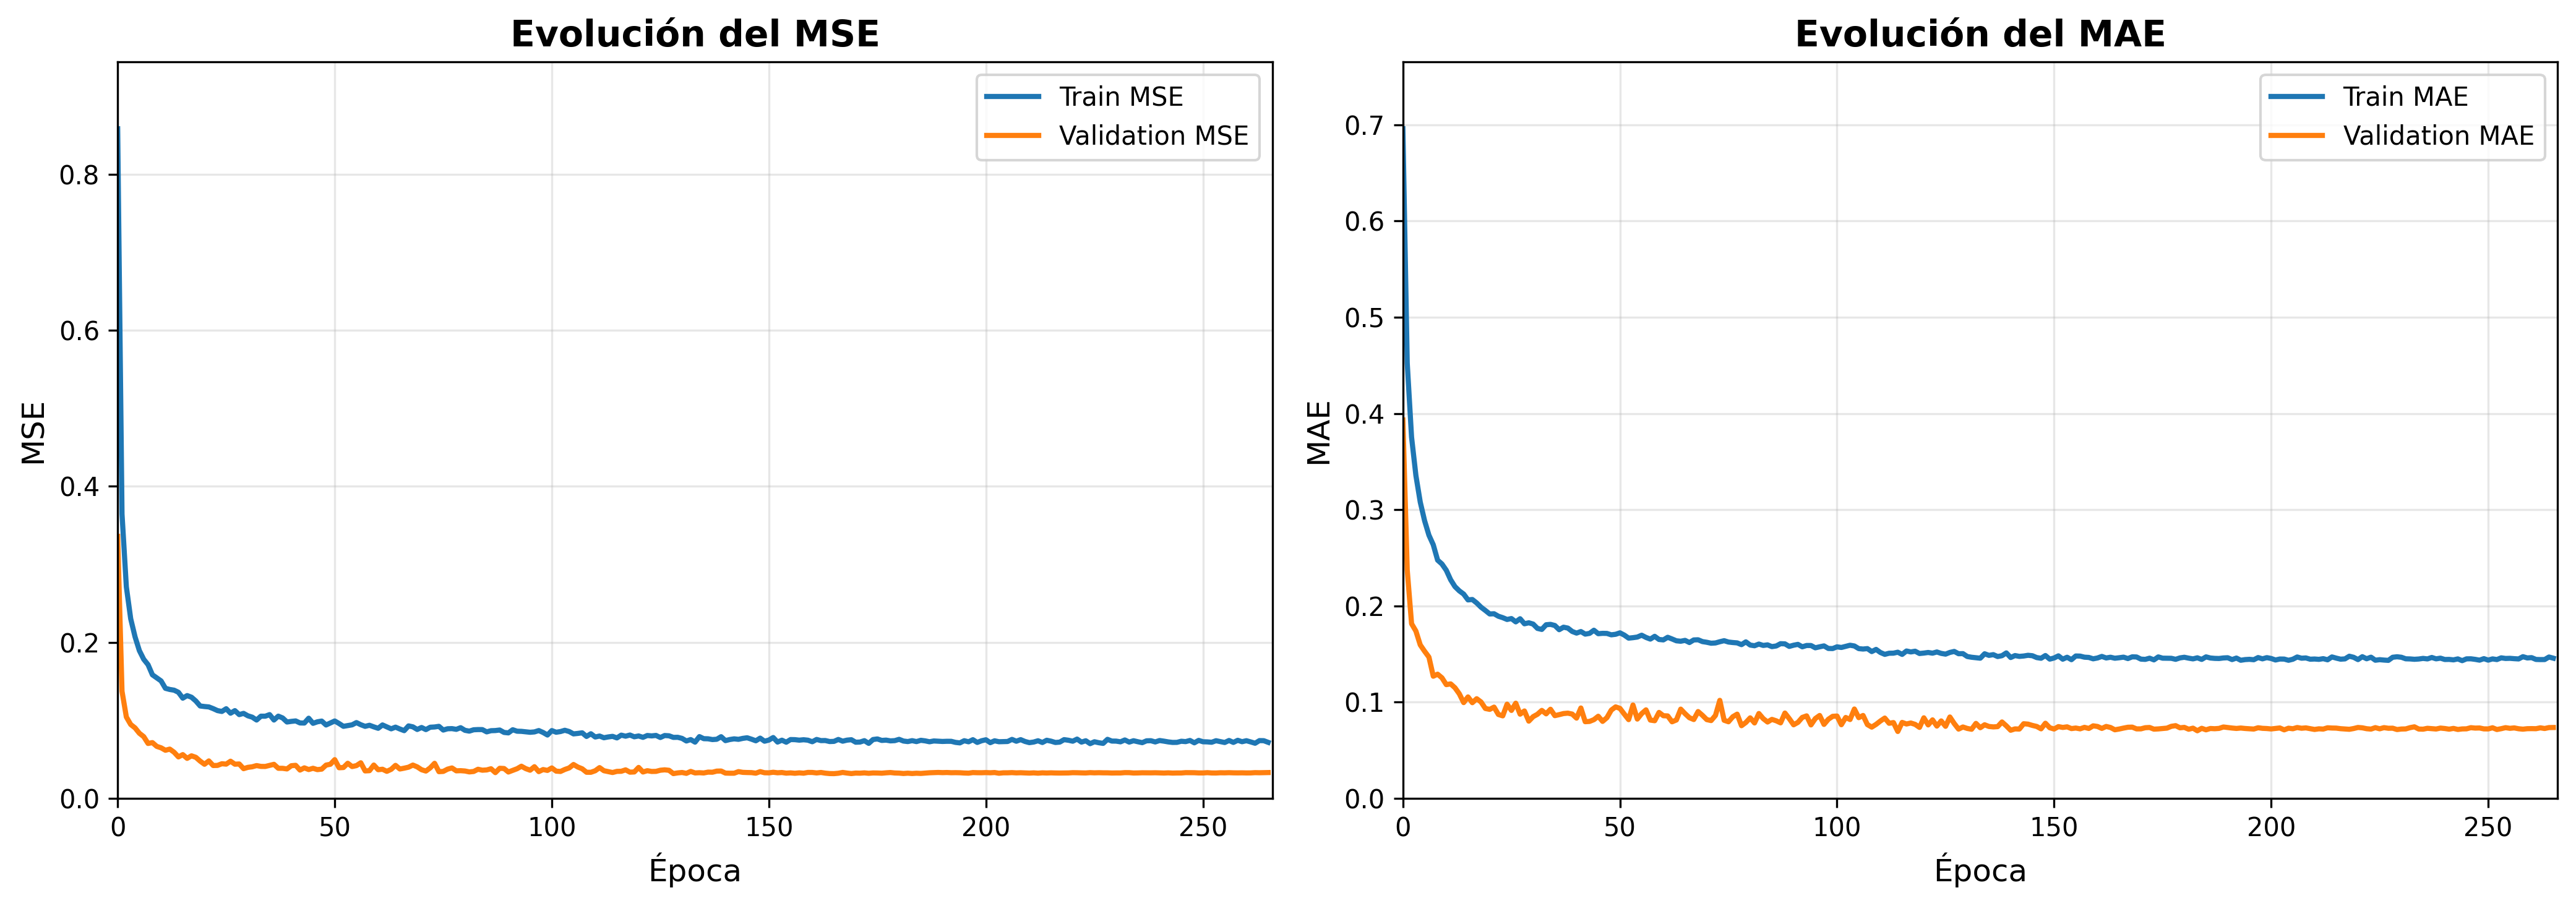
\includegraphics[width=\textwidth]{imaxes/BrazoRobot/WM_Brazo_training_metrics.png}
  \caption{Historial de entrenamiento del modelo de mundo para el brazo robot.}
  \label{fig:brazorobot_WM_training_history}
\end{figure}

La figura \ref{fig:brazorobot_WM_predictions} muestra la comparación entre los valores reales y las predicciones del modelo. En este caso se añadió otra métrica, la \(R^2\) , que indica la 
precisión del modelo a la hora de predecir los valores. En el caso de la distancia, el ajuste es muy preciso, presentando un valor de \(R^2\) de 0.9924. Para el ángulo respecto al objetivo, el 
resultado también se puede considerar satisfactorio pero es menos preciso y comete más errores, pudiendo observar una mayor dispersión en algunos puntos, con un \(R^2\) de 0.9173. Esta diferencia 
se puede considerar razonable, debido a que el ángulo puede variar de forma más sensible ante pequeños cambios.

\begin{figure}[hp!]
  \centering
  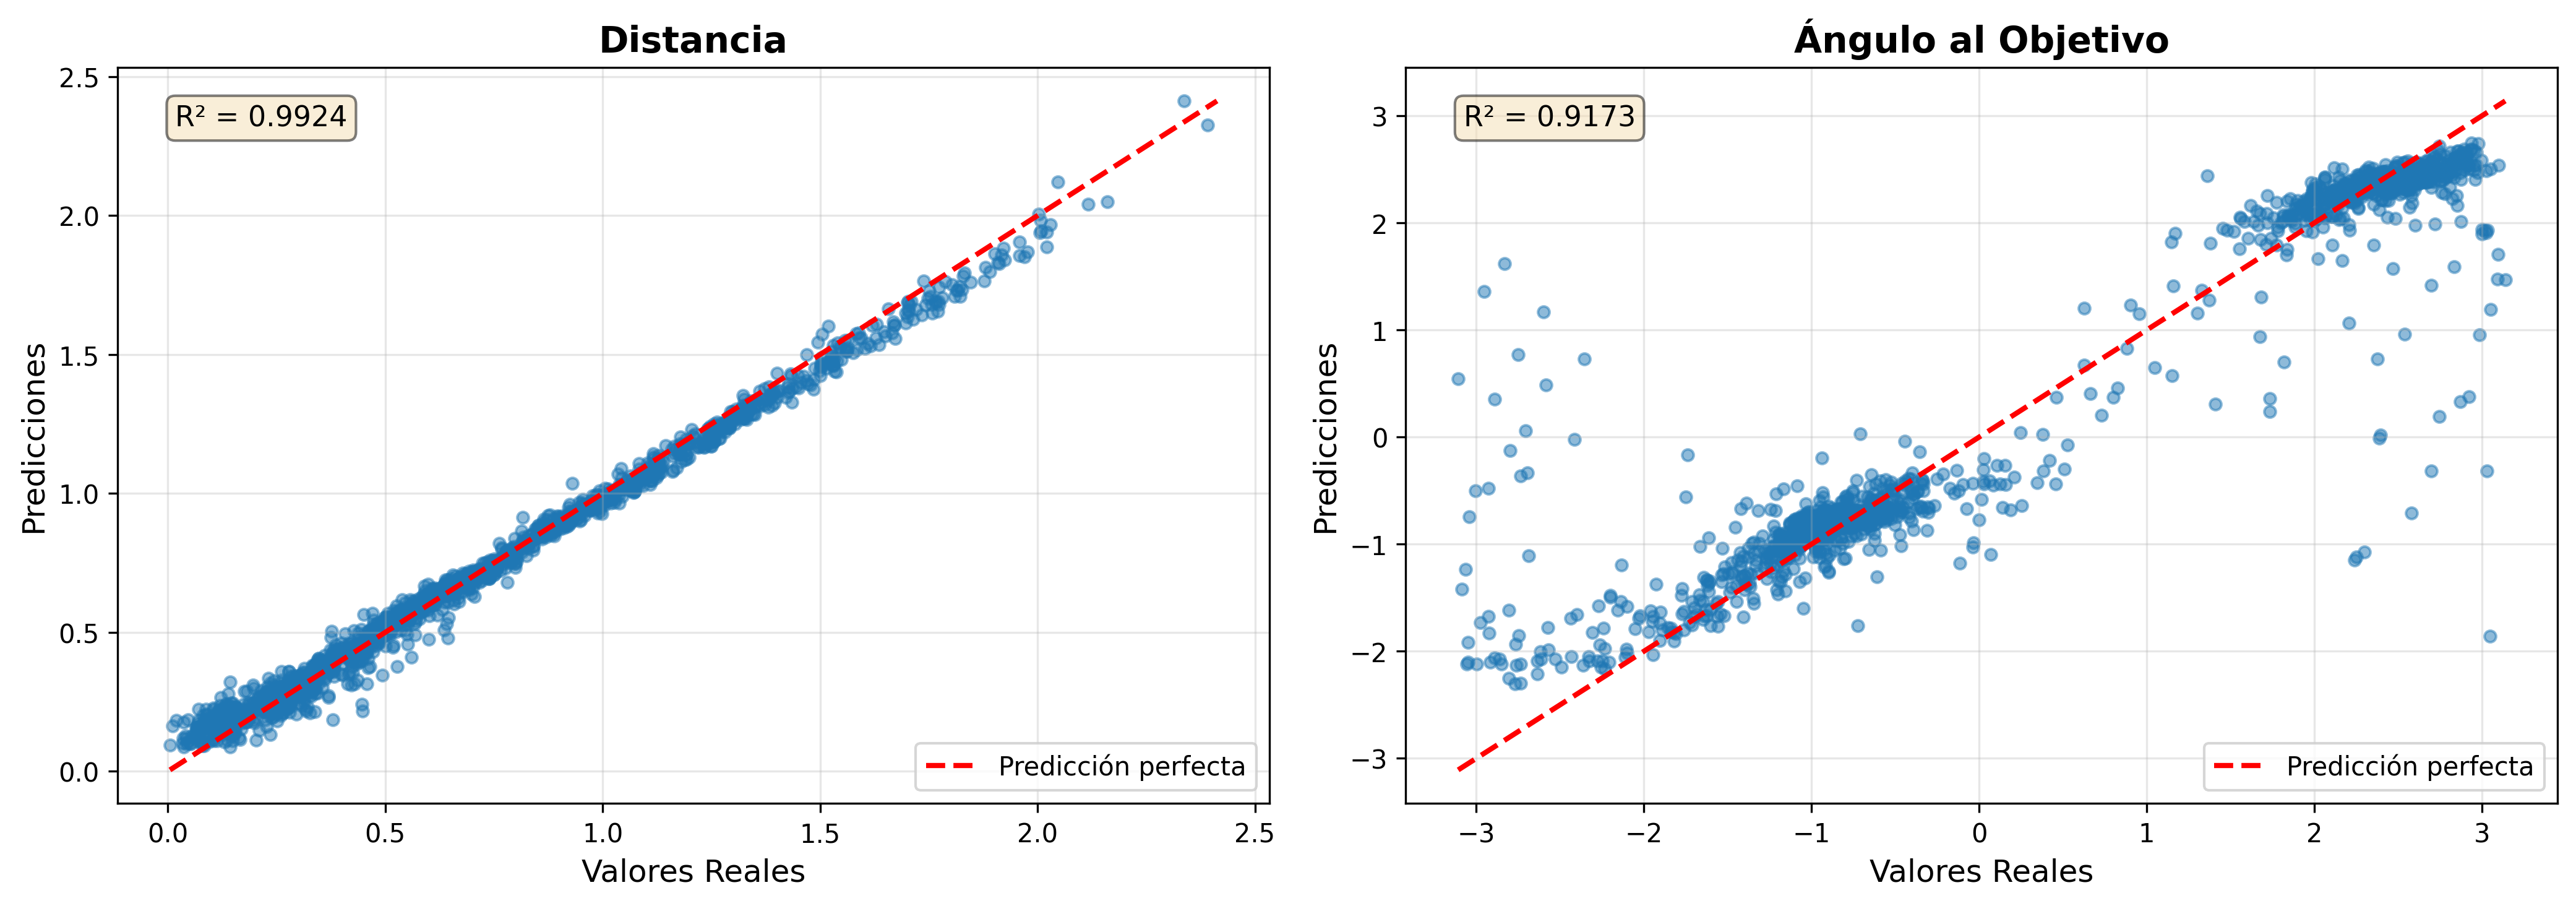
\includegraphics[width=\textwidth]{imaxes/BrazoRobot/WM_Brazo_Predicciones.png}
  \caption{Predicciones del modelo de mundo para el brazo robot.}
  \label{fig:brazorobot_WM_predictions}
\end{figure}

Tras entrenar este modelo de mundo, se integró con el modelo de utilidad creado originalmente para el robot Go2, añadiendo las modificaciones a en las entradas y salidas explicadas previamente 
para hacerlos compatibles. Al no contar con una interfaz de simulación para visualizar cómo se comporta el brazo robótico, se realizó mostrando en la consola como avanzaba la posición de este 
en cada iteración. En la figura \ref{fig:brazorobot_iteracion} se muestra un ejemplo de una iteración de este sistema. En ella se observa como, para el estado actual, el sistema comprueba todas 
las acciones disponibles, prediciendo el estado resultante con el modelo de mundo y evaluandolo con el modelo de utilidad original. Finalmente, selecciona la acción con mayor valor de 
utilidad, la cual es la que acerca más el brazo al objetivo.

\begin{figure}[hp!]
  \centering
  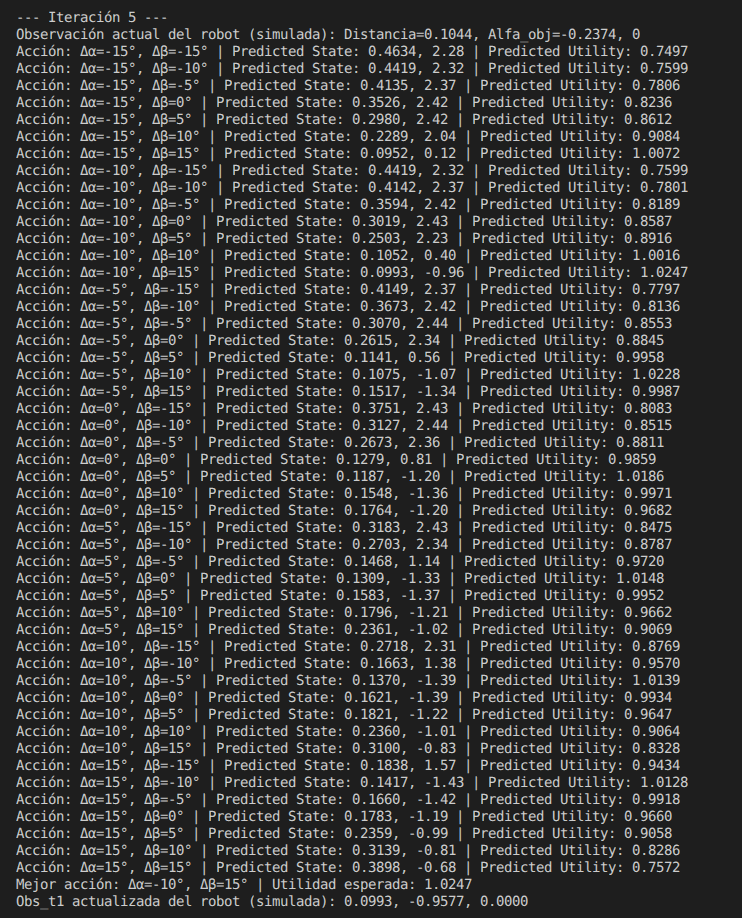
\includegraphics[width=\textwidth]{imaxes/BrazoRobot/Brazo_Robot_it_5.png}
  \caption{Ejemplo de una iteración en la simulación del brazo robot.}
  \label{fig:brazorobot_iteracion}
\end{figure}
